%*******************************************************************
%   Project Name: BracU Thesis Template (CSE400, Fall 2024 onwards)
%   Prepared by: Ayesha Abed Library, Brac University
%
%   Used here for the B.Sc. final year PROJECT report:
%   "AI-Powered Legal Document Analysis System (CUAD)"
%   Compile:  tectonic main.tex      (or on Overleaf: pdfLaTeX + Biber)
%*******************************************************************
% Project Structure:
% appendix: Contains "appendix.tex" files.
% bibliography: Contains "references.bib" file.
% chapters: Contains "chapter.tex" files.
% core: titlepage, declaration, approval, ethics_statement, abstract,
%       acknowledgement, nomenclature
% images: Contains all images files.
%*******************************************************************

\documentclass[Times,12pt,oneside,openany,print,index]{report}
\usepackage[a4paper,width=150mm,top=25mm,bottom=25mm]{geometry}
\usepackage[english]{babel}
\usepackage[utf8]{inputenc}
\usepackage{csquotes} % Provides advanced facilities for in-line and display quotations
\usepackage{amsmath} % TO use mathematical equations
\usepackage{amssymb}
\pagestyle{plain} % Just a plain page number.

\usepackage{graphicx} % to use the graphicx package
\graphicspath{{images/}} % Path to Image files
\usepackage{caption} % To use caption with figure and images
\usepackage{array} % column alignment in tables

\usepackage[nottoc]{tocbibind} % add ToC/bibliography etc. to the Table of Contents

\usepackage[normalem]{ulem} % underlining

% ---- additional packages needed by the project content ----
\usepackage{booktabs}     % \toprule, \midrule, \bottomrule, \addlinespace
\usepackage{adjustbox}    % shrink wide tables to the text width
\setlength{\emergencystretch}{3em} % fewer overfull lines
\usepackage{longtable}    % multi-page tables (risk taxonomy)
\usepackage{multirow}
\usepackage{enumitem}     % compact lists
\usepackage{setspace}     % \singlespacing inside table notes
\usepackage{xcolor}
\usepackage{tikz}         % pipeline diagrams
\usetikzlibrary{arrows.meta, positioning, shapes.geometric,
                decorations.pathreplacing, calc, fit, backgrounds, patterns}
\definecolor{riskhigh}{HTML}{D94F5C}
\definecolor{riskmed}{HTML}{E8A13A}
\definecolor{risklow}{HTML}{4CAF82}
\setcounter{tocdepth}{2}

\usepackage{hyperref} % Provides LaTeX the ability to create hyperlinks within the document.
\hypersetup{
    colorlinks=true,
    linkcolor=black,
    filecolor=magenta,
    urlcolor=black,
    citecolor=black,
}
\urlstyle{same}

\setlength{\parindent}{0em} % To control Indentation of paragraphs
\setlength{\parskip}{6pt} % space between paragraphs (none indent)

\usepackage[backend=bibtex,style=ieee,sorting=none]{biblatex} % IEEE citation style
\addbibresource{bibliography/references.bib} % Imports bibliography file

\let\cleardoublepage=\clearpage % removes unwanted doublepages

\begin{document}

\thispagestyle{empty} % removes page number from title page
\begin{titlepage}
\renewcommand*{\thepage}{Title} % Change page number in PDF

    \begin{center}
        \vspace*{3cm} % For creating Vertical Blank Space

        {\fontsize{16pt}{22pt}\selectfont{AI-Powered Legal Document Analysis System:\\
        Clause Detection, Category-Level Risk Prioritization\\
        and Plain-Language Explanation on CUAD}
        } % "fontsize{font size}{line space}\selectfont{}" command to override font size and line space for the Title

        \vspace{1.5cm}

        \text{by}

        \vspace{0.5cm}

        	Jerin Aktar\\
	        22101279\\
	        Afnan Mazumdar\\
	        24141229\\
	        Shoyeb Hasan Sayem\\
	        22101386

        \vspace{1.5cm}

        	A project submitted to the Department of Computer Science and Engineering\\
            in partial fulfillment of the requirements for the degree of\\
            B.Sc. in Computer Science and Engineering


        \vspace{2.5cm}

    		Department of Computer Science and Engineering\\
            Brac University\\
            July 2026

        \vspace{3cm}

    		\copyright\ 2026. Brac University\\
            All rights reserved.

    \end{center}

\end{titlepage}
 % Add title page
\cleardoublepage

\pagenumbering{roman} % Roman numbers to be use all pages before Chapter 1

\phantomsection
\addcontentsline{toc}{chapter}{Declaration}
% Following command is used to created grouped signature line for Four Authors
\newcommand*\wildcard[2][6cm]{\vspace{2cm}\parbox{#1}{\hrulefill\par#2}}

% A "parbox{}{}" is a box whose contents are created in paragraph mode.
% "hrulefill{} to chance thickness of underline"

\section*{Declaration}

It is hereby declared that

\begin{enumerate} % begin{enumerate} function to create numbered list
  \item The project submitted is our own original work while completing degree at Brac University.
  \item The project does not contain material previously published or written by a third party, except where this is appropriately cited through full and accurate referencing.
  \item The project does not contain material which has been accepted, or submitted, for any other degree or diploma at a university or other institution.
  \item We have acknowledged all main sources of help.
\end{enumerate}

\vspace{1cm}
\textbf{Student's Full Name \& Signature:} % Testbf{} for Bold

\begingroup

    \begin{center} % one signature block per line, stacked vertically
        \wildcard{\centerline{Jerin Aktar} ~\\ \centerline{22101279}} % "centerline{}" to center line
        \par
        \wildcard{\centerline{Afnan Mazumder} ~\\ \centerline{24141229}}
        \par
        \wildcard{\centerline{Shoyeb Hasan Sayem} ~\\ \centerline{22101386}}
    \end{center}

\endgroup


\pagebreak


\phantomsection
\addcontentsline{toc}{chapter}{Approval}
\section*{Approval}

The project titled ``AI-Powered Legal Document Analysis System: Clause Detection, Category-Level Risk Prioritization and Plain-Language Explanation on CUAD'' submitted by
\begin{enumerate}
  \item Jerin Aktar (22101279)
  \item Afnan Mazumder (24141229)
  \item Shoyeb Hasan Sayem (22101386)
\end{enumerate}

of Summer, 2026 has been accepted as satisfactory in partial fulfillment of the requirement for the degree of B.Sc. in Computer Science and Engineering in July 2026.

\vspace{0.5cm}
\textbf{Examining Committee:}

\vspace{1cm}

Supervisor:\\
(Member)
\begin{center}
    \hspace{7cm} \wildcard{\centerline{Utsha Kumar Roy} ~\\ \centerline{Designation}~\\ \centerline{Department of Computer Science and Engineering}~\\ \centerline{Brac University} } \hspace{1cm}
\end{center}

Head of Department:\\
(Chair)
\begin{center}
    \hspace{7cm} \wildcard{\centerline{Sadia Hamid Kazi, PhD} ~\\ \centerline{Chairperson and Associate Professor}~\\ \centerline{Department of Computer Science and Engineering }~\\ \centerline{Brac University} } \hspace{1cm}
\end{center}

\pagebreak


\phantomsection
\addcontentsline{toc}{chapter}{Ethics Statement}
\section*{Ethics Statement}
This project uses the Contract Understanding Atticus Dataset (CUAD), a publicly released research dataset of 510 commercial contracts taken from public filings and annotated by legal experts under The Atticus Project. We did not collect or process any private, confidential, or personally sensitive documents, and no human subjects were involved. All experiments ran on our own hardware. The third-party models we fine-tuned (DistilBERT, FLAN-T5) and all supporting libraries are used under their open-source licenses, and every outside source is cited.

The system is a research prototype meant to assist contract review. It is not legal advice, and that is stated in the application itself. The ethical risks of relying on its output --- false reassurance from missed clauses, over-reliance by non-lawyers, jurisdiction mismatch, the perspective from which risk is scored, the unreviewed authorship of the risk levels, and privacy in a real deployment --- are discussed in detail in Section~\ref{sec:ethics}.
\pagebreak


\phantomsection
\addcontentsline{toc}{chapter}{Abstract}
\section*{Abstract}
This project builds and tests a system of three models for reviewing contracts automatically, using CUAD (510 contracts, 41 clause categories) and a held-out test set made of 20\% of the contracts. The system finds which clause types a contract contains, extracts the clause text, gives each clause type a High, Medium or Low risk level with a plain-English line, and runs as a working app. In our first setup, a DistilBERT model that reads the contract in windows lost to a simple TF--IDF model that reads the whole document (micro-F1 0.692 against 0.775), and the gap survived changes to the training data, seed, pooling rule and threshold. We then found that the model read only about half of each window. Once it reads the whole window and both models are tuned on the same validation split, the transformer ties the tuned baseline (0.797 against 0.785), an ensemble of the two beats it (0.809, with a 95\% interval for the lead of $[+0.011, +0.037]$), and a recall-first setting finds 90.3\% of High-risk clauses, against 63.1\% for the first setup's best ensemble. Extracting the clause text reaches a token-F1 of 0.764 when the model is given the right window. The fine-tuned summarizer outputs one of 41 sentences we wrote ourselves, word for word, for every input, and scores 0.116 against clause-specific references. A calibration map fitted on the held-out contracts lowers the confidence score's calibration error from 0.206 to 0.016. Over the whole system only 22.1\% of real clauses get through all three steps: the presence model now finds the right window 82.6\% of the time, but the span model then succeeds in only 28.0\% of those cases.

\vspace{1cm}
\textbf{Keywords:} legal NLP; CUAD; clause extraction; category-level risk prioritization; contract summarization; held-out evaluation
\pagebreak


\phantomsection
\addcontentsline{toc}{chapter}{Acknowledgment}
\section*{Acknowledgement}
First of all, all praise to the Almighty for allowing us to complete this project without any major interruption. We are grateful to our supervisor, Utsho Kumar Roy, for his guidance and patience through every phase of this work, and especially for insisting on a strict held-out evaluation: that one requirement shaped how honestly this report presents its results. Finally, we thank our families for their constant support and encouragement. Without them, this work would not have been possible.
\pagebreak


\renewcommand{\contentsname}{Table of Contents} % Rename TOC name from Contents to Table of Contents
\cleardoublepage
\phantomsection
\addcontentsline{toc}{chapter}{Table of Contents} % Add Table of Contents in TOC
\tableofcontents % To  generation of the Table of Contents

\listoffigures % To  generation of the List of Figure
\listoftables % To  generation of the Tables of Figure

\phantomsection
\addcontentsline{toc}{chapter}{Nomenclature}
\chapter*{Nomenclature}
The list below gives the abbreviations used in this report.

\vspace{0.5cm}
\begin{tabular}{p{3cm} p{11cm}}
BERT & Bidirectional Encoder Representations from Transformers\\
CI & Confidence Interval\\
CPU / GPU & Central Processing Unit / Graphics Processing Unit\\
CUAD & Contract Understanding Atticus Dataset\\
ECE & Expected Calibration Error\\
EM & Exact Match\\
FN / FP & False Negative / False Positive\\
IP & Intellectual Property\\
LLM & Large Language Model\\
LR & Logistic Regression\\
MIL & Multiple-Instance Learning\\
MPS & Metal Performance Shaders (Apple GPU backend)\\
NLP & Natural Language Processing\\
QA & Question Answering\\
ROUGE & Recall-Oriented Understudy for Gisting Evaluation\\
RQ & Research Question\\
SD & Standard Deviation\\
SEC & US Securities and Exchange Commission\\
SQuAD & Stanford Question Answering Dataset\\
TF--IDF & Term Frequency--Inverse Document Frequency\\
TN / TP & True Negative / True Positive\\
\end{tabular}

\clearpage
\textbf{Glossary of terms}
\begin{description}[itemsep=4pt]
  \item[AND-ensemble] A rule that reports a clause category only when both the TF--IDF model and the DistilBERT model say it is present.
  \item[Bootstrap] A way to measure uncertainty: the test contracts are drawn again at random, with repeats, many times, and the score is recomputed each time.
  \item[Calibration] Whether a model's score can be read as a real chance. A well-calibrated score of 0.8 is right about 80\% of the time.
  \item[Clause category] One of the 41 types of contract clause labeled in CUAD (for example \emph{Governing Law}, \emph{Non-Compete}, \emph{Cap on Liability}).
  \item[Contract-level split] A train/test split that puts each whole contract on one side, so no clause from a training contract can appear in the test set.
  \item[Max-pooling (over windows)] Scoring every window of a document and using the highest window score as the score for the whole document.
  \item[Micro-F1] One F1 score computed over all (contract, category) decisions together, so every decision counts the same.
  \item[Micro-F2] The same, but treating recall as twice as important as precision, so a missed clause costs more than a false alarm.
  \item[Presence classification] Deciding, for each clause category, whether a contract contains at least one clause of that category.
  \item[Recall-first setting] A setup whose rule and thresholds were chosen on the validation split to maximize micro-F2; Clausify uses one by default.
  \item[Retrieval ceiling] The most a ``search first'' design can ever find: a clause in a window that the search never picks can never be found.
  \item[Span extraction] Finding the exact text of a clause inside the contract, treated as a question-answering task.
  \item[Token-F1] How much the extracted text overlaps the real clause, word by word (1.0 means a perfect match).
  \item[Validation split] The 81 training contracts held out in the re-run to choose settings such as thresholds, so that the test contracts play no part in any choice.
  \item[Weaker party] The person or company signing the contract with less bargaining power; the risk table is written from their side.
\end{description}

\cleardoublepage

\pagenumbering{arabic} % To use page number 1,2,3 ..

\chapter{Introduction}
\section{Background}
Contracts are part of almost everything people and businesses do, but reading them takes a lot of time. A typical contract in our dataset is about 33{,}000 characters long (roughly 5{,}000 words), and the longest is more than 338{,}000 characters. Somewhere in all that text are the parts that really matter: who owns new intellectual property, whether there is a limit on how much you can owe, whether the contract renews on its own, and whether you are stopped from working with competitors after it ends. Having a lawyer read a contract takes hours and costs money that many people and small businesses cannot afford. So people often sign contracts they do not fully understand and take on risks they never noticed.

The Contract Understanding Atticus Dataset (CUAD) \cite{hendrycks2021cuad} was created to help automate this kind of review. It has 510 real business contracts in which legal experts marked every clause that belongs to one of 41 important categories. This marking work is said to be worth about two million US dollars of lawyers' time. However, CUAD only treats the problem as finding text: given a category, find the clause. Once it finds a clause such as ``Uncapped Liability'', it stops. It does not warn the reader what the clause means for them, it does not explain it in simple words, and it does not check how clauses affect each other.

\subsection{System at a Glance}
Chapter~4 explains the system in detail. Figure~\ref{fig:overview} shows the whole system in one picture. The system answers three questions about a contract, in order: \emph{what is in it}, \emph{where is it}, and \emph{what does it mean}. CUAD was built to test only the first two. The third step, shaded in the figure, is what this project adds.

\begin{figure}[ht]
\centering
\begin{adjustbox}{max width=\textwidth}
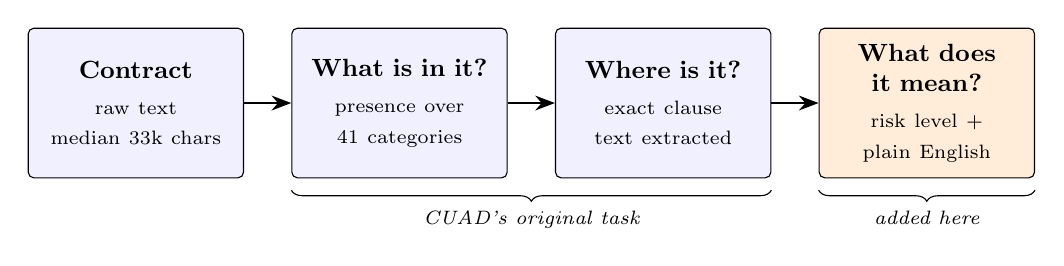
\begin{tikzpicture}[
  node distance=6mm,
  box/.style={draw, rounded corners=2pt, minimum height=19mm, text width=25mm,
              align=center, font=\small, fill=blue!6},
  new/.style={box, fill=orange!15},
  arr/.style={-{Stealth[length=2.5mm]}, thick}
]
\node[box] (a) {\textbf{Contract}\\[2pt]{\scriptsize raw text}\\{\scriptsize median 33k chars}};
\node[box, right=of a] (b) {\textbf{What is in it?}\\[2pt]{\scriptsize presence over}\\{\scriptsize 41 categories}};
\node[box, right=of b] (c) {\textbf{Where is it?}\\[2pt]{\scriptsize exact clause}\\{\scriptsize text extracted}};
\node[new, right=of c] (d) {\textbf{What does it mean?}\\[2pt]{\scriptsize risk level +}\\{\scriptsize plain English}};
\draw[arr] (a) -- (b);
\draw[arr] (b) -- (c);
\draw[arr] (c) -- (d);

\draw[decorate, decoration={brace, mirror, amplitude=4pt}]
  ($(b.south west)+(0,-1.5mm)$) -- ($(c.south east)+(0,-1.5mm)$)
  node[midway, below=4pt, font=\scriptsize\itshape] {CUAD's original task};
\draw[decorate, decoration={brace, mirror, amplitude=4pt}]
  ($(d.south west)+(0,-1.5mm)$) -- ($(d.south east)+(0,-1.5mm)$)
  node[midway, below=4pt, font=\scriptsize\itshape] {added here};
\end{tikzpicture}
\end{adjustbox}
\caption{Three questions the system answers}
\label{fig:overview}
\end{figure}

\section{Rationale of the Study or Motivation}
Our project tries to close the gap between finding a clause and understanding it. On top of finding clauses, we add two things. First, a simple risk table that gives every clause \emph{category} a High, Medium or Low level, judged from the side of the weaker party. Second, a text model that is meant to turn each clause into one plain-English sentence. We built the clause-finding models and the risk table into \emph{Clausify}, a prototype web app: a user pastes or uploads a contract and gets back a list of clauses sorted by risk. Both added parts worked less well than we hoped. The risk table has not been checked by a lawyer (Section~\ref{sec:taxvalid}), and the text model learned to repeat a fixed sentence for each category instead of describing the actual clause (Section~\ref{sec:summ}). Chapters~5 and~6 report these results honestly.

So the reason for this study is practical as well as academic. Earlier work on CUAD answers the question ``where is the clause?'' for a lawyer who already knows what to look for. The people who need help most (individuals, freelancers and small businesses who sign contracts without a lawyer) also need to know which clauses matter most to them and what each one means in everyday language. A system that gives those answers, and is honest about how often it is wrong, could make contract review possible for people who cannot pay for it today. Just as important, we wanted to measure how well such a system really works instead of assuming it. A contract-review tool that looks confident but quietly misses clauses is worse than having no tool at all.

\section{Problem Statement}
In short, the project works on four connected problems:
\begin{enumerate}[itemsep=2pt]
  \item \textbf{Finding which clauses are present.} For each of the 41 CUAD categories, decide whether a contract has at least one clause of that type. The main difficulty is length: a typical contract is about 16$\times$ longer than the amount of text a standard transformer model can read at once.
  \item \textbf{Finding the exact clause text.} For each category that is present, find the exact words of the clause in the contract. We treat this as a question-answering task, in the same style as SQuAD \cite{rajpurkar2016squad}.
  \item \textbf{Explaining in plain language.} Rewrite each clause as one sentence that a non-lawyer can understand.
  \item \textbf{Showing the risk.} Give every clause found a risk level and a one-line reason, so the result reads like a ranked list of warnings instead of a list of quotes. We did not test whether this actually helps users (Section~\ref{sec:threats}).
\end{enumerate}

\subsection{Research Questions}
\label{sec:rqs}
Our objectives turn into five research questions, which the rest of this report answers. We give the answers here so readers can check each claim against the evidence instead of searching for it.

\begin{description}[itemsep=4pt, leftmargin=1.6cm]
  \item[RQ1] \emph{Can a transformer that reads a contract in small windows beat a simple word-based model that reads the whole contract, at finding which clauses are present?}\\
  \textbf{No.} The simple model wins by $+0.082$ micro-F1. The gap stays even when the transformer is trained on all its training data (Section~\ref{sec:budget}) and with three different random seeds (Section~\ref{sec:seeds}). Answered in Chapter~5.
  \item[RQ2] \emph{How well can the system find the exact clause text in long contracts?}\\
  Token-F1 is 0.764 (95\% CI $[0.743, 0.782]$) \emph{when the model is given a window that contains the clause}, but only 0.383 when the window is chosen by the first model (Sections~\ref{sec:span} and~\ref{sec:e2e}).
  \item[RQ3] \emph{Does the summarizer really describe each specific clause in plain English?}\\
  \textbf{No.} For every input it copies one of 41 sentences we wrote in advance. Against clause-specific reference sentences, it scores no better than just printing that fixed sentence without any model (Section~\ref{sec:summ}).
  \item[RQ4] \emph{How do errors add up across the whole system?}\\
  They multiply, and it is worse than the separate scores suggest: only 22.0\% of real clauses get through all three steps, compared with the $\approx$65\% that the separate scores would predict (Section~\ref{sec:e2e}).
  \item[RQ5] \emph{Do the system's mistakes avoid the clauses that would hurt a signer most?}\\
  \textbf{No, the opposite.} The setup we report as our main result misses 36.9\% of High-risk clauses, while the model we call weaker misses only 15.9\% (Section~\ref{sec:riskeval}). The overall score and the harm to the user point in different directions.
\end{description}

Three of these five answers are negative. We report them as real results of the project, not as failures. Each one is something a reader would have got wrong by looking only at the separate model scores.

\section{Objective}
\begin{itemize}[itemsep=2pt]
  \item Build and fairly test a complete three-model CUAD system on an ordinary laptop, using an 80/20 split by contract so that every reported number comes from contracts the models have never seen.
  \item Check whether a transformer really beats a strong simple model at finding which clauses are present, instead of assuming it does.
  \item Measure how well the exact clause text is found, using token-level F1 and exact match on the test set.
  \item Test the summarizer against two different sets of reference sentences, because one automatic score turned out to measure the reference sentences rather than the task.
  \item Measure how many clauses survive the whole system from start to finish, not only the score of each step.
  \item Put the trained models into a working demo app that shows clauses sorted by risk.
\end{itemize}

\section{Methodology in Brief}
We tested every design before building on it, using one fixed 80/20 split of CUAD by contract (408 training contracts and 102 test contracts). After exploring the data (Section~\ref{sec:eda}), we first built a simple word-based model (TF--IDF with logistic regression) that reads the whole contract, \emph{before} training any transformer. We also measured the highest recall a ``search first'' design could ever reach (Section~\ref{sec:ceiling}). Based on that, we trained a DistilBERT model that scores the contract in small windows and takes the highest window score as the answer for the whole contract (multiple-instance learning). We combined it with the simple model using an AND rule, which reports a clause only when both models agree. A DistilBERT question-answering model finds the exact clause text, a fine-tuned FLAN-T5-small model writes a one-sentence plain-English explanation, and a hand-made table gives each of the 41 categories a High, Medium or Low risk level.

Every model was tested once on the 102 test contracts. We report each score together with confidence intervals from a bootstrap over contracts, and we checked how the results change with the amount of training data, the random seed, the way window scores are combined, the decision threshold and the train/test split. We also tested the full system from start to finish. Finally, we put the trained models into \emph{Clausify}, a Streamlit web app that gives a risk-sorted clause report for any contract. Chapter~4 describes the method in full.

\section{Scopes and Challenges}
\textbf{Scope.} The project covers English business contracts like those in CUAD: 510 contracts from US SEC filings, marked for 41 clause categories. Within that scope it handles four tasks (finding which clauses are present, finding their exact text, explaining them in plain language and showing their risk level) and delivers a working prototype app. The following are outside the scope on purpose: legal advice of any kind; contracts in other languages or countries (including Bangladeshi contracts, which inspired the work but were not tested); judging the risk of a clause's exact wording; finding conflicts between clauses; and a formal user study of the app. All models were sized so they can be trained and run on one ordinary laptop.

\textbf{Challenges.} Six challenges shaped the design:
\begin{enumerate}[itemsep=2pt]
  \item \textbf{Very long documents.} A typical contract is about 33{,}000 characters. That is roughly 16$\times$ the 512-token limit of a standard transformer (about 2{,}000 characters), and the longest contract is more than 338{,}000 characters, about 170$\times$.
  \item \textbf{Very uneven categories.} Some categories appear in 100\% of contracts and some in only 2.5\%; a few have only a handful of examples in the whole dataset.
  \item \textbf{A small, fixed dataset.} The 510 contracts are all there is, and expert marking is too costly to add more, so we had to be careful about over-fitting and about test data leaking into training.
  \item \textbf{Limited hardware.} Training ran on an Apple-Silicon laptop without a CUDA GPU. Our first-choice model (DeBERTa-v3) was unstable on the MPS backend, and GPU memory was not freed between training runs.
  \item \textbf{No plain-language answers to learn from.} CUAD has no plain-English versions of clauses, so we had to write our own reference sentences, and this limited what the summarizer could learn.
  \item \textbf{No agreed answer for risk either.} Contract risk depends on which side you are on, the situation and the country, and there is no expert-checked risk model for CUAD's 41 categories.
\end{enumerate}

\section{Report Organization}
The rest of this report is organized as follows. Chapter~2 reviews background and earlier work. Chapter~3 sets out the system's requirements, its effect on society, the environment, ethics and cost, and the project plan. Chapter~4 explains the method: how we designed the system, which other designs we considered, how the data was prepared, and how the models and the Clausify app were built. Chapter~5 analyses the results on the test set, including the statistics and the changes we made because of them. Chapter~6 sums up the findings, contributions and limits, and suggests future work. The appendices contain the full 41-category risk table, a checklist for repeating the work and the layout of the project files.



\chapter{Literature Review}
\section{Preliminaries}
This section explains the models and methods the project is built on.

\subsection{Transformer Encoders and Model Distillation}
The transformer \cite{vaswani2017attention} is a type of neural network that reads text with self-attention instead of word by word. BERT \cite{devlin2019bert} showed a simple recipe that this project relies on: first train a model on a very large amount of general text, then fine-tune it for a specific task on a much smaller amount of labelled data. The recipe suits us, because 510 contracts is a small dataset for deep learning.

Because all our work runs on one laptop, we use DistilBERT \cite{sanh2019distilbert}, a smaller, six-layer version of BERT that keeps about 97\% of BERT's language ability while being 40\% smaller and 60\% faster. The published CUAD results use much larger models, so we give up some accuracy in exchange for running everything on normal hardware. We point out this size difference whenever we discuss our results.

\subsection{Long-Document Strategies and Multiple-Instance Learning}
\label{sec:lit_long}
Contracts are much longer than a transformer can read at once. There are three usual ways to deal with this: (i) \emph{retrieval}, where a quick, cheap method picks the few parts of the text most likely to contain the answer and only those go to the transformer; (ii) \emph{sliding windows}, where the model reads every part of the text and the scores are combined into one answer for the whole document; and (iii) \emph{sparse-attention models} such as Longformer, which can read a longer piece of text at once.

The third option is often dismissed in one line as ``too expensive'', which is not enough of a reason. We did not run a Longformer experiment, so what follows is a design choice. The one part of it we could check cheaply on our own laptop was the cost, and Section~\ref{sec:lfbench} reports that check.

We had three reasons, and only the third is about cost. The first and most important is that Longformer would not solve the problem. It can read 4{,}096 tokens at once. At about four characters per token, our typical contract of 33{,}143 characters is about 8{,}300 tokens and the longest is about 85{,}000, so Longformer would still see only half of a typical contract and one-twentieth of the longest one. It makes the window eight times wider, which is still not wide enough for this data. We would still need windows and a way to combine their scores, which is the design we ended up using anyway, only with a much more expensive model underneath. This reason comes from arithmetic about the dataset and not from an experiment, but the arithmetic is clear: CUAD contracts are about ten times too long for a wider window to fix.

The second reason is availability. Our whole system uses small (distilled) models so that it can be trained and run on one laptop. We do not know of a small version of Longformer that is as reliable and well supported as DistilBERT, so using Longformer would have meant giving up the small models that make the rest of the project easy to repeat.

The third reason is cost in practice. We believed that fine-tuning a Longformer with 148.7M parameters at 4{,}096 tokens was not possible on one Apple-Silicon laptop. We were also worried about special attention code on a non-CUDA machine, after DeBERTa-v3 produced NaN (broken) values on the MPS backend (Section~\ref{sec:engineering}). When we later measured it (Section~\ref{sec:lfbench}), the memory part of this belief turned out to be wrong, since one training step does fit at batch size 1. The time part was right by a very large margin. We kept our original reasoning in the text and reported the correction next to the measurement, so the reader can see both. The app adds its own cost: \emph{Clausify} scores every window of an uploaded contract for all 41 categories while the user waits, so it is only usable if this takes seconds. That can be measured without any training, and Section~\ref{sec:lfbench} gives the speed and peak memory of Longformer-base at 4{,}096 tokens on our laptop, next to the DistilBERT setup we used.

On a CUDA computer with more memory, the third reason would be weaker and the second might disappear, but the first would still hold. The choice is backed by one measurement and some arithmetic. It does not prove that sparse attention cannot work on CUAD. A properly trained Longformer with windows would be a fair comparison to ask for, and we list it as future work.

Reading a document in windows and taking the highest window score is known as \emph{multiple-instance learning} (MIL). The document is treated as a bag of windows, and the bag counts as positive if any one window is positive, which is what taking the maximum score does. MIL has a well-known weakness, and our experiments confirmed it: it produces too many false alarms. A document has dozens of windows, so the chance that some window fires by mistake grows with the length of the document, and precision drops.
\subsection{Text-to-Text Models for Summarization}
T5 \cite{raffel2020t5} treats every language task as ``text in, text out'', which suits clause simplification: legal text goes in and a simple sentence comes out. FLAN-T5 \cite{chung2022flan} is a version of T5 trained on many tasks with instructions, so it already gives useful answers to a simple prompt such as ``summarize in plain English:'' without extra training. We score summaries with ROUGE-L \cite{lin2004rouge}, which measures how many words the output shares, in the same order, with a reference sentence. Chapter~5 shows why, when there are only a few reference sentences, this score has to be checked by reading the outputs.

\section{Review of Existing Research}
This section reviews earlier work on legal language processing, legal risk, plain-language legal writing, and the accuracy of machine-written summaries.

\subsection{Legal NLP and the CUAD Benchmark}
People have long wanted to use language technology on legal text, and progress was slow for a simple reason: labelling legal text needs lawyers, and lawyers are expensive. CUAD \cite{hendrycks2021cuad}, released by The Atticus Project \cite{atticus2021} at the NeurIPS 2021 Datasets and Benchmarks track, changed this. It provides 510 real business contracts from public SEC filings, in which experienced lawyers marked every piece of text that belongs to one of 41 important clause categories, such as governing law, non-compete, limits on liability and IP assignment. The data uses the SQuAD format \cite{rajpurkar2016squad}: each (contract, category) pair is asked as a question about the contract text, and the marked clauses are the answers, with their exact character positions.

The original CUAD paper treats the task as question answering and finds that bigger models do much better. Its best results come from the extra-large DeBERTa models, and even those scores are modest, which shows how hard it is to find legal clauses. Two features of CUAD affect any model built on it. Categories are very uneven: some appear in almost every contract, while others appear only about a dozen times in the whole dataset. Contracts are also long, far longer than a transformer can read at once, so every practical system first has to work out how a model that reads 512 tokens at a time can read a 50{,}000-character contract.
\subsection{Legal Risk Assessment and Decision Support}
\label{sec:lit_risk}
The risk part of this project has the least earlier work behind it, which is a weakness of our work. Since we tell a non-lawyer which clauses to worry about, the obvious question is what this advice is based on. We did not use an existing framework. We wrote the risk table ourselves (Section~\ref{sec:riskcriteria}), which is why we call it a prototype.

Earlier work does explain why this is hard. Legal language benchmarks usually treat ``risk'' indirectly, by sorting text into legally meaningful categories without judging how serious something is. LexGLUE \cite{chalkidis2022lexglue} collects tasks such as predicting court decisions and classifying laws, and LEGAL-BERT \cite{chalkidis2020legalbert} shows that models pre-trained on legal text do better on them. None of these tasks asks how dangerous a clause is for a particular person signing it. CUAD itself \cite{hendrycks2021cuad} describes its categories as the clauses lawyers look for when checking a deal, which marks them as important without saying how important.

How serious a clause is remains an open question, and it is hard to learn from data alone, for three reasons. Risk depends on which side you are on: the same unlimited indemnity is dangerous for the party giving it and useful for the party receiving it, so a risk label only makes sense once you pick a side, a problem Section~\ref{sec:weaker} handles only by making an assumption. Risk depends on the situation, since a \$50{,}000 limit on liability means little to a large company but can ruin a one-person business. And risk depends on the country, since a non-compete that is binding in one country may be invalid in another. Our table gives one fixed level per category, so it ignores all three on purpose.

This affects how our work should be read. Our risk table should be compared with expert opinion, because we know of no published model that covers CUAD's 41 categories, and that expert check has not been done yet (Section~\ref{sec:taxvalid}). Work on explainable legal AI argues that tools in this area should show their reasoning instead of just giving a score. Our table does this: every level comes with a written reason that can be questioned line by line (Appendix~\ref{app:taxonomy}). That openness makes the table easy to check, though it does not make the table correct.
\subsection{Plain-Language Legal Communication}
\label{sec:lit_plain}
Chapter~5 finds that our summarizer does not really summarize, and the closest earlier work is about simplifying text. The two goals differ. Summarizing makes text shorter, while simplifying says the same thing in easier words. For a contract clause, shorter is often the wrong goal, because the conditions and exceptions a summary would drop are often what decides what the clause does.

The closest earlier work is Manor and Li \cite{manor2019plain}, who collected plain-English summaries of contract sections and found that models trained on them tend to give general, repeated answers, an early version of the problem our template test measures. Measuring how easy a text is to read is a much older field \cite{flesch1948}, and it offers a check our evaluation lacks: that the output is easier to read, and not only shorter. We do not report any readability score. Looking back, that is a gap, since this part of the project exists to make clauses easier to understand.

Our results agree with the main lesson of this work: scores based on reference sentences measure the reference sentences. With only 41 different target sentences, ROUGE-L rewards the model for recognising the category. Section~\ref{sec:summ} measures this directly by changing the reference sentences while keeping everything else the same.
\subsection{Faithfulness and Hallucination in Generated Summaries}
\label{sec:lit_faith}
When a system shows machine-written sentences next to a user's own contract, whether those sentences are true is a safety issue. Research on summarization has shown that fluent machine-written summaries often say things that are not in the source. Maynez et al.\ \cite{maynez2020faithfulness} find that many generated summaries contain content the input does not support, and that ROUGE agrees poorly with human judgements of accuracy. Kry\'{s}ci\'{n}ski et al.\ \cite{kryscinski2020factcc} suggest checking factual accuracy as a separate task. Scores such as BERTScore \cite{zhang2020bertscore} measure meaning better than simple word overlap, but they do not check facts either.

Our system has an unusual version of this problem. A model that only outputs fixed template sentences cannot invent details in the usual way, because it can only produce one of 41 sentences written by people, and each one correctly describes its category. It fails in the opposite way. It says nothing about the specific clause, and when it picks the wrong template (30\% of the time, Section~\ref{sec:summ}) the output is fluent and confident but describes a completely different kind of clause. For a legal assistant this may be worse than an invented detail, because the output gives no sign of the error. The sentence is well written and true of its own category, and only a comparison with the clause shows that it does not describe it.

Our evaluation is therefore missing the checks this research recommends. We report ROUGE-L against two sets of reference sentences and we read outputs by hand. We do not report BERTScore, an automatic fact check, or a human judgement of whether the legal meaning is kept, and for a part that non-lawyers will see, the human judgement matters most. Section~\ref{sec:futurework} lists it as future work.

\section{Summary of Key Findings}
\label{sec:litgap}
Earlier CUAD work stops once the clause is found. A person signing a contract probably needs more: which clauses matter, how much, and what they mean in plain language. This project tries to add that layer, with a prototype risk table for each category, plain-English template sentences and a demo app. It also re-tests, on a strict test set, the common belief that a transformer must beat simple word-based methods at deciding which clauses a contract contains. Of the three added parts, the results support only the demo app as working. No expert has checked the risk table, and the plain-English part outputs category templates instead of summaries, so neither is solved. The added layer mostly gives a measurement of how far it is from working.

Table~\ref{tab:related} compares this work with the earlier work above. The first difference is scope. Earlier work stops at finding the clause text, while our output is a risk-sorted, plain-English report, which is the part a non-lawyer can act on. The second is in the ``Long inputs'' column. Every system on CUAD must choose how to handle long documents, and usually the choice is just stated. We measured ours before any training: the 64.0\% retrieval limit in Section~\ref{sec:ceiling} ruled out retrieval and led us to multiple-instance learning. The Model column also shows a cost. Our small models (67M parameters) are about ten times smaller than the DeBERTa-xlarge model behind CUAD's best published result, so our extraction scores cannot be compared directly with theirs, and we do not claim they can.

\begin{table}[!ht]
\centering
\caption{Related work}
\label{tab:related}
\footnotesize
\setlength{\tabcolsep}{3.5pt}
\renewcommand{\arraystretch}{1.25}
\hyphenpenalty=10000
\newcolumntype{L}[1]{>{\raggedright\arraybackslash}p{#1}}
\newcommand{\ds}[1]{\newline{\scriptsize\color{gray!70!black}#1}}
\begin{adjustbox}{max width=\textwidth}
\begin{tabular}{@{}L{25mm} L{23mm} L{21mm} L{25mm} L{17mm} L{16mm} L{23mm}@{}}
\toprule
\textbf{Work \textnormal{(data)}} & \textbf{Task} & \textbf{Model} & \textbf{Long inputs} & \textbf{Risk} & \textbf{Plain English} & \textbf{Evaluation}\\
\midrule
Hendrycks et al.\ \cite{hendrycks2021cuad}\ds{CUAD, 510 contracts}
 & Span extraction & DeBERTa-xlarge & Full-document QA with a large model & No & No & Held-out; precision at 80\% recall\\
\addlinespace
Chalkidis et al.\ \cite{chalkidis2020legalbert}\ds{several legal corpora}
 & Domain pre-training and classification & LEGAL-BERT & Truncation to 512 tokens & No & No & Per-task held-out\\
\addlinespace
Chalkidis et al.\ \cite{chalkidis2022lexglue}\ds{LexGLUE, 7 tasks}
 & Legal language understanding & BERT and RoBERTa models & Depends on the task & Indirect (task labels) & No & Multi-task benchmark\\
\addlinespace
Manor and Li \cite{manor2019plain}\ds{TL;DR-Legal style}
 & Plain-English summarization & Seq2seq & Section-level inputs & No & \textbf{Yes} & ROUGE and manual review\\
\addlinespace
Beltagy et al.\ \cite{beltagy2020longformer}\ds{long-document benchmarks}
 & New architecture & Longformer & Sparse attention, 4{,}096 tokens & No & No & Task benchmarks\\
\addlinespace
Retrieval--QA pipelines\ds{various}
 & Span extraction & Various & Retrieval then reader (ceiling usually assumed) & No & No & Various\\
\midrule
\rowcolor{blue!6}
\textbf{This project}\ds{CUAD, 510 contracts}
 & Presence, span, category risk and template text
 & DistilBERT and FLAN-T5 (small)
 & Sliding-window MIL; ceiling \emph{measured}, sparse attention \emph{benchmarked}
 & \textbf{Yes} (category level, prototype)
 & \textbf{Yes} (template based)
 & Contract-level held-out; cluster bootstrap; seed, budget and split controls; end-to-end\\
\bottomrule
\end{tabular}
\end{adjustbox}

\vspace{4pt}
{\footnotesize\singlespacing \emph{Note.} ``Long inputs'' is how each work handles documents longer than the encoder window; ``Evaluation'' is the level at which results are reported.\par}
\end{table}



\chapter{Requirements, Impacts and Constraints}
\section{Final Specifications and Requirements}
\subsection{Functional requirements}
\begin{enumerate}[label=\textbf{FR\arabic*}, itemsep=2pt, leftmargin=1.4cm]
  \item The system shall accept a contract as pasted text or as an uploaded \texttt{.txt} file.
  \item For each of the 41 CUAD clause categories, the system shall decide whether the contract contains a clause of that category and report a confidence score.
  \item For each category judged present, the system shall extract and display the clause text from the user's own contract.
  \item The system shall attach a High, Medium or Low risk level and a one-line plain-English reason to every detected clause.
  \item The system shall present detected clauses grouped by risk level (High first) and sorted by confidence within each group.
  \item The user shall be able to adjust the detection threshold, and the system shall expose the raw score of all 41 categories.
\end{enumerate}

\subsection{Non-functional requirements}
\begin{itemize}[itemsep=2pt]
  \item \textbf{Privacy.} All inference shall run locally; no contract text shall be transmitted to a third-party service or written to disk.
  \item \textbf{Hardware feasibility.} All models shall train and run on a single consumer laptop without a CUDA GPU.
  \item \textbf{Responsiveness.} Analysis of a typical contract shall complete within tens of seconds on CPU (measured: median 27.1\,s, worst case 32.4\,s; Table~\ref{tab:appbench}).
  \item \textbf{Validity of evaluation.} Every reported metric shall come from contracts never seen in training (contract-level split), and no hyperparameter shall be selected on the test set.
  \item \textbf{Reproducibility.} The split, the fitted baseline and all trained weights shall be saved, and a standalone notebook shall regenerate every reported number from them.
  \item \textbf{Transparency.} The application shall state that it is not legal advice, and every risk assignment shall carry a written justification (Appendix~\ref{app:taxonomy}).
\end{itemize}

\subsection{Data and resource requirements}
Table~\ref{tab:resources} lists the data, hardware and software the project depends on. All of it is either publicly available at no cost or was already owned by the team.

\begin{table}[ht]
\centering
\caption{Data, hardware and software requirements.}
\label{tab:resources}
\small
\begin{adjustbox}{max width=\textwidth}
\begin{tabular}{p{3.2cm} p{10.2cm}}
\toprule
\textbf{Resource} & \textbf{Specification}\\
\midrule
Dataset & CUAD v1 (The Atticus Project), 510 annotated contracts: \texttt{master\_clauses.csv} and \texttt{CUAD\_v1.json}, obtained from the Hugging Face hub\\
Hardware & Apple M4 laptop, 16\,GB unified memory, MPS (Metal) GPU backend; no CUDA GPU\\
Language and runtime & Python 3.13.5\\
Deep learning & PyTorch 2.8.0, Hugging Face \texttt{transformers} 5.12.1, \texttt{datasets} 5.0.0\\
Classical ML and data & scikit-learn 1.6.1, NumPy 2.1.3, pandas 2.2.3, \texttt{rouge\_score}\\
Pre-trained models & \texttt{distilbert-base-uncased} (presence and span), \texttt{google/flan-t5-small} (summarizer)\\
Application & Streamlit ($\geq$1.40) single-page web application\\
Development tools & Jupyter notebooks, Git and GitHub, \LaTeX\\
\bottomrule
\end{tabular}
\end{adjustbox}
\end{table}

\subsection{Design constraints}
The requirements above interact with four constraints that determined the final design. \textbf{Compute:} a single laptop rules out large backbones such as DeBERTa-v3-XL used in the original CUAD work, so distilled models were chosen. \textbf{Data:} 510 contracts cannot be extended, which makes transfer learning mandatory and the contract-level split essential. \textbf{Latency:} the application must score every window of a contract for all 41 categories, which motivated the 30-window cap in the deployed system. \textbf{Privacy:} the requirement for local inference excludes hosted language-model APIs entirely.

\section{Societal Impact}
\textbf{Access to legal understanding.} Contract review by a lawyer takes hours and costs money that individuals and small businesses often cannot afford, so many people sign agreements they have not fully understood. A tool that points a non-lawyer to the provisions most likely to hurt them --- uncapped liability, IP assignment, non-competes, automatic renewal --- can lower that barrier and help people ask the right questions before signing. The intended users include freelancers, start-ups and small businesses, groups for whom professional review is least affordable.

\textbf{Health and safety.} The system has no direct physical health or safety implications. Its indirect effect is financial and psychological: a contract signed without understanding can lead to disputes, losses and stress, which better-informed signing could reduce.

\textbf{Legal implications.} The system is not legal advice, and it says so. Its most important societal risk is \emph{false reassurance}: a missed clause produces no warning, and the absence of a warning can be read as ``nothing to worry about''. Our measurements show this risk is real --- only 21.7\% of gold clauses survive the complete pipeline (Section~\ref{sec:e2e}) --- so the tool must be positioned as an aid to reading a contract, never as a substitute for professional review.

\textbf{Cultural and regional aspects.} CUAD consists of US commercial contracts written in English. Risk levels that are reasonable under US law may not hold elsewhere, and drafting conventions differ between jurisdictions. Although the motivating context for the work is Bangladesh, no Bangladeshi contract was tested, so the benefits above cannot yet be claimed for that context.

\section{Environmental Impact}
The project was designed to be computationally light. All models are distilled or small (DistilBERT with 67M parameters and FLAN-T5-small), training of the three deployed models took roughly 1.5 hours on a laptop, and the deployed application runs on CPU with a peak memory footprint of about 1.5\,GB (Table~\ref{tab:appbench}).

Adding the control experiments --- the full-data presence run (140.7 minutes), two additional seeds, the evaluation passes and the Longformer benchmark --- the total compute for the project is in the order of ten laptop-hours. Assuming a sustained power draw of 20--30\,W for an Apple-Silicon laptop under load (an estimate, not a measurement), this corresponds to well under one kilowatt-hour of electricity, a negligible footprint compared with the multi-GPU training typically used for large legal language models.

Two design decisions keep the operating footprint small as well. Inference is local, so no data-centre resources are consumed per analysed contract, and the system avoids large generative models whose per-query energy cost is far higher. The trade-off is accuracy: Section~\ref{sec:lfbench} shows that larger architectures were rejected partly on cost, and Chapter~5 reports what the small models achieve.

\section{Ethical Issues}
\label{sec:ethics}
The front-matter Ethics Statement records how the data and models were obtained. This section examines the ethical issues that arise from the \emph{use} of the system, and the professional responsibilities they place on its designers.

The system is a research prototype meant to assist contract review. It is not legal advice, and the application states this in a notice shown above every analysis. For a tool of this kind the more serious ethical questions are not about the dataset but about what happens if someone relies on the output, so we set them out explicitly.

\textbf{False reassurance is the primary hazard.} A clause the system does not detect produces no warning, and an absent warning is easily read as ``there is nothing here to worry about''. Our measurements say that reading would be wrong: 22.0\% of gold clauses are missed at the presence stage, only 21.7\% survive the full pipeline (Section~\ref{sec:e2e}), and the configuration we report as our headline misses 37.5\% of the High-risk clauses specifically (Section~\ref{sec:riskeval}). A user who reviews a contract with this tool and sees three warnings has not established that there are only three problems. This asymmetry --- silent false negatives versus visible false positives --- is why we regard High-risk recall as the ethically relevant metric even though it is not the one the aggregate optimizes.

\textbf{Over-reliance by non-lawyers.} The interface is designed for people without legal training, which is exactly the audience least able to detect when it is wrong. Plain-English text presented with a confidence bar carries an authority the underlying model does not earn --- and Section~\ref{sec:threshold} shows the confidence bar is not even calibrated: scores above 0.9 correspond to roughly a 73\% chance of the clause being present. The plain-English reason on each clause card is a fixed sentence per category from the risk taxonomy, not a reading of the user's clause; the summarizer that was meant to provide clause-specific text also turned out to emit category templates (Section~\ref{sec:summ}); the application shows its sentence labelled as such and flags it when it belongs to a different category than the card. Presented uncritically, both the bar and the reason invite more trust than the evidence supports.

\textbf{Jurisdiction mismatch.} CUAD is US commercial contract law. Risk levels that are reasonable there may be wrong elsewhere --- a non-compete that binds in one jurisdiction may be unenforceable in another, which would make a High badge actively misleading. Since the motivating deployment context for this work is Bangladesh, and we have tested no Bangladeshi contract, this is a live limitation rather than a hypothetical one.

\textbf{Whose risk is being scored.} The taxonomy assumes the user is the party with less bargaining power (Section~\ref{sec:weaker}). Shown to the drafting party, the same badges are miscalibrated in the opposite direction: a clause flagged High for a signer may be exactly what the drafter intended to secure. The system does not detect which side the user is on.

\textbf{Accountability and authorship of the risk levels.} The levels were authored by three computer science students and have not been reviewed by anyone with legal training (Section~\ref{sec:taxvalid}). Presenting them in a polished interface lends them an institutional weight they have not earned. We consider obtaining expert review a precondition for any use beyond demonstration, not an optional improvement.

\textbf{Privacy in real deployment.} Our experiments used only public contracts, so no privacy question arose here. A deployed version would face one immediately: contracts are among the most commercially sensitive documents an organization holds. Section~\ref{sec:privacy} records what the demonstration application does and does not do with uploaded text, and what a real deployment would have to add.

\subsection{Data Handling and Privacy}
\label{sec:privacy}
The application accepts contract text, and contracts are among the most commercially sensitive documents an organization holds. Our experiments used only public CUAD contracts, so no privacy question arose during this research --- but the demonstration invites a user to paste their own agreement, and it is worth stating precisely what happens to it.

\textbf{What the demonstration does.} All inference is local: the two DistilBERT checkpoints are loaded from disk and run in the same process as the interface, and no contract text leaves the machine the application runs on. The uploader accepts a single \texttt{.txt} file, which is read into memory and decoded; nothing is written to disk, no database or log records the text, and no analytics or telemetry are collected. When the browser session ends the text is gone --- it survives only in Streamlit's in-memory session state while the page is open.

\textbf{What that guarantee depends on.} It holds because the demonstration runs locally. Hosted on a shared server, the same code would place the user's contract in the memory of a machine they do not control, and Streamlit's session model would not by itself prevent the operator from reading it. The privacy property here comes from the deployment topology, not from anything the application does, and we should not claim otherwise.

\textbf{What is deliberately absent, and would be required for real use.} There is no authentication, so any user of the host can open the app. There is no file-size limit beyond what Streamlit imposes by default, and no timeout, so a very large upload can occupy the process. Only \texttt{.txt} is accepted --- which is a restriction of convenience rather than of safety, but it does avoid the parser-level attack surface that PDF or DOCX ingestion would introduce, and a real deployment adding PDF support would need to treat the parser as untrusted input handling. There is no retention policy, because there is no retention. There is no redaction of party names before processing, which would matter if any component were ever moved to a hosted model API.

\textbf{The rule we would apply to any extension.} The moment any part of this pipeline calls a remote service, the privacy story changes completely: the contract would be transmitted to a third party and potentially retained by them. The current design avoids this entirely by using small local models, and we regard that as a property worth preserving rather than an artefact of the laptop budget --- it is one of the few places where the constraint that shaped this project produced the better design.

\section{Standards}
No formal engineering standard governs a research prototype of this kind, but the project followed several established conventions:
\begin{itemize}[itemsep=2pt]
  \item \textbf{Data format.} CUAD is distributed in the SQuAD question-answering format \cite{rajpurkar2016squad}, and the span extractor follows the standard SQuAD start/end-token formulation, so the data pipeline is compatible with common QA tooling.
  \item \textbf{Licensing and attribution.} The dataset, the pre-trained models and all libraries are used under their published open-source licences (CUAD under CC~BY~4.0; DistilBERT, FLAN-T5, \texttt{transformers} and Streamlit under Apache~2.0; PyTorch and scikit-learn under BSD licences), with attribution given in the references.
  \item \textbf{Evaluation practice.} Standard machine-learning evaluation practice was followed: a held-out test set separated at the level of the independent unit (the contract), no test-set tuning, confidence intervals from a cluster bootstrap \cite{efron1979bootstrap}, and established metrics (F1, exact match, ROUGE-L \cite{lin2004rouge}).
  \item \textbf{Reproducibility.} A reproducibility checklist covering environment, data, seeds, artifact fingerprints and commands is provided in Appendix~\ref{app:repro}, and all code and reports are kept under version control.
  \item \textbf{Documentation.} References follow the IEEE citation style, and this report follows the Brac University CSE400 report template.
\end{itemize}

\section{Project Management Plan}
\label{sec:pm}
\subsection{Schedule}
The project was carried out by a team of three over the 2026 academic year. Table~\ref{tab:schedule} summarizes the main phases and their deliverables.

\begin{table}[ht]
\centering
\caption{Project schedule and deliverables.}
\label{tab:schedule}
\small
\begin{adjustbox}{max width=\textwidth}
\begin{tabular}{p{2.6cm} p{6.0cm} p{4.8cm}}
\toprule
\textbf{Period (2026)} & \textbf{Activities} & \textbf{Deliverables}\\
\midrule
Before June & Problem definition, literature review, initial design including a cross-clause rule engine & Project proposal\\
\addlinespace
June & Data acquisition, wide-to-long preprocessing, exploratory data analysis & EDA notebook\\
\addlinespace
July & Contract-level 80/20 split; TF--IDF baseline; training of the presence, span and summarizer models; standalone evaluation; Clausify application & Trained models, \texttt{test.ipynb}, Clausify prototype\\
\addlinespace
August & Supervisor review: training-budget and seed controls, cluster bootstrap, span and end-to-end evaluation; second review: risk-weighted evaluation, threshold and calibration, aggregation ablation, split variance & Project and findings reports, analysis scripts\\
\addlinespace
September & Write-up of the full report and a conference-style paper; presentation & Report, paper, presentation slides\\
\addlinespace
October & Viva preparation; re-training and re-testing of each model; final report in the CSE400 template & Final project report\\
\bottomrule
\end{tabular}
\end{adjustbox}
\end{table}

\subsection{Budget}
The project required no monetary expenditure. The dataset, the pre-trained models and all software are freely available, and all training and evaluation ran on a laptop the team already owned. No cloud computing, paid APIs or annotation services were used.

\subsection{Resource management}
The single shared laptop was the scarcest resource. Training runs were scheduled one at a time because the MPS backend does not release GPU memory between runs in the same process; the summarizer was trained on CPU for the same reason (Section~\ref{sec:engineering}). All artifacts --- the split, the fitted baseline and the three model checkpoints --- were saved to disk so that evaluation could be repeated without retraining, and code, notebooks and reports were kept under Git version control.

\section{Risk Management}
Table~\ref{tab:projrisk} lists the main risks identified during the project and the mitigation adopted for each. Several of them materialized, and the mitigation column records what was actually done.

\begin{table}[ht]
\centering
\caption{Project risks and mitigation strategies.}
\label{tab:projrisk}
\small
\begin{adjustbox}{max width=\textwidth}
\begin{tabular}{p{4.1cm} p{1.5cm} p{7.6cm}}
\toprule
\textbf{Risk} & \textbf{Impact} & \textbf{Mitigation}\\
\midrule
First-choice backbone unstable on available hardware & High & Occurred (DeBERTa-v3 produced NaN gradients on MPS). Switched to DistilBERT; the method is unchanged and the backbone can be swapped back on CUDA hardware.\\
\addlinespace
GPU memory exhaustion during training & Medium & Occurred. One training run per process; summarizer trained on CPU.\\
\addlinespace
Data leakage between train and test & High & Contract-level split reused by all three models; retrieval and inference never use gold offsets; ensemble is parameter-free (Section~\ref{sec:leakage}).\\
\addlinespace
Optimistic results from test-set tuning & High & No hyperparameter was tuned; all settings are published defaults or fixed by arguments made before training (Section~\ref{sec:valprotocol}).\\
\addlinespace
Over-claiming small differences between models & Medium & Cluster-bootstrap confidence intervals, seed, budget and split controls (Section~\ref{sec:bootstrap} onwards).\\
\addlinespace
An architecture that cannot reach the required recall & High & Retrieval ceiling measured before training (64\%), which ruled out the retrieval design at no training cost (Section~\ref{sec:ceiling}).\\
\addlinespace
Schedule overrun from long training runs & Medium & Distilled models (about 1.5 hours total training); subsampled training sets; saved artifacts so evaluation needs no retraining.\\
\addlinespace
Loss of work or results & Medium & Version control on GitHub; trained weights backed up before any re-training.\\
\addlinespace
Users over-trusting the application & High & Not-legal-advice notice; risk badge presented as more reliable than quoted text; limitations stated in the application (Section~\ref{sec:demolimits}).\\
\bottomrule
\end{tabular}
\end{adjustbox}
\end{table}

\section{Economic Analysis}
\textbf{Development cost.} The direct financial cost of the project was zero: the data, models and software are free, and the hardware was already owned (Section~\ref{sec:pm}). The real cost was the team's time and roughly ten laptop-hours of computation.

\textbf{Operating cost.} Because inference runs on CPU in about 1.5\,GB of memory, the system can be operated on commodity hardware with no per-document fee. This compares favourably with the two alternatives a user currently has, summarized in Table~\ref{tab:econ}.

\begin{table}[ht]
\centering
\caption{Qualitative cost--benefit comparison of contract-review options.}
\label{tab:econ}
\small
\begin{adjustbox}{max width=\textwidth}
\begin{tabular}{p{3.0cm} p{3.0cm} p{3.4cm} p{3.6cm}}
\toprule
 & \textbf{Lawyer review} & \textbf{Hosted LLM service} & \textbf{This system (local)}\\
\midrule
Marginal cost per contract & High (professional fees) & Per-request fee & Near zero\\
Time per contract & Hours to days & Seconds & About 30 seconds\\
Privacy & Confidential & Contract leaves the user's machine & Contract stays on the machine\\
Reliability & Expert judgement & Unmeasured on this task & Measured; misses many clauses\\
Legal standing & Legal advice & None & None\\
\bottomrule
\end{tabular}
\end{adjustbox}
\end{table}

\textbf{Benefits.} The main benefit is triage: directing a reader to the parts of a long contract most likely to matter and explaining them in plain language, at negligible cost. The value of expert review in this domain is high --- the CUAD annotations alone reportedly represent about two million US dollars of attorney time \cite{hendrycks2021cuad} --- so even a partial reduction in the time needed to locate key clauses has economic value.

\textbf{Limits of the benefit.} The cost--benefit balance depends on reliability. With 21.7\% end-to-end survival of gold clauses and 37.5\% of High-risk clauses missed by the headline configuration (Section~\ref{sec:riskeval}), the present system cannot replace professional review, and its economic value is as a free first pass rather than as a substitute for a lawyer.



\chapter{Proposed Methodology}
\section{Design Process or Methodology Overview}
The design follows the goals and limits from Chapter~3 and a ``test before you build'' process with four rules: (i) build a strong, simple baseline before any complex model; (ii) measure the best result a design could ever reach before spending training time on it; (iii) fix the train/test split by contract once, use it everywhere, and never tune on the test set; and (iv) test each step on its own, then test the whole system from start to finish. The result is a three-step system with a risk layer on top.

The system works in steps (Figure~\ref{fig:pipeline}). The contract text is cut into windows. The presence step decides which of the 41 categories the contract contains, and the span step finds the exact clause text for each category found. The risk layer adds the category's High\slash Medium\slash Low level, a text-generation step adds a plain-English sentence, and the output is a report sorted by risk. (The Clausify app runs every step; Section~\ref{sec:clausify}.) Section~\ref{sec:summ} shows that the last step picks one of 41 sentences written in advance instead of summarizing the clause in front of it, so ``sorting into categories and showing a template'' describes the system better than ``summarizing''. Figure~\ref{fig:pipeline} names the steps and the models behind them, and Figure~\ref{fig:dataflow} at the end of this chapter shows the data passed between them, which helps when reading the implementation.

\begin{figure}[ht]
\centering
\begin{adjustbox}{max width=\textwidth}
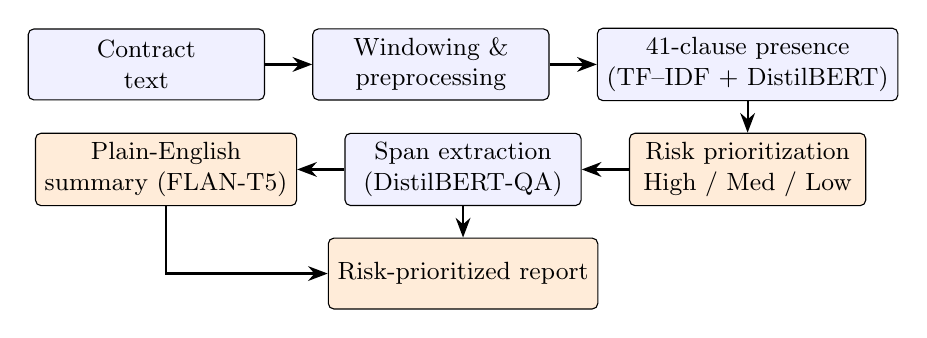
\begin{tikzpicture}[
  node distance=4mm and 6mm,
  stage/.style={draw, rounded corners=2pt, minimum height=9mm, minimum width=30mm,
                align=center, font=\small, fill=blue!6},
  added/.style={stage, fill=orange!15},
  arr/.style={-{Stealth[length=2.5mm]}, thick}
]
\node[stage] (a) {Contract\\text};
\node[stage, right=of a] (b) {Windowing \&\\preprocessing};
\node[stage, right=of b] (c) {41-clause presence\\(TF--IDF + DistilBERT)};
\node[added, below=of c] (d) {Risk prioritization\\High / Med / Low};
\node[stage, left=of d] (e) {Span extraction\\(DistilBERT-QA)};
\node[added, left=of e] (f) {Plain-English\\summary (FLAN-T5)};
\node[added, below=of e] (g) {Risk-prioritized report};
\draw[arr] (a) -- (b);
\draw[arr] (b) -- (c);
\draw[arr] (c) -- (d);
\draw[arr] (d) -- (e);
\draw[arr] (e) -- (f);
\draw[arr] (f.south) |- (g.west);
\draw[arr] (e) -- (g);
\end{tikzpicture}
\end{adjustbox}
\caption{System pipeline}
\label{fig:pipeline}
\end{figure}

\section{Preliminary Design or Design (Model) Specification}
For each step we considered other designs and tested them where we could before choosing one. For finding which clauses are present we compared three designs (a simple word-based model that reads the whole contract, a ``search first, then classify'' transformer, and a transformer that reads the contract in sliding windows) and three ways of combining the simple model with the transformer. We also considered sparse-attention models and rejected them for the reasons in Section~\ref{sec:lit_long}, then measured their cost later (Section~\ref{sec:lfbench}). The design chosen for each step is described below.

\subsection{Stage 2A: Presence Classification}

\subsubsection{A strong baseline first: full-document TF--IDF}
A bag-of-words model has no limit on input length, so a TF--IDF model can read the entire contract, which no windowed transformer can. We built a TF--IDF vocabulary (20{,}000 features, single words and word pairs, sublinear TF, $\text{min\_df}=2$) from the 408 training contracts and trained one balanced logistic-regression classifier per category. Legal writing is very repetitive (``\emph{This Agreement shall be governed by the laws of the State of \ldots}''), so the words alone carry a lot of information. This baseline sets the score every neural model has to beat.

\subsubsection{Measuring the retrieval ceiling, and dropping retrieval}
\label{sec:ceiling}
The obvious way to give a long contract to a transformer is to search first. The text is cut into 2{,}000-character windows that move forward 1{,}500 characters at a time (drawn in Figure~\ref{fig:windows}), each window is scored by its TF--IDF similarity to the category, and the model sees only the best window or windows. The search uses only information that is available when the app runs (the category name or its CUAD question, never the answer), so no answer information leaks in.

Before training anything we measured the search hit-rate: how often the chosen window really contains the clause. Figure~\ref{fig:ceiling} shows how this works and why the result is a hard limit. No model after the search can do better than this number, because a clause in a window the search never picks can never be found. The best search we tried (using the category name and keeping the top 3 windows) reached only 64.0\% (Table~\ref{tab:retrieval}). The CUAD question text did worse than the plain category name, because the questions share so much standard wording that they look almost the same. A recall limit of 0.64 is well below the baseline's recall of 0.81 (and its micro-F1 of 0.775), so a search-first transformer would lose before it was even trained. The measurement took seconds and saved us a wasted training run.

The number needs one note. We measured the limit of word-based search only. Every search in Table~\ref{tab:retrieval} compares windows by shared words, so a clause written without the words of its category name cannot be found even when it is clearly there. A meaning-based search, which turns both the question and each window into vectors, would probably raise the 64.0\% figure, possibly above the baseline, and we did not test one. The fair conclusion is therefore narrow: word-based search sets a limit that is too low to build on. That was enough to move us to the window design in Section~\ref{sec:mil}. Whether meaning-based search could raise the limit far enough to compete is an open question, listed as future work.

\begin{figure}[ht]
\centering
\begin{adjustbox}{max width=\textwidth}
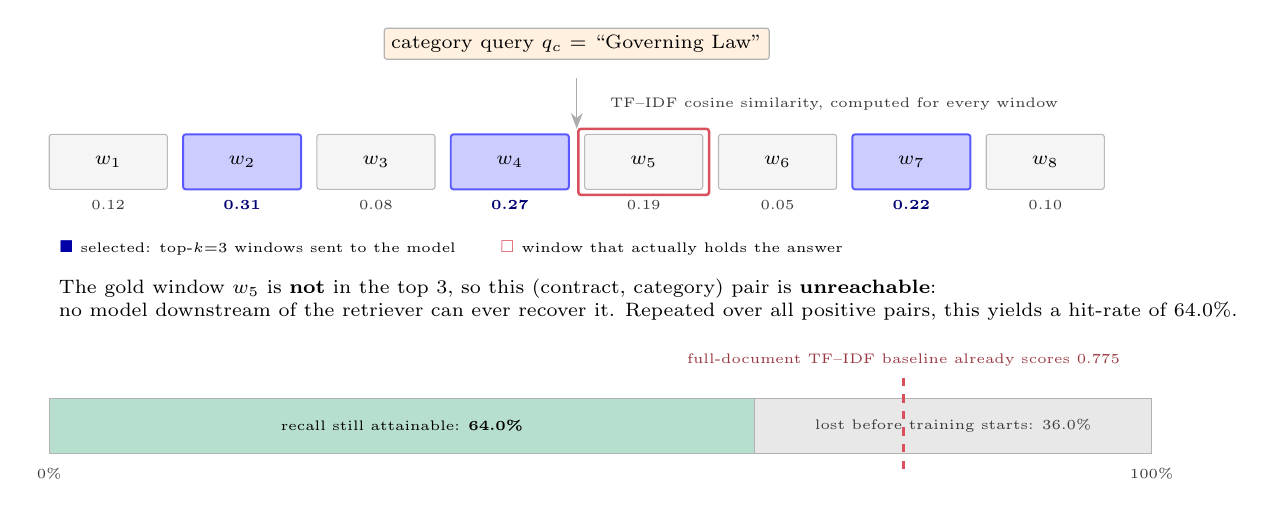
\begin{tikzpicture}[x=1mm, y=1mm, font=\scriptsize,
  wbox/.style={draw=gray!55, fill=gray!8, minimum width=15mm, minimum height=7mm,
               inner sep=0pt, rounded corners=1pt},
  sel/.style={draw=blue!65, fill=blue!20, minimum width=15mm, minimum height=7mm,
              inner sep=0pt, rounded corners=1pt, line width=0.7pt}
]
% ---- query --------------------------------------------------------------
\node[draw=gray!60, fill=orange!12, rounded corners=1pt, inner sep=2.5pt] (q) at (67,22)
  {category query $q_c$ = ``Governing Law''};
\draw[-{Stealth[length=2mm]}, gray!65] (67,17.6) -- (67,11.2);
\node[anchor=west, font=\tiny, text=gray!45!black] at (70,14.4)
  {TF--IDF cosine similarity, computed for every window};

% ---- windows ------------------------------------------------------------
\foreach \i/\x/\s in {1/0/0.12, 3/34/0.08, 5/68/0.19, 6/85/0.05, 8/119/0.10} {
  \node[wbox] (w\i) at (\x+7.5,7) {$w_{\i}$};
  \node[font=\tiny, text=gray!45!black] at (\x+7.5,1.5) {\s};
}
\foreach \i/\x/\s in {2/17/0.31, 4/51/0.27, 7/102/0.22} {
  \node[sel] (w\i) at (\x+7.5,7) {$w_{\i}$};
  \node[font=\tiny, text=blue!45!black] at (\x+7.5,1.5) {\textbf{\s}};
}
% gold-bearing window
\draw[riskhigh, line width=0.9pt, rounded corners=1pt] (67.2,2.8) rectangle (83.8,11.2);

% ---- legend + verdict ---------------------------------------------------
\node[anchor=west, font=\tiny] at (0,-4)
  {\textcolor{blue!65!black}{$\blacksquare$}~selected: top-$k{=}3$ windows sent to the model
   \qquad \textcolor{riskhigh}{$\square$}~window that actually holds the answer};
\node[anchor=west, align=left, font=\scriptsize] at (0,-10.5)
  {The gold window $w_5$ is \textbf{not} in the top~3, so this (contract, category) pair is
   \textbf{unreachable}:\\ no model downstream of the retriever can ever recover it. Repeated over
   all positive pairs, this yields a hit-rate of 64.0\%.};

% ---- ceiling bar --------------------------------------------------------
\fill[risklow!40] (0,-30) rectangle (89.6,-23);
\fill[gray!18]    (89.6,-30) rectangle (140,-23);
\draw[gray!60]    (0,-30) rectangle (140,-23);
\draw[gray!60]    (89.6,-30) -- (89.6,-23);
\node[font=\tiny] at (44.8,-26.5) {recall still attainable: \textbf{64.0\%}};
\node[font=\tiny, text=gray!45!black] at (114.8,-26.5) {lost before training starts: 36.0\%};
\draw[riskhigh, dashed, line width=0.8pt] (108.5,-32) -- (108.5,-20.5);
\node[anchor=south, font=\tiny, text=riskhigh!70!black] at (108.5,-20.2)
  {full-document TF--IDF baseline already scores 0.775};
\node[anchor=north, font=\tiny, text=gray!45!black] at (0,-30.6) {0\%};
\node[anchor=north, font=\tiny, text=gray!45!black] at (140,-30.6) {100\%};
\end{tikzpicture}
\end{adjustbox}
\caption{Retrieval ceiling}
\label{fig:ceiling}
\end{figure}

\begin{table}[ht]
\centering
\caption{Retrieval hit-rates}
\label{tab:retrieval}
\begin{adjustbox}{max width=\textwidth}
\begin{tabular}{lcc}
\toprule
\textbf{Query strategy} & \textbf{Top-$k$} & \textbf{Hit-rate}\\
\midrule
CUAD question text        & 1 & 38.6\%\\
Category name             & 1 & 44.6\%\\
\textbf{Category name}    & \textbf{3} & \textbf{64.0\%}\\
Name + question           & 3 & 61.5\%\\
\bottomrule
\end{tabular}
\end{adjustbox}

{\footnotesize\singlespacing \emph{Note.} The hit-rate is the recall ceiling a retrieval-based design would impose.\par}
\end{table}

\subsubsection{Sliding-window max-pooling (multiple-instance learning)}
\label{sec:mil}
To remove this limit we trained a window-level classifier instead. Given a pair (category question, window), it predicts whether that window contains a clause of that category. Figure~\ref{fig:windows} shows how the windows are made. A 2{,}000-character window that moves forward 1{,}500 characters at a time leaves a 500-character overlap between neighbouring windows. The typical (median) clause is 196 characters long (Section~\ref{sec:eda}), much shorter than the overlap, so every clause fits completely inside at least one window and none falls between two.

\begin{figure}[ht]
\centering
\begin{adjustbox}{max width=\textwidth}
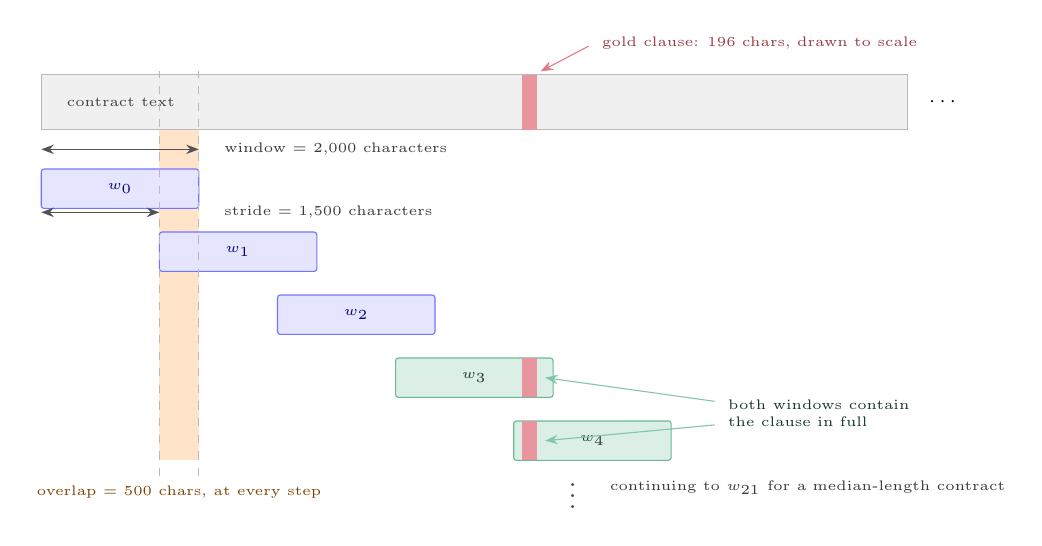
\begin{tikzpicture}[x=1mm, y=1mm, font=\scriptsize,
  dim/.style={{Stealth[length=1.6mm]}-{Stealth[length=1.6mm]}, gray!65!black, line width=0.5pt},
  win/.style={draw=blue!55, fill=blue!10, rounded corners=1pt},
  poswin/.style={draw=risklow!85, fill=risklow!20, rounded corners=1pt}]

% ---- overlap band (behind everything) -----------------------------------
\fill[orange!30, opacity=0.7] (15,-42) rectangle (20,0);

% ---- the document -------------------------------------------------------
\fill[gray!12] (0,0) rectangle (110,7);
\draw[gray!55] (0,0) rectangle (110,7);
\fill[riskhigh!60] (61,0) rectangle (63,7);
\node[anchor=west, text=gray!50!black, font=\tiny] at (2,3.5) {contract text};
\node[anchor=west] at (111.5,3.5) {$\cdots$};
\node[anchor=west, text=riskhigh!70!black, font=\tiny] at (70,11)
  {gold clause: 196 chars, drawn to scale};
\draw[riskhigh!75, -{Stealth[length=1.6mm]}] (69.5,10.6) -- (63.4,7.4);

% ---- staircase of windows ----------------------------------------------
\foreach \i/\y in {0/-5, 1/-13, 2/-21} {
  \draw[win] (15*\i,\y-5) rectangle (15*\i+20,\y);
  \node[text=blue!45!black, font=\tiny] at (15*\i+10,\y-2.5) {$w_{\i}$};
}
\foreach \i/\y in {3/-29, 4/-37} {
  \draw[poswin] (15*\i,\y-5) rectangle (15*\i+20,\y);
  \node[text=risklow!35!black, font=\tiny] at (15*\i+10,\y-2.5) {$w_{\i}$};
  \fill[riskhigh!60] (61,\y-5) rectangle (63,\y);
}
\node[anchor=west, text=risklow!30!black, font=\tiny, align=left] at (86,-36)
  {both windows contain\\the clause in full};
\draw[risklow!70, -{Stealth[length=1.6mm]}] (85.5,-34.5) -- (64,-31.5);
\draw[risklow!70, -{Stealth[length=1.6mm]}] (85.5,-37.5) -- (64,-39.5);

% ---- dimensions ---------------------------------------------------------
\draw[dim] (0,-2.5) -- (20,-2.5);
\node[anchor=west, font=\tiny, text=gray!45!black] at (22,-2.5)
  {window $=$ 2{,}000 characters};
\draw[dim] (0,-10.5) -- (15,-10.5);
\node[anchor=west, font=\tiny, text=gray!45!black] at (22,-10.5)
  {stride $=$ 1{,}500 characters};
\draw[gray!55, dashed, line width=0.4pt] (15,-44) -- (15,7.5);
\draw[gray!55, dashed, line width=0.4pt] (20,-44) -- (20,7.5);
\node[anchor=north, align=center, font=\tiny, text=orange!50!black] at (17.5,-44)
  {overlap $=$ 500 chars, at every step};
\node[font=\normalsize, text=gray!55!black] at (67.5,-45.5) {$\vdots$};
\node[anchor=west, font=\tiny, text=gray!45!black] at (71,-45.5)
  {continuing to $w_{21}$ for a median-length contract};
\end{tikzpicture}
\end{adjustbox}
\caption{Sliding-window generation}
\label{fig:windows}
\end{figure}

The training labels come from the marked character positions. Any window that contains a marked clause is positive, and for each (contract, category) pair we also take two random negative windows. This is normal supervised learning and does not leak answers: the labels only set the training targets, they never enter the model's input, and nothing from the answers is used when the app runs. The 408 training contracts give 53{,}662 window examples (39.2\% positive).

When the app runs, the model scores every window of the contract, and the answer for the whole contract is the highest window score. This is the multiple-instance learning rule, shown in Figure~\ref{fig:mil}: the document is a bag of windows, the bag is positive if any window is positive, and taking the $\max$ does exactly that. Because the windows cover the whole document with overlap, every clause can be reached and the search limit disappears. The cost is precision, and Figure~\ref{fig:mil} also shows why. The maximum is taken over every window, so one wrong window anywhere marks the whole contract as positive. A typical contract has 22 windows (the median; the mean is 35), so the chance that some window passes the 0.5 threshold by mistake grows with length, and long contracts give more false alarms than short ones whatever they contain.

\begin{figure}[ht]
\centering
\begin{adjustbox}{max width=\textwidth}
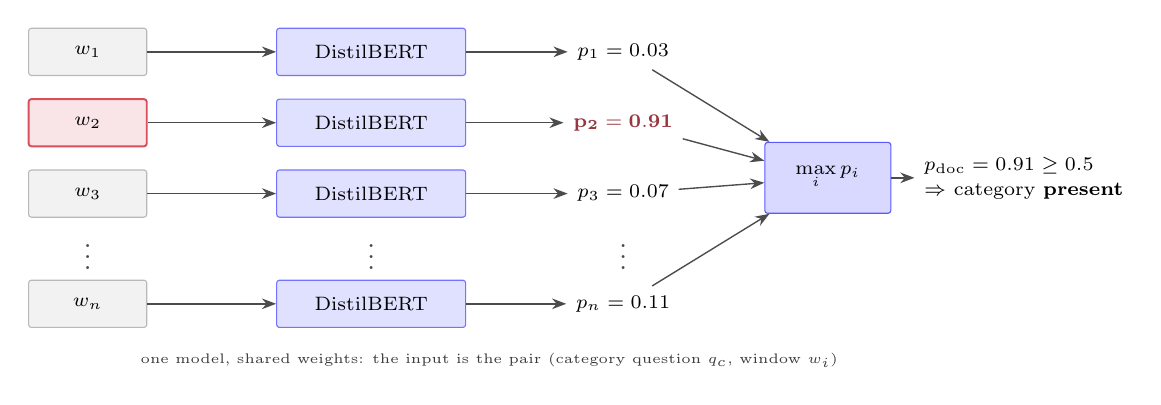
\begin{tikzpicture}[x=1mm, y=1mm, font=\scriptsize,
  win/.style={draw=gray!55, fill=gray!10, rounded corners=1pt,
              minimum width=15mm, minimum height=6mm, inner sep=0pt},
  hot/.style={draw=riskhigh, fill=riskhigh!15, rounded corners=1pt,
              minimum width=15mm, minimum height=6mm, inner sep=0pt, line width=0.7pt},
  enc/.style={draw=blue!55, fill=blue!12, rounded corners=1pt,
              minimum width=24mm, minimum height=6mm, inner sep=0pt},
  arr/.style={-{Stealth[length=1.8mm]}, gray!60!black, line width=0.5pt}
]
% rows: w1, w2 (firing), w3, vdots, wn
\node[win] (w1) at (9,0)    {$w_1$};
\node[hot] (w2) at (9,-9)   {$w_2$};
\node[win] (w3) at (9,-18)  {$w_3$};
\node[font=\normalsize, text=gray!55!black] at (9,-25) {$\vdots$};
\node[win] (wn) at (9,-32)  {$w_n$};

\node[enc] (e1) at (45,0)   {DistilBERT};
\node[enc] (e2) at (45,-9)  {DistilBERT};
\node[enc] (e3) at (45,-18) {DistilBERT};
\node[font=\normalsize, text=gray!55!black] at (45,-25) {$\vdots$};
\node[enc] (en) at (45,-32) {DistilBERT};

\node (p1) at (77,0)   {$p_1 = 0.03$};
\node[text=riskhigh!70!black] (p2) at (77,-9) {$\mathbf{p_2 = 0.91}$};
\node (p3) at (77,-18) {$p_3 = 0.07$};
\node[font=\normalsize, text=gray!55!black] at (77,-25) {$\vdots$};
\node (pn) at (77,-32) {$p_n = 0.11$};

\foreach \a/\b in {w1/e1, w2/e2, w3/e3, wn/en} \draw[arr] (\a) -- (\b);
\foreach \a/\b in {e1/p1, e2/p2, e3/p3, en/pn} \draw[arr] (\a) -- (\b);

% max node
\node[draw=blue!65, fill=blue!15, rounded corners=1pt, minimum width=16mm,
      minimum height=9mm, inner sep=1pt, align=center] (mx) at (103,-16)
      {$\max\limits_i p_i$};
\foreach \p in {p1,p2,p3,pn} \draw[arr] (\p) -- (mx);

\node[anchor=west, align=left] (out) at (114,-16)
  {$p_{\text{doc}} = 0.91 \geq 0.5$\\[1pt] $\Rightarrow$ category \textbf{present}};
\draw[arr] (mx) -- (out);

% annotations
\node[anchor=north, align=center, font=\tiny, text=gray!45!black] at (60,-37)
  {one model, shared weights: the input is the pair (category question $q_c$, window $w_i$)};
\end{tikzpicture}
\end{adjustbox}
\caption{Multiple-instance max-pooling}
\label{fig:mil}
\end{figure}

\subsubsection{The conjunctive ensemble}
Compared category by category, the two models turned out to complement each other. The transformer does better where meaning matters (for example \emph{No-Solicit of Employees} and \emph{Liquidated Damages}), and the simple model does better on categories with clear keywords. We combine them with rules that have no settings to tune: AND (the $\min$ of the two scores), OR (the $\max$) and AVG (the average). We chose such rules on purpose so that nothing can be fitted to the test set. Figure~\ref{fig:ensemble_rule} shows the decision. The AND rule reports a clause only when both models agree, which removes many false alarms. For a wrong detection to survive, both models must make the same mistake on the same contract and category, and their mistakes are mostly independent. This wins back the precision that taking the maximum loses.

\begin{figure}[ht]
\centering
\begin{adjustbox}{max width=\textwidth}
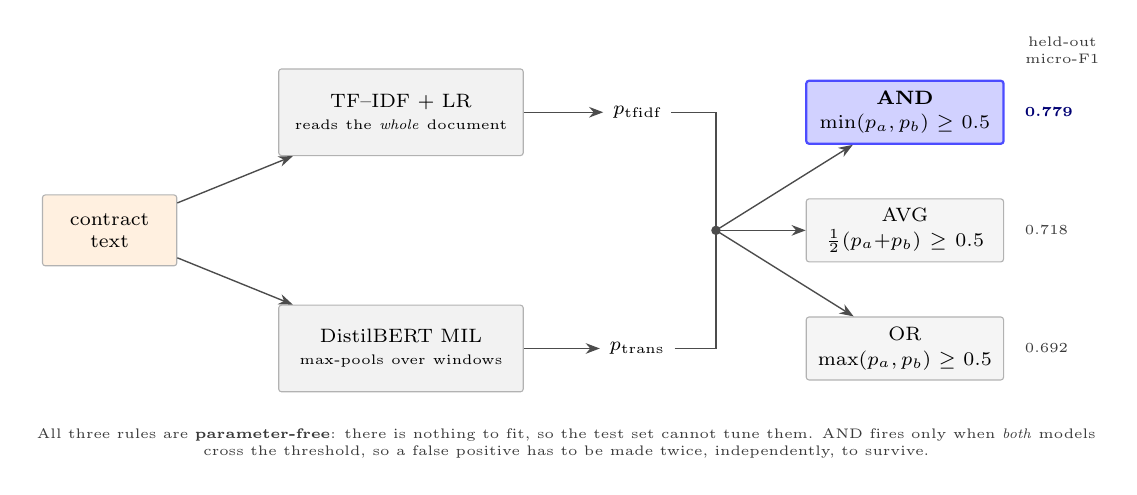
\begin{tikzpicture}[x=1mm, y=1mm, font=\scriptsize,
  mod/.style={draw=gray!60, fill=gray!10, rounded corners=1pt, text width=30mm,
              align=center, minimum height=11mm, inner sep=1.5pt},
  rule/.style={draw=gray!60, fill=gray!8, rounded corners=1pt, text width=24mm,
               align=center, minimum height=8mm, inner sep=1.5pt},
  pick/.style={rule, draw=blue!70, fill=blue!18, line width=0.8pt},
  arr/.style={-{Stealth[length=1.8mm]}, gray!60!black, line width=0.5pt}
]
\node[draw=gray!60, fill=orange!12, rounded corners=1pt, text width=16mm, align=center,
      minimum height=9mm, inner sep=1.5pt] (doc) at (9,0) {contract\\text};

\node[mod] (bl) at (46,15) {TF--IDF $+$ LR\\{\tiny reads the \emph{whole} document}};
\node[mod] (tr) at (46,-15) {DistilBERT MIL\\{\tiny max-pools over windows}};
\draw[arr] (doc) -- (bl);
\draw[arr] (doc) -- (tr);

\node (pa) at (76,15)  {$p_{\text{tfidf}}$};
\node (pb) at (76,-15) {$p_{\text{trans}}$};
\draw[arr] (bl) -- (pa);
\draw[arr] (tr) -- (pb);

\coordinate (j) at (86,0);
\draw[gray!60!black, line width=0.5pt] (pa) -- (86,15) -- (j);
\draw[gray!60!black, line width=0.5pt] (pb) -- (86,-15) -- (j);
\fill[gray!60!black] (j) circle (0.6mm);

\node[pick] (rand) at (110,15)  {\textbf{AND}\\[1pt]$\min(p_a,p_b) \geq 0.5$};
\node[rule] (ravg) at (110,0)   {AVG\\[1pt]$\tfrac{1}{2}(p_a{+}p_b) \geq 0.5$};
\node[rule] (ror)  at (110,-15) {OR\\[1pt]$\max(p_a,p_b) \geq 0.5$};
\foreach \r in {rand,ravg,ror} \draw[arr] (j) -- (\r);

\node[anchor=west, font=\tiny, text=blue!45!black] at (124,15) {\textbf{0.779}};
\node[anchor=west, font=\tiny, text=gray!45!black]  at (124,0)  {0.718};
\node[anchor=west, font=\tiny, text=gray!45!black]  at (124,-15){0.692};
\node[anchor=south, font=\tiny, text=gray!45!black, align=center] at (130,20)
  {held-out\\micro-F1};

\node[anchor=north, align=center, font=\tiny, text=gray!45!black] at (67,-24)
  {All three rules are \textbf{parameter-free}: there is nothing to fit, so the test set cannot tune them.
   AND fires only when \emph{both} models\\ cross the threshold, so a false positive has to be made
   twice, independently, to survive.};
\end{tikzpicture}
\end{adjustbox}
\caption{Ensemble rules}
\label{fig:ensemble_rule}
\end{figure}
\subsection{Stage 2B: Span Extraction}
\label{sec:spanmethod}
This step needs the transformer, because a bag-of-words model cannot point to positions in the text. We fine-tune \texttt{DistilBertForQuestionAnswering}: the input is (CUAD question, window text), and the model predicts where the answer starts and ends. The character positions in \texttt{CUAD\_v1.json} are turned into token positions with the tokenizer's offset mapping.

The project uses two window sizes, and mixing them up makes the design look inconsistent. The 2{,}000-character window of Section~\ref{sec:mil} is a presence window. It covers the document in order, because at that point we do not know where anything is. The window used here is a focus window, 1{,}200 characters long and placed around the marked answer so that the answer starts about 150 characters in. Figure~\ref{fig:focus} draws the two at the same scale. The smaller, centred window has a simple technical purpose: it keeps the answer inside the model's 320-token limit. With a 2{,}000-character window an answer near the end could be cut off, and the model would be trained on an example with the answer missing. This step also has no length limit at all, since it only searches inside a window that the presence step has already marked as relevant.

\begin{figure}[ht]
\centering
\begin{adjustbox}{max width=\textwidth}
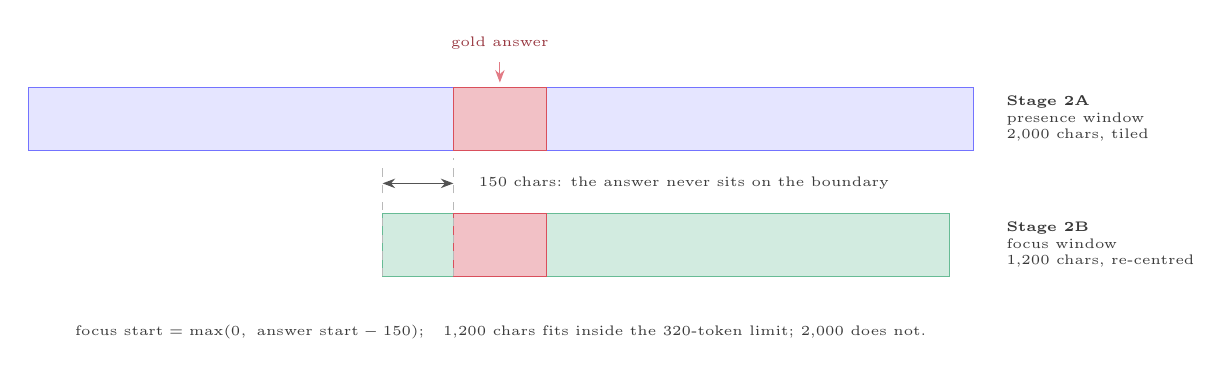
\begin{tikzpicture}[x=1mm, y=1mm, font=\scriptsize,
  dim/.style={{Stealth[length=1.6mm]}-{Stealth[length=1.6mm]}, gray!65!black, line width=0.5pt}]

% ---- presence window (Stage 2A) ----------------------------------------
\fill[blue!10] (0,0) rectangle (120,8);
\draw[blue!55] (0,0) rectangle (120,8);
\fill[riskhigh!35] (54,0) rectangle (65.8,8);
\draw[riskhigh]    (54,0) rectangle (65.8,8);
\node[anchor=west, align=left, font=\tiny, text=gray!45!black] at (123,4)
  {\textbf{Stage 2A}\\presence window\\2{,}000 chars, tiled};
\node[anchor=south, font=\tiny, text=riskhigh!70!black] at (59.9,11.6) {gold answer};
\draw[riskhigh!75, -{Stealth[length=1.6mm]}] (59.9,11.2) -- (59.9,8.6);

% ---- focus window (Stage 2B) -------------------------------------------
\fill[risklow!25] (45,-16) rectangle (117,-8);
\draw[risklow!85] (45,-16) rectangle (117,-8);
\fill[riskhigh!35] (54,-16) rectangle (65.8,-8);
\draw[riskhigh]    (54,-16) rectangle (65.8,-8);
\node[anchor=west, align=left, font=\tiny, text=gray!45!black] at (123,-12)
  {\textbf{Stage 2B}\\focus window\\1{,}200 chars, re-centred};

% ---- alignment guides + offset -----------------------------------------
\draw[gray!55, dashed, thin] (45,-16) -- (45,-2);
\draw[gray!55, dashed, thin] (54,-16) -- (54,-1);
\draw[dim] (45,-4.2) -- (54,-4.2);
\node[anchor=west, font=\tiny, text=gray!45!black] at (56,-4.2)
  {150 chars: the answer never sits on the boundary};

% ---- footer ------------------------------------------------------------
\node[anchor=north, align=center, font=\tiny, text=gray!45!black] at (60,-21)
  {$\text{focus start} = \max(0,\ \text{answer start} - 150)$;\quad
   1{,}200 chars fits inside the 320-token limit; 2{,}000 does not.};
\end{tikzpicture}
\end{adjustbox}
\caption{Presence vs.\ focus window}
\label{fig:focus}
\end{figure}
\subsection{Stage 1: Plain-Language Summarization}
\label{sec:summmethod}
CUAD gives us clauses but no plain-English versions to learn from, so we wrote our own: 41 template sentences, one carefully written one-sentence summary for each category, from the weaker party's side. For \emph{Anti-Assignment}, for example, the template is ``You cannot transfer this contract to someone else without permission.'' Each training clause is paired with its category's template, which gives 11{,}156 training pairs, and FLAN-T5-small is fine-tuned on the prompt ``\texttt{summarize in plain English: <clause>}''.

We test the summarizer in two ways: with ROUGE-L, and by comparing the fine-tuned model with the original model on the same clauses. We need both. With only 41 different target sentences, a model can get a high ROUGE score by recognising the category and copying its template word for word, without summarizing anything. Chapter~5 shows that this is exactly what happens.
\subsection{Category-Level Risk Prioritization}
\label{sec:risk}
The name of this layer limits what we can claim. The system does not read a clause and judge how dangerous that clause is. It finds which of the 41 categories a contract contains and gives each category a fixed level. These are different tasks, and treating them as one would greatly overstate the system. Our layer says ``\emph{contracts with a non-compete deserve attention}'' and never says ``\emph{this non-compete is unusually harsh}''. Throughout this report we therefore call it category-level risk prioritization.

\subsubsection{Assignment criteria}
\label{sec:riskcriteria}
We wrote down the rules we used so that a reader, or a reviewing lawyer, can disagree with a particular level for a particular reason. Each category was scored on five points, from the weaker party's side:

\begin{enumerate}[itemsep=3pt]
  \item \textbf{Money at risk.} Can this clause cost money, and is there a limit? Having no limit is the strongest single sign of High risk.
  \item \textbf{Cannot be undone.} If the clause takes effect, can the situation be reversed? Losing ownership of intellectual property or giving a permanent licence cannot be undone later; a notice period can.
  \item \textbf{Limits on future freedom.} Does the clause limit what the party can do \emph{after} the contract, or outside it, such as who it may work for, sell to or hire?
  \item \textbf{One-sided.} Does the duty fall on only one side? A shared duty of confidentiality is less dangerous than a one-way indemnity with the same wording.
  \item \textbf{How long it lasts.} Does the duty continue after the contract ends?
\end{enumerate}

The rule we used is this. A category is High if it has no money limit (point~1), cannot be undone (point~2), or limits freedom after the contract (point~3). It is Low if it only gives information (it records a fact such as a date, a name or the governing law, or gives a benefit) and scores on none of the five points. Everything else is Medium: a real duty, but limited and reversible. This is why \emph{Cap on Liability} is Medium even though it sounds protective (it limits how much you can recover, which may not cover a real loss), and why \emph{Governing Law} is Low even though it matters in a court case (it is a fact about the contract and puts no one-sided duty on the signer).

The eight High categories fall into three groups, each based on a different point: money you could owe without limit (\emph{Uncapped Liability}, \emph{Liquidated Damages}, \emph{Minimum Commitment}, \emph{Most Favored Nation}); something you cannot get back (\emph{IP Ownership Assignment}, \emph{Irrevocable/Perpetual License}); and your freedom to earn later (\emph{Non-Compete}, \emph{Exclusivity}). The full table with reasons is in Appendix~\ref{app:taxonomy}, and Figure~\ref{fig:riskdist} shows how the categories are spread across the levels.

\subsubsection{Who is the ``weaker party''?}
\label{sec:weaker}
The risk table depends on this phrase, which can mean different things. The weaker party is not always the same role. In a distribution contract it may be the distributor, in a licence the licensee, and in a franchise the franchisee. In a balanced contract between equals there may be no weaker party at all.

We defined it as the party with less power over how the contract was written, which in CUAD is usually the party that did not write it. Where the category alone did not make this clear, we scored from the side of the party who carries the duty: \emph{Non-Compete} from the side that is restricted, \emph{Audit Rights} from the side that is audited, and \emph{License Grant} from the side that receives the licence. This rule of thumb has a known weakness. A clause that is High-risk for one side often protects the other, so the same badge is not equally useful to a licensor and a licensee. A system that judged each clause on its own could work out the side from the clause text. Ours cannot, so it assumes the user is the side with less power, and the app states this in the notice shown above every analysis.

\subsubsection{Why a lookup table rather than a learned score}
The risk table is a simple lookup, which we chose on purpose. It can be checked line by line, its reasoning is written down for each category, and it cannot change silently between versions. The cost is the limit named at the start of this section: it cannot tell a \$10{,}000 liability limit from a \$10{,}000{,}000 one. Section~\ref{sec:riskeval} measures a second cost we did not expect. Because the levels are fixed per category, the system's mistakes depend entirely on which categories it finds well, and the High-risk categories turn out to be among those it finds worst.


\subsubsection{Provenance and validation status of the taxonomy}
\label{sec:taxvalid}
The risk table is the main thing this project adds to CUAD, and it also has the weakest evidence behind it, so we state where it comes from.

The three of us set all 41 levels. We are computer science students, not lawyers. We judged each category by its effect on the weaker party (can this clause cost you unlimited money, take away something you cannot get back, or limit what you can do later?) and compared our levels with the CUAD category descriptions. The levels rest only on our own judgement, and no legal professional has reviewed them.

Every other part of this project is measured against answers marked by experts, and this part is measured against nothing. It also affects the user most directly, since the level decides what Clausify tells a signer to worry about first. If we marked a category Medium that a lawyer would mark High, the app fails silently: the warning never appears.

The basic check is a review by someone with legal training. The reviewer gets the 41 categories with our level and reason, says whether they agree with each one, and we report the number of disagreements, whatever it is. We have prepared a review sheet for this (\texttt{review/risk\_taxonomy\_review\_sheet.csv} in the repository, with one row per category and columns for the reviewer's own level and comments). It takes a reviewer about half an hour.

One reviewer would give a basic check, and two or three reviewing separately would give a stronger one. Simple percentage agreement is a poor measure for this table because the levels are uneven: 22 of the 41 categories are Medium, so a reviewer who answered ``Medium'' every time would agree 54\% of the time while adding no information. Agreement corrected for chance (Cohen's $\kappa$ for two reviewers, Fleiss' $\kappa$ for three or more) removes this problem, and that is what we would report. The repository includes \texttt{review/agreement.py}, which reads the completed sheets and prints each reviewer's agreement, both kappa values and the categories in dispute. The analysis is fixed in advance, so the results cannot shape it.

\emph{At the time of writing this review has not been done, and no number from it is reported anywhere in this project.} Until then, every level has a written reason that can be argued with line by line, but no qualified person has checked any of them.
%% ==================================================================
%% TODO BEFORE FINAL SUBMISSION -- REPLACE THE ITALIC PARAGRAPH ABOVE
%%
%% Send review/REVIEWER_REQUEST.md + risk_taxonomy_review_sheet.csv to a
%% law student or practitioner. Then delete the italic sentence above and
%% paste ONE of the following, filling in the numbers.
%%
%% --- IF TWO OR MORE REVIEWERS COMPLETED THE SHEET -----------------
%% Run: python review/agreement.py reviewer1.csv reviewer2.csv
%%
%% "The 41 assignments were reviewed independently by <N> reviewers
%%  (<roles>) in <month year>. Agreement with our levels was <X>% and <Y>%;
%%  Cohen's kappa against our taxonomy was <k1> and <k2>, and reviewer-to-
%%  reviewer agreement was <k3> (<interpretation>). The <M> disputed
%%  categories were <list>. We adopted <K> of these changes; Appendix A
%%  reflects the revised levels. We report the disagreements we did not
%%  adopt as well, with our reason in each case."
%%
%% --- IF ONLY ONE REVIEWER WAS AVAILABLE ---------------------------
%% Run: python review/agreement.py reviewer1.csv
%%
%% "The 41 assignments were reviewed by <name/role> in <month year>. The
%%  reviewer agreed with <X> of 41 (<Y>%); the <M> disputed categories were
%%  <list>, of which we adopted <K>. Only one reviewer was available in the
%%  time before submission, so inter-rater statistics (Cohen's or Fleiss'
%%  kappa) could not be computed and no chance-corrected agreement figure is
%%  reported. Raw agreement on a three-level scale where 22 of 41 categories
%%  are Medium should be read with that in mind."
%%
%% Report the disagreements WHATEVER they are. A low agreement figure,
%% honestly reported, is a stronger report than no figure at all.
%% ==================================================================

\begin{figure}[ht]
\centering
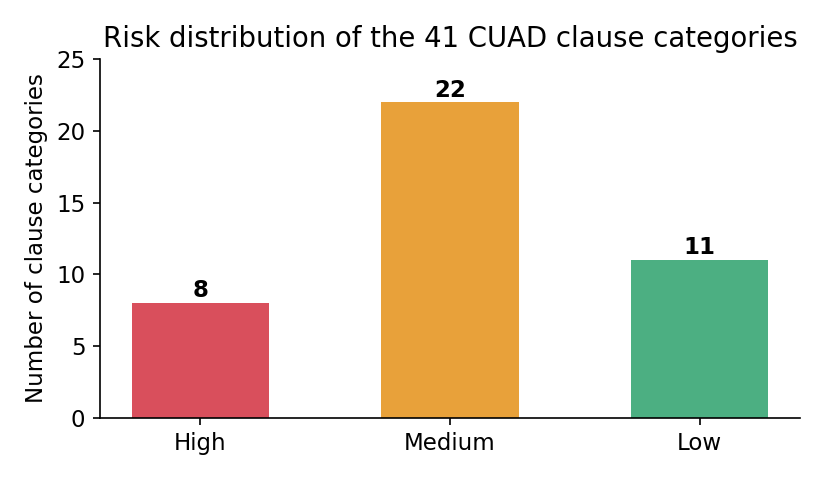
\includegraphics[width=0.62\textwidth]{risk_distribution.png}
\caption{Risk-level distribution}
\label{fig:riskdist}
\end{figure}
\subsection{Avoiding Data Leakage}
\label{sec:leakage}
With such a small dataset, data leakage is the easiest way to fool ourselves, so we followed one rule throughout: \emph{the answers may be used to create training targets, but never to shape what a model reads or what is chosen when the app runs}. In practice the split is by contract, searches use only the category or its question, the marked answer positions label training windows but never build inputs or choose windows when the app runs, and the ensemble rules have no settings for the test set to tune.

Figure~\ref{fig:focus} shows the one place where the rule seems to be broken. The focus window is placed using the marked answer position, which is part of the answer. In training this is normal supervised learning, because it decides which text becomes a training example. In the real system there is no marked answer, and the span step reads the window chosen by the presence step. The separate span test in Section~\ref{sec:span} is the exception. It builds each test example with the same centred focus window, so it measures extraction when the position of the answer is already known, and its score is a best case that the real system cannot reach. The realistic number comes from the start-to-finish test in Section~\ref{sec:e2e}, which never uses the marked answer position.

\section{Data Collection}
\label{sec:datasource}
All experiments use the official CUAD release from The Atticus Project, downloaded from the Hugging Face hub (\texttt{theatticusproject/cuad}). The default \texttt{load\_dataset()} option gives only the 511 original contract PDFs, which cannot be used for training. The marked data sits in two files in the repository, and each has a different job in our system:
\begin{itemize}[itemsep=2pt]
  \item \texttt{master\_clauses.csv}: a wide table with 83 columns and one row per contract, which we used to explore the data and build labels;
  \item \texttt{CUAD\_v1.json}: the SQuAD-format file with the full contract text and the character positions of every answer, which we used to train the span model and to read whole contracts.
\end{itemize}

\subsection{Data Cleaning}
Experts prepared the CUAD files, so cleaning meant fixing format problems; the values themselves were sound. We handled four problems:
\begin{itemize}[itemsep=2pt]
  \item Empty cells. Clause-text cells that are empty (\texttt{NaN}) are treated as an empty list, which means the category is absent.
  \item Badly formed lists. Each clause-text cell holds a Python list written as text. A cell that cannot be read as a list is kept as one clause instead of being thrown away, and blank entries are removed from every list.
  \item Inconsistent column names. The column name \texttt{Notice Period To Terminate Renewal- Answer} contains an extra space that breaks matching by name, so columns were paired by position instead (Section~\ref{sec:datasource}).
  \item Empty answers in the JSON file. Answers that are empty after removing spaces are ignored when building the span-training examples and the answer lists.
\end{itemize}
We removed no unusual values. Very long contracts are real and were kept, because handling length is exactly what the method must do.

\subsection{Data Transformation}
The CSV is wide: 41 categories $\times$ (a clause-text column plus an answer column), with a file-name column at the front. Turning it into a long table with one row per (contract, category) needed two decisions that were not obvious at first:

We paired columns by position. The column name \texttt{Notice Period To Terminate Renewal- Answer} contains an extra space, which silently breaks any matching of a category column to its answer column by name. Pairing by position (clause text in odd columns, answer in even columns) is immune to such typos.

We decided presence from the clause-text list and ignored the Yes/No answer. Each clause-text cell holds a Python list written as text, either \texttt{'[]'} or \texttt{"['clause', ...]"}, and a category is present when this list is not empty. The rule works the same way for the eight categories (dates, party names) whose answer column holds a value instead of Yes/No, and it also gives us the clause text directly.

This gives $510 \times 41 = 20{,}910$ labelled (contract, category) rows, of which 32.1\% are positive.

Three more steps prepare the data for the models. Every contract is cut into 2{,}000-character windows that move forward 1{,}500 characters at a time, so neighbouring windows overlap by 500 characters, more than a typical clause, and no clause falls between two windows. For the span model, CUAD's character positions are turned into start and end token positions with the tokenizer's offset mapping, inside a 1{,}200-character focus window around each answer so that it fits in 320 tokens. For the baseline, each whole contract becomes a TF--IDF vector of single words and word pairs with sublinear term frequency. Category labels stay simple present/absent values, and no other scaling is needed beyond what TF--IDF does.

\subsection{Data Integration}
The two CUAD files complement each other. \texttt{master\_clauses.csv} gives one row per contract with the clause lists we used to explore the data and build labels, and \texttt{CUAD\_v1.json} gives the full contract text, the 41 category questions and the character positions of every marked clause. All the modelling uses the JSON file: presence labels, answers and contract texts come from it, matched by contract title and by the category name taken from each question ID. We used the CSV to explore the data and to double-check how often each category appears. The split by contract is computed once over the 510 contract titles and applied the same way to every table made from the data.

\subsection{Data Reduction}
We reduced the data only to keep training possible on a laptop and to balance the classes, and never threw away information the app needs when it runs:
\begin{itemize}[itemsep=2pt]
  \item Vocabulary limit for the baseline: the TF--IDF vocabulary keeps only the 20{,}000 most common single words and word pairs that appear in at least two contracts.
  \item Fewer negative examples: for window-level training, every positive window is kept, but only two negative windows are taken for each (contract, category) pair, giving 53{,}662 window examples with 39.2\% positives.
  \item Training on a sample: the presence model was trained on a balanced sample of 24{,}000 windows, the span model on 8{,}000 of 11{,}156 examples and the summarizer on 4{,}000 of 11{,}156 pairs. Section~\ref{sec:budget} tests whether training the presence model on a sample hurt it.
\end{itemize}

\subsection{Summary of Preprocessed Data}
\label{sec:eda}
Four features of the data shaped the design decisions that followed:

\begin{enumerate}[itemsep=2pt]
  \item Very uneven categories. How often a category appears ranges from \emph{Document Name} at 100\% and \emph{Parties} at 99.8\% down to \emph{Source Code Escrow} at 2.5\% and \emph{Price Restrictions} at 2.9\%. The median category appears in about 23\% of contracts.
  \item Almost no examples of the rarest categories. \emph{Source Code Escrow} appears in only 13 contracts in the whole dataset. No model can learn such categories reliably, and their individual scores are mostly noise, which we keep in mind throughout the results chapter.
  \item Long contracts. The median is 33{,}143 characters (about 5{,}000 words) and the maximum is 338{,}211 characters. The median is about 16$\times$ what a transformer can read at once (about 2{,}000 characters), and the longest is about 170$\times$, which makes length the central modelling problem of the project.
  \item Short clauses. The median marked clause is 196 characters (90th percentile 587, 99th percentile 1{,}330). A clause easily fits inside one window; the hard part is finding it in a very long document.
\end{enumerate}

The 510 contracts are the whole dataset. Marking them reportedly cost about \$2M of lawyers' time, so more cannot easily be added. This has three effects: we must start from pre-trained models, over-fitting is the main danger and so all our conclusions rest on test-set numbers, and the train/test split must be made by contract.

\subsubsection{The 80/20 Train/Test Split}
As our supervisor asked, we split the dataset 80/20 by contract. Each whole contract goes to one side or the other, so no clause from a training contract can appear in the test set. The split uses a fixed random seed (42), and all three models use exactly the same split, so ``test'' always means the same 102 unseen contracts. Table~\ref{tab:split} summarizes the split, and the almost equal share of positives on both sides shows it is balanced. We saved the two sides as \texttt{data/train\_80.csv} and \texttt{data/test\_20.csv} so the split itself can be repeated.

\begin{table}[ht]
\centering
\caption{Train/test split}
\label{tab:split}
\begin{adjustbox}{max width=\textwidth}
\begin{tabular}{lrrr}
\toprule
 & \textbf{Contracts} & \textbf{(Contract, category) rows} & \textbf{Positive rate}\\
\midrule
Train (80\%) & 408 & 16{,}728 & 32.0\%\\
Test (20\%)  & 102 & 4{,}182  & 32.2\%\\
\midrule
Total        & 510 & 20{,}910 & 32.1\%\\
\bottomrule
\end{tabular}
\end{adjustbox}
\end{table}

The overall share of positives in Table~\ref{tab:split} is almost the same on both sides (32.0\% vs.\ 32.2\%). One pair of numbers can still hide a badly uneven split, since the two sides can match overall and differ a lot category by category, so Figure~\ref{fig:splitdist} compares them for all 41 categories at once. They match closely (Pearson $r = 0.986$, average difference 3.4 percentage points). The clear exception is \emph{Termination For Convenience}, which appears in 47.1\% of test contracts but only 33.1\% of training contracts, a 14.0-point gap. The other differences are all in the rarest categories, where moving one or two contracts changes the percentage by several points. The split was made once at random and never changed to look better, so we report these gaps as they are. They matter in Chapter~5, because a category that is more common in the test set counts more in the micro-averaged score than its training frequency would suggest.

\begin{figure}[ht]
\centering
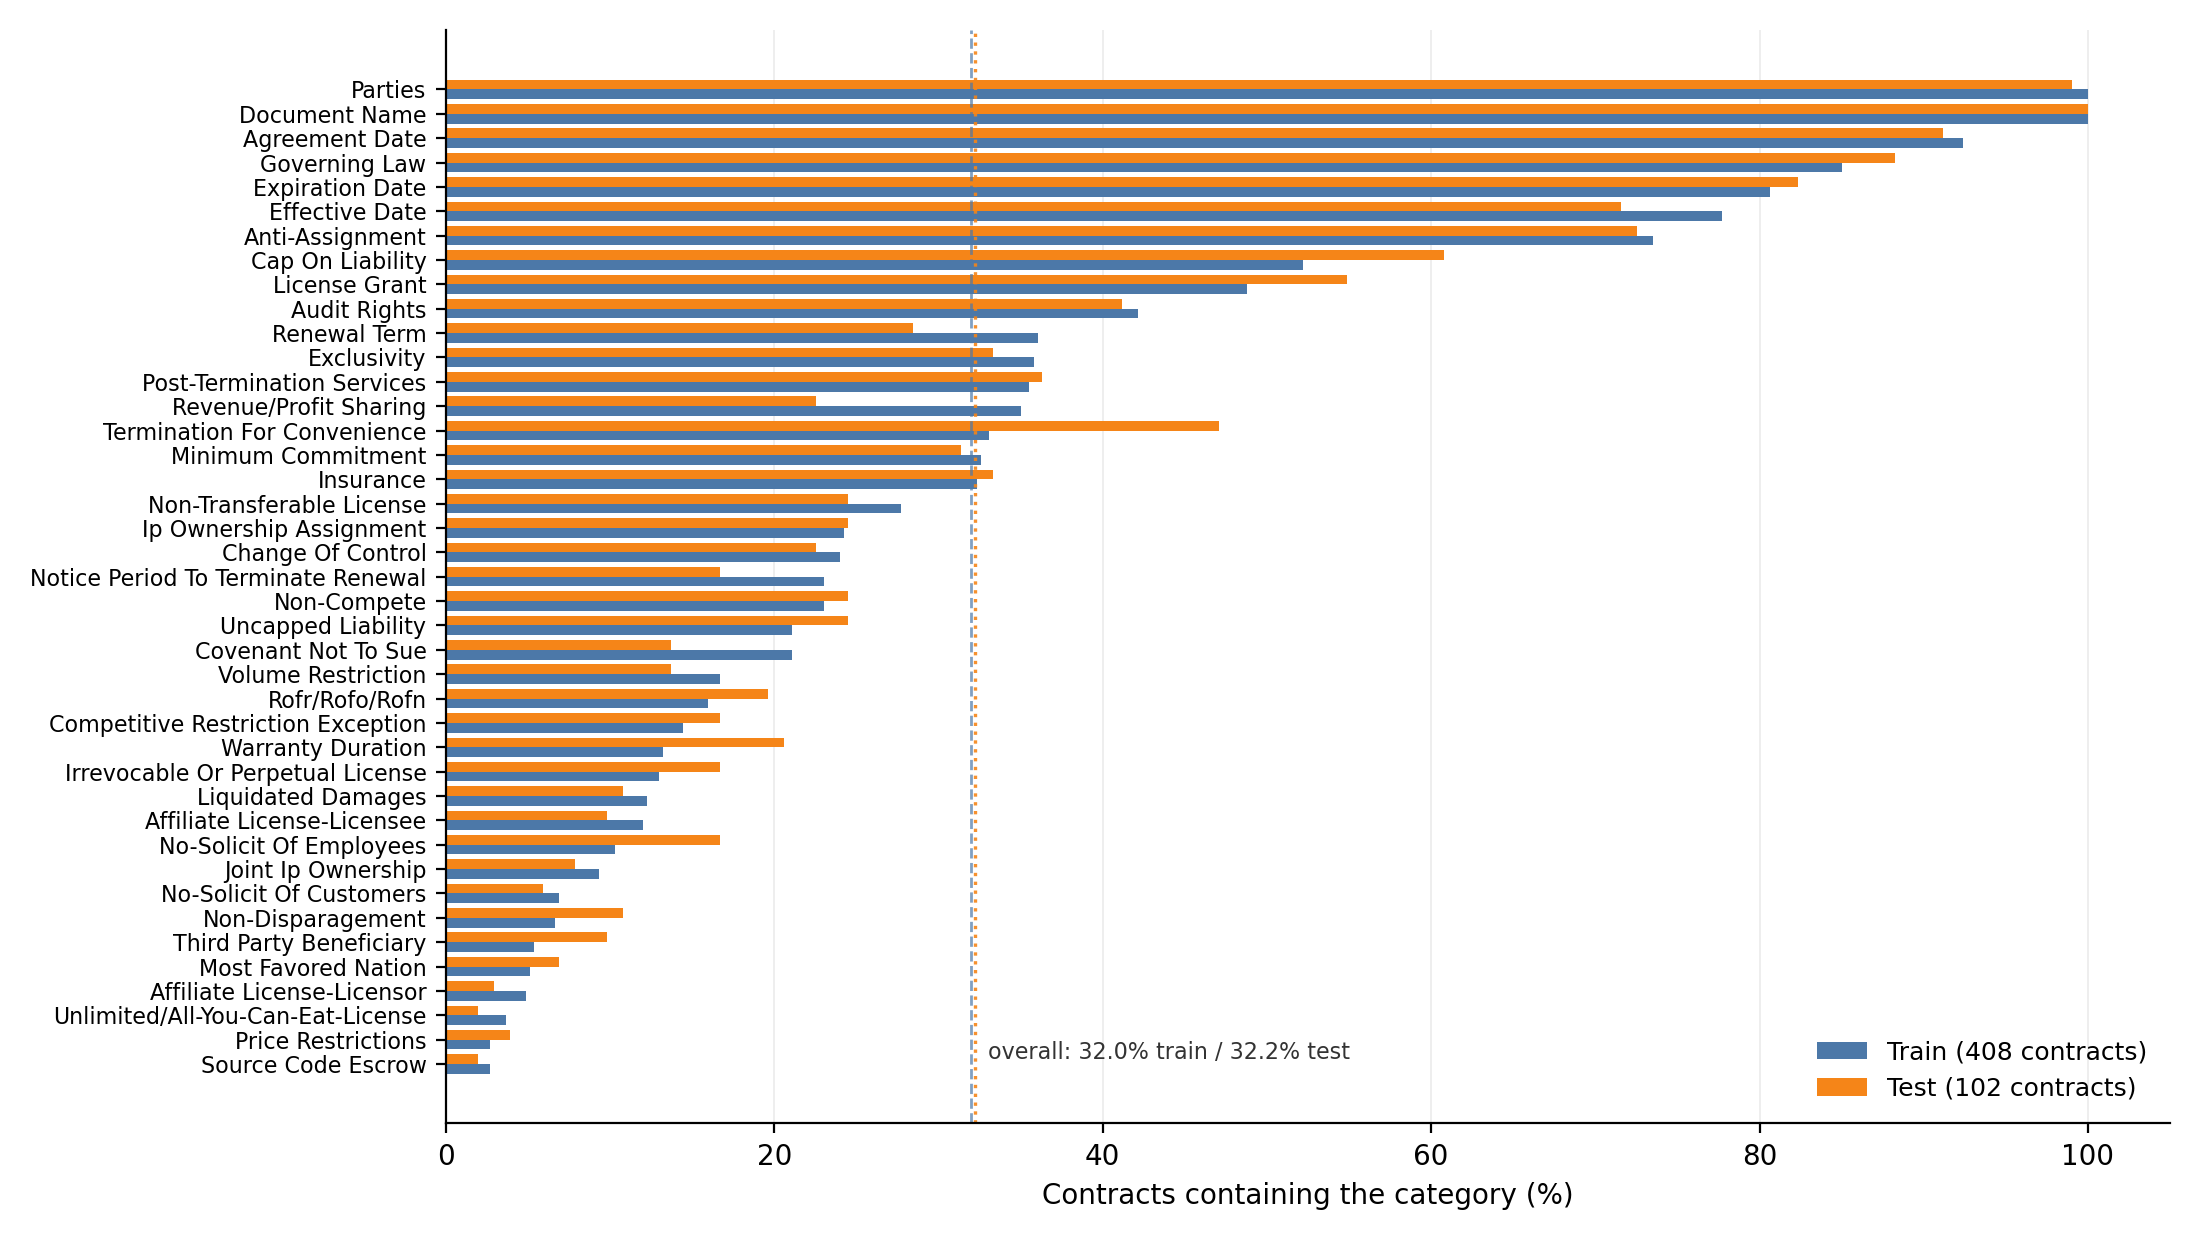
\includegraphics[width=\textwidth]{split_distribution.png}
\caption{Per-category split balance}
\label{fig:splitdist}
\end{figure}

\section{Implementation of Selected Design}
We built the chosen design in Python as two Jupyter notebooks, \texttt{train.ipynb} for preparing data and training and \texttt{test.ipynb} for testing on its own, plus some analysis scripts, and then turned it into the Clausify web app. This section describes how each model was trained and how the app works.

All models were trained only on the 408 training contracts (80\%). Training ran on one Apple-Silicon laptop with the MPS (Metal) backend, \texttt{torch} 2.8 and \texttt{transformers} 5.x. The summarizer ran on the CPU for the memory reasons explained in Section~\ref{sec:engineering}. Table~\ref{tab:hyper} lists the settings.

\begin{table}[ht]
\centering
\caption{Training configurations}
\label{tab:hyper}
\small
\begin{adjustbox}{max width=\textwidth}
\begin{tabular}{lccc}
\toprule
 & \textbf{Presence (MIL)} & \textbf{Span (QA)} & \textbf{Summarizer}\\
\midrule
Backbone            & DistilBERT-base & DistilBERT-base & FLAN-T5-small\\
Task head           & Sequence classification & QA (start/end) & Seq2seq LM\\
Training examples   & 24{,}000 (of 53{,}662) & 8{,}000 (of 11{,}156) & 4{,}000 (of 11{,}156)\\
Max input length    & 256 tokens (512 in the re-run) & 320 tokens & 256 in / 48 out\\
Epochs              & 2 & 2 & 2\\
Batch size          & 16 & 16 & 8\\
Learning rate       & $2\times10^{-5}$ & $3\times10^{-5}$ & $3\times10^{-4}$\\
Device              & MPS & MPS & CPU\\
Wall-clock          & $\approx$50--52 min & $\approx$23--26 min & $\approx$8--13 min\\
\bottomrule
\end{tabular}
\end{adjustbox}
\end{table}
\subsection{How We Validated, and Where the Settings Came From}
\label{sec:valprotocol}
If any setting in Table~\ref{tab:hyper} had been picked by trying several options and keeping the one that scored best on the 20\% test set, every number in Chapter~5 would be too optimistic and the test set would no longer be unseen. This section gives the source of each setting, including one place where we fell short.

\subsubsection{What was tuned, and what was not}
Nothing in Table~\ref{tab:hyper} was tuned. Every setting is a standard default for the model or a value fixed by reasoning before training, and no setting was ever compared with another on the test set. In detail:

\begin{itemize}[itemsep=3pt]
  \item The learning rates, batch sizes and epochs ($2\times10^{-5}$, $3\times10^{-5}$, $3\times10^{-4}$; 16/16/8; 2 epochs) are the standard fine-tuning defaults for DistilBERT and T5 models. We ran each setting once and did no search. This protects the test set, but it also means we only know these values are common, not that they are good.
  \item The window of 2{,}000 characters with a step of 1{,}500 comes from a measurement on the training data: the 500-character overlap must be longer than a typical clause (196 characters) so that no clause falls between windows (Section~\ref{sec:mil}). Any window and step that meet this rule would work, and we did not look for the best pair.
  \item Two negative windows per contract and category balance the classes, keeping about 39\% positives instead of letting almost all windows be negative. This was not tuned either.
  \item Taking the maximum window score was chosen because it is the multiple-instance rule. We did not try other rules at first; Section~\ref{sec:pooling} does so afterwards.
  \item The 0.5 threshold is the default boundary for a two-class model. Nobody chose, checked or changed it, and Section~\ref{sec:threshold} later shows that it is a poor choice for the window-based transformer.
\end{itemize}

This project avoided tuning on the test set by not tuning at all. That guarantees the test scores are fair, and it also limits them: the transformer may lose to the baseline partly because nobody looked for better settings for it. Section~\ref{sec:v2} confirms this. With the whole window read and both models tuned on a validation split, the gap closes.

\subsubsection{The validation sets actually used}
Table~\ref{tab:valsets} shows, for each model, what data was kept aside during training and what it was used for.

\begin{table}[ht]
\centering
\caption{Validation arrangements}
\label{tab:valsets}
\small
\begin{adjustbox}{max width=\textwidth}
\begin{tabular}{>{\raggedright\arraybackslash}p{2.6cm} >{\raggedright\arraybackslash}p{4.5cm} >{\raggedright\arraybackslash}p{6.2cm}}
\toprule
\textbf{Model} & \textbf{Validation data} & \textbf{Use}\\
\midrule
Presence (MIL) & 5\% of the \emph{training} windows, split off before training & Monitoring only. Clean: no test contract contributes.\\
\addlinespace
Span (QA) & None (\texttt{eval\_strategy="no"}) & No validation loss exists for this model.\\
\addlinespace
Summarizer (deployed checkpoint) & None & The checkpoint used in every reported result and in Clausify was trained with no evaluation set.\\
\bottomrule
\end{tabular}
\end{adjustbox}

{\footnotesize\singlespacing \emph{Note.} ``Monitoring only'' means the loss was printed and plotted but never used to select a checkpoint, stop early, or change a setting: all three runs used \texttt{save\_strategy="no"} and kept the final-step weights.\par}
\end{table}

\subsubsection{One thing we got wrong}
The first exploratory run of the summarizer in the notebook, whose loss curve appeared in earlier drafts of this report, monitored training on 300 clauses taken from the test split. That was the wrong data to monitor with, and we should not have done it.

Two facts limit the damage. That run kept no checkpoints (\texttt{save\_strategy="no"}) and had no early stopping, so the numbers it printed could not have been used to choose a model, and nothing about the model depended on them. The summarizer used for all results was also trained again by \texttt{build\_artifacts.py} with no evaluation set at all, and that model produced every summarizer result in Chapter~5. No reported score comes from a model chosen with test data.

The ``validation'' loss printed by that run (0.096 $\to$ 0.075) was really a loss on test clauses and should be ignored. The October 2026 re-training rebuilt the summarizer exactly as it is used, with no evaluation set, and Figure~\ref{fig:sumloss} now shows that run's training loss, so no test data appears in it. We kept this mistake in the report because it is easy to make: with a small dataset and three models, it is tempting to grab ``the other split'' when a validation set is needed. Writing down, for each model, exactly what was kept aside catches it, and Table~\ref{tab:valsets} now does that.
\subsection{Optimization Schedule}
Table~\ref{tab:hyper} gives the highest learning rate of each model, but the schedule that lowers it over time matters as much. All three models use the same optimizer setup: AdamW with a linear decay schedule, no warm-up, and gradient clipping at 1.0. Figure~\ref{fig:lrsched} plots the three schedules. We read the presence and span settings from the \texttt{training\_args.bin} file saved next to each model, so the plot shows what actually ran.

Two of these choices need a reason. Skipping warm-up is usually risky, but these are short fine-tuning runs (1{,}000--3{,}000 steps) that start from pre-trained weights with small learning rates. Warm-up mainly keeps the first updates of a randomly started model stable, which hardly applies here, and the smooth loss curves in Figures~\ref{fig:presloss} and~\ref{fig:sumloss} show no early problems. Gradient clipping at 1.0 stayed on throughout. Clipping is important on the MPS backend, because it stops a single bad batch from causing the kind of breakdown we saw with DeBERTa-v3 (Section~\ref{sec:engineering}).

\begin{figure}[ht]
\centering
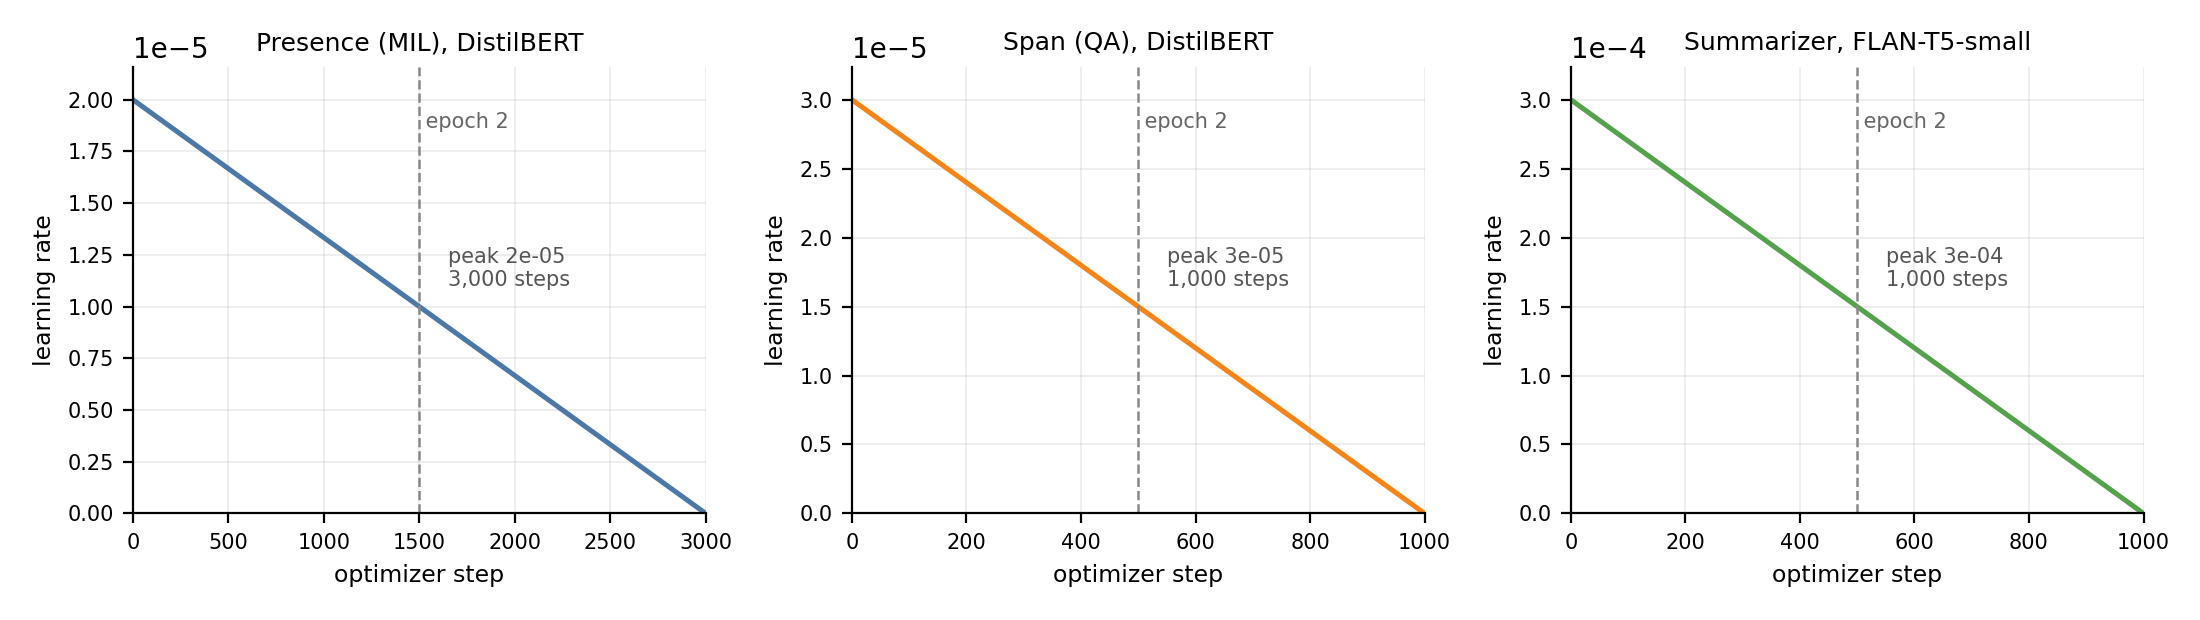
\includegraphics[width=\textwidth]{lr_schedule.png}
\caption{Learning-rate schedules}
\label{fig:lrsched}
\end{figure}

A record of the gradient size during training shows directly whether training stayed healthy, instead of leaving us to infer it from the loss. The original August runs did not keep it, because their temporary checkpoint folders were deleted after training. The October 2026 re-training logged it every 100 steps for all three models, and so did the August full-data presence run in Section~\ref{sec:budget}.

These logs show something the loss curves do not. In the October runs the gradient size ranges from 1.45 to 10.60 (median 4.30) for the presence model and from 10.11 to 20.92 (median 12.72) for the span model, so every logged step of both runs is above the clipping limit of 1.0. The August full-data presence run looks the same: across its 63 logged points the gradient size ranges from 0.55 to 11.96 with a median of 4.65, and 98.4\% of the points are above 1.0. The summarizer's gradients are much smaller (0.55 to 1.38, median 1.07, with 70\% of points above 1.0). Nothing broke in any run: there are no NaN values or large spikes, and the losses fall smoothly. For the two DistilBERT models, however, clipping was active on almost every step, so the update size was cut back all the time and the learning rates in Table~\ref{tab:hyper} overstate the real step size. This weakens the warm-up argument above a little, since part of what kept the early updates stable was almost certainly the clipping as well as the small learning rate. Our smooth loss curves are not good evidence that skipping warm-up is safe in general.
\subsection{Training the Presence Classifier}
\label{sec:prestrain}
The TF--IDF + logistic-regression baseline trains in under a minute. On the 20\% test set it reaches micro-F1 0.775, weighted-F1 0.777, macro-F1 0.572 over all 41 categories, and 0.666 over the 34 categories with at least ten test positives. The gap between micro and macro scores comes from the rare categories with very few examples.

The window-level DistilBERT was trained on a balanced sample of 24{,}000 window examples (39.2\% positives) to keep training manageable on a laptop. In the October 2026 re-training it took 49.8 minutes. The training loss fell smoothly from 0.57 after the first 100 steps to 0.26 at the end, and the validation loss went from 0.275 after the first epoch to 0.254 after the second (Figure~\ref{fig:presloss}). The validation loss stayed close to the training loss, so we saw no sign of over-fitting.

\begin{figure}[ht]
\centering
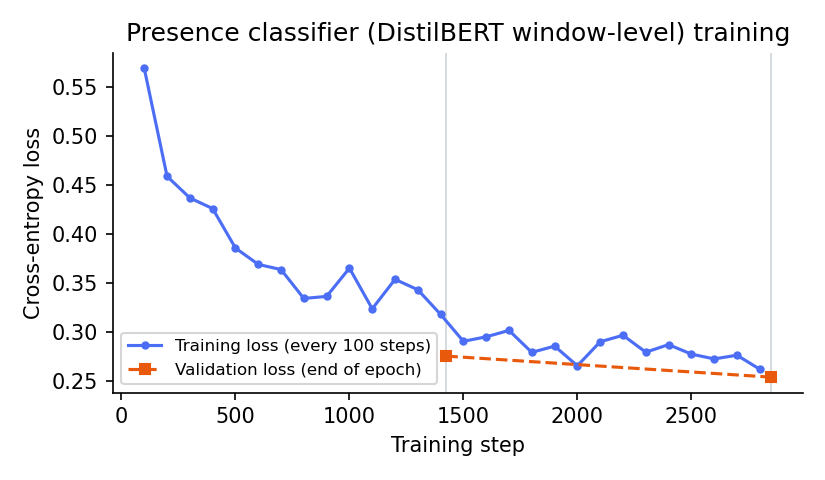
\includegraphics[width=0.62\textwidth]{presence_loss.png}
\caption{Presence classifier loss}
\label{fig:presloss}
\end{figure}
\subsection{Training the Span Extractor}
The question-answering model was trained on 8{,}000 focus-window examples for two epochs. Before training, we turn the labelled token positions back into text for a few examples and check that they match the marked answers. In SQuAD-style systems the character-to-token conversion is easy to get wrong without noticing, and this small check catches that.
\subsection{Training the Summarizer}
\label{sec:sumtrain}
FLAN-T5-small was fine-tuned on 4{,}000 clause--template pairs on the CPU. This took about 8 minutes originally and 12.7 minutes in the October 2026 re-training, which ran while the laptop was busy with other jobs. The training loss dropped quickly, from 1.17 at step 100 to 0.08 by the end of the second epoch (Figure~\ref{fig:sumloss}). There is no validation curve because the model used in the app is trained with no evaluation set (Table~\ref{tab:valsets}). The re-trained model scores ROUGE-L 0.775 against the templates on the 150 test clauses, the same as the original. In hindsight, the fast drop was the first sign of the template copying we analyze in Chapter~5: with only 41 different targets, the task is easy to learn.

\begin{figure}[ht]
\centering
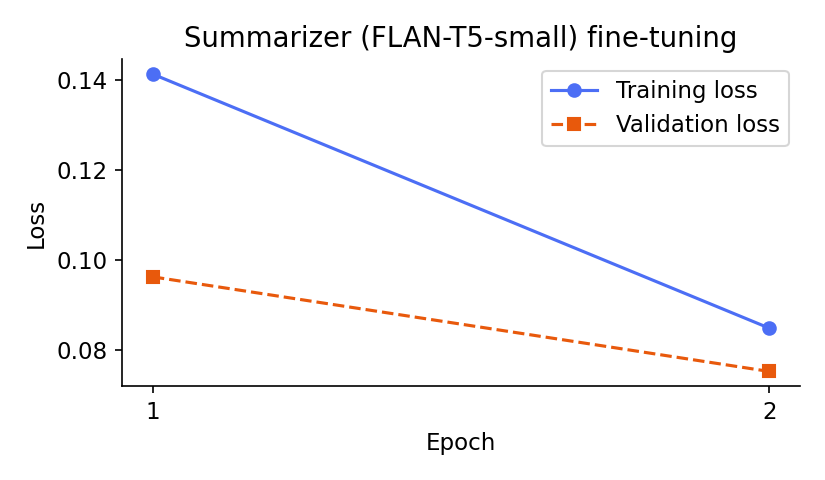
\includegraphics[width=0.62\textwidth]{summarizer_loss.png}
\caption{Summarizer loss}
\label{fig:sumloss}
\end{figure}
\subsection{Engineering Notes: Training on Consumer Hardware}
\label{sec:engineering}
A few practical lessons may save time for anyone repeating this work on Apple-Silicon computers:
\begin{itemize}[itemsep=2pt]
  \item DeBERTa-v3 is unstable on MPS. Our first-choice model produced NaN (broken) gradients on the MPS backend and was far too slow on the CPU (about 89 seconds per step). We switched to DistilBERT; the method stays the same, and on a CUDA machine the model name can simply be changed back.
  \item MPS memory is not freed inside one program. After two transformer trainings in the same session, the summarizer ran out of MPS memory even after we deleted objects and cleared the cache. What actually works is restarting the kernel or training the (small) summarizer on the CPU, which is what we did.
  \item Library changes. \texttt{transformers} 5.x renamed \texttt{Trainer(tokenizer=\dots)} to \texttt{processing\_class=\dots}. We also turned off mixed precision (\texttt{fp16=bf16=False}) and converted the loss logits to fp32 to avoid data-type problems on MPS.
  \item Repeatability. Everything needed (the split in \texttt{artifacts/split.json}, the baseline in \texttt{artifacts/baseline.pkl}, and the three trained models) is saved to disk, and a separate test notebook recreates every number in Chapter~5 from those files alone.
\end{itemize}
\subsection{Measured: What Sparse Attention Would Have Cost}
\label{sec:lfbench}
Section~\ref{sec:lit_long} argued against sparse attention partly because of cost, and a cost argument is weak until the cost is measured. The laptop used for this project is exactly the machine in question, so we measured it.

We built Longformer-base at its published size (12 layers, 768 hidden units, 4{,}098 position embeddings, attention window 512, 148.7M parameters). We timed one forward pass at 4{,}096 tokens and one full training step (forward pass, backward pass and AdamW update), and compared them with the DistilBERT setup this project used. The weights are random, which does not matter here, because time and memory depend on the size of the tensors and not on their values. Each setup ran in its own program, so the peak memory belongs to that setup alone. The machine is an Apple M4 with 16\,GB of shared memory, which the operating system also uses. Table~\ref{tab:lfbench} shows the results.

\begin{table}[ht]
\centering
\caption{Longformer vs.\ DistilBERT cost}
\label{tab:lfbench}
\small
\begin{adjustbox}{max width=\textwidth}
\begin{tabular}{llccc}
\toprule
\textbf{Model} & \textbf{Operation} & \textbf{Batch} & \textbf{Time} & \textbf{Peak memory}\\
\midrule
Longformer-base (148.7M) & forward, 4{,}096 tok & 1 & 3.69\,s & 2.18\,GB\\
DistilBERT (67.0M)       & forward, 256 tok     & 16 & 0.19\,s & 1.15\,GB\\
\addlinespace
Longformer-base & training step, 4{,}096 tok & 1 & 258\,s & 14.71\,GB\\
Longformer-base & training step, 4{,}096 tok & 2 & 2{,}170\,s & 20.75\,GB\\
DistilBERT      & training step, 256 tok     & 16 & 3.17\,s & 4.47\,GB\\
\bottomrule
\end{tabular}
\end{adjustbox}

{\footnotesize\singlespacing \emph{Note.} Measured on the Apple M4 (16\,GB unified memory) that trained every model reported in this project.\par}
\end{table}

This measurement corrected us. Before measuring, we believed that fine-tuning a Longformer at 4{,}096 tokens was not possible on one laptop (Section~\ref{sec:lit_long}). At batch size 1 it fits, using 14.71\,GB on a 16\,GB machine. That leaves less than 1.5\,GB for the operating system, but the model, its gradients and its optimizer state all fit in memory and the step finishes.

One step further, the memory claim holds. At batch size 2 the memory needed rises to 20.75\,GB, more than the machine has, and the timing shows it: the step takes 2{,}170 seconds instead of the roughly 516 that doubling the batch should take. Being 8.4 times slower for twice the work means the computer is swapping memory to disk. The accurate claim is that Longformer fits only at batch size 1, and any batch size a real training run would use does not fit.

Time is the real limit. At 258 seconds per step and batch size 1, repeating our two-epoch presence training (22{,}800 training windows, 45{,}600 examples seen in total) would take about 136 days of non-stop computing. The DistilBERT run it would replace took about 50 minutes. Short tests add start-up time (our own DistilBERT step takes 3.17\,s here but about 1.0\,s during the real run), so these numbers may be about three times too high. Even then, a third of 136 days is still 45 days, and the project had weeks.

Measurement also confirms the cost when the app runs. Scanning one typical contract (33{,}143 characters) for all 41 categories takes 22 windows $\times$ 41 $\times$ 11.7\,ms $\approx$ 10.6 seconds with our DistilBERT, against 3 windows $\times$ 41 $\times$ 3.69\,s $\approx$ 454 seconds (seven and a half minutes) with Longformer. Clausify is meant to respond within seconds, so this rules Longformer out for the app, whatever a large training computer could do.

None of this shows that a Longformer would have scored worse. It shows only that we could not have found out on this hardware, a much narrower claim than the one we started with. Settling the modelling question needs a CUDA machine, and we list it as future work.
\subsection{End-to-End Data Flow}
Figure~\ref{fig:pipeline} names the steps, and Figure~\ref{fig:dataflow} adds what passes between them. The sizes shown are for one contract of typical length.

\begin{figure}[ht]
\centering
\begin{adjustbox}{max width=\textwidth}
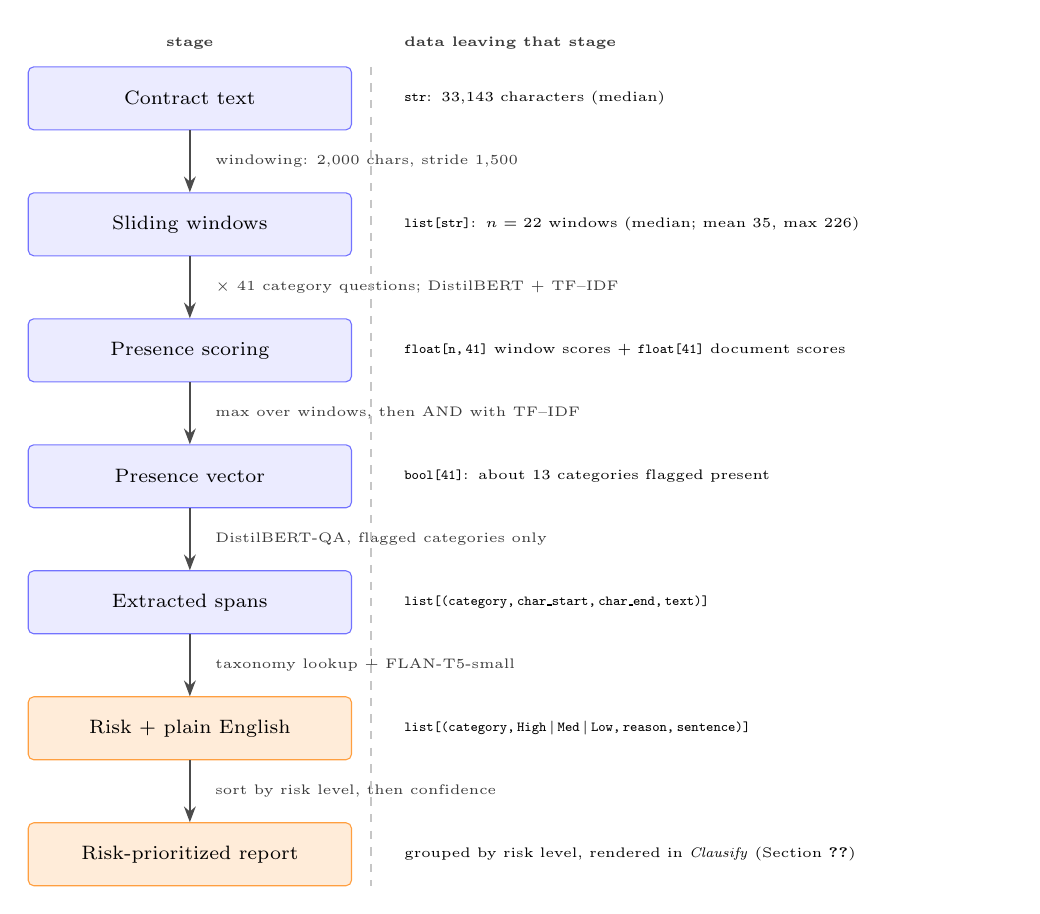
\begin{tikzpicture}[x=1mm, y=1mm, font=\scriptsize,
  st/.style={draw=blue!55, fill=blue!8, rounded corners=2pt, text width=40mm,
             align=center, minimum height=8mm, inner sep=1.5pt},
  ad/.style={st, draw=orange!75, fill=orange!15},
  arr/.style={-{Stealth[length=2mm]}, gray!60!black, line width=0.6pt},
  op/.style={font=\tiny, text=gray!45!black, anchor=west},
  dat/.style={font=\tiny, anchor=west, text width=76mm}
]
\node[st] (s1) at (24,0)   {Contract text};
\node[st] (s2) at (24,-16) {Sliding windows};
\node[st] (s3) at (24,-32) {Presence scoring};
\node[st] (s4) at (24,-48) {Presence vector};
\node[st] (s5) at (24,-64) {Extracted spans};
\node[ad] (s6) at (24,-80) {Risk $+$ plain English};
\node[ad] (s7) at (24,-96) {Risk-prioritized report};

\foreach \a/\b in {s1/s2, s2/s3, s3/s4, s4/s5, s5/s6, s6/s7} \draw[arr] (\a) -- (\b);

\node[op] at (26,-8)  {windowing: 2{,}000 chars, stride 1{,}500};
\node[op] at (26,-24) {$\times$ 41 category questions; DistilBERT $+$ TF--IDF};
\node[op] at (26,-40) {$\max$ over windows, then AND with TF--IDF};
\node[op] at (26,-56) {DistilBERT-QA, flagged categories only};
\node[op] at (26,-72) {taxonomy lookup $+$ FLAN-T5-small};
\node[op] at (26,-88) {sort by risk level, then confidence};

\node[dat] at (50,0)   {\texttt{str}: 33{,}143 characters (median)};
\node[dat] at (50,-16) {\texttt{list[str]}: $n = 22$ windows (median; mean 35, max 226)};
\node[dat] at (50,-32) {\texttt{float[n,\,41]} window scores $+$ \texttt{float[41]} document scores};
\node[dat] at (50,-48) {\texttt{bool[41]}: about 13 categories flagged present};
\node[dat] at (50,-64) {\texttt{list[(category,\,char\_start,\,char\_end,\,text)]}};
\node[dat] at (50,-80) {\texttt{list[(category,\,High\,$|$\,Med\,$|$\,Low,\,reason,\,sentence)]}};
\node[dat] at (50,-96) {grouped by risk level, rendered in \emph{Clausify} (Section~\ref{sec:clausify})};

\draw[gray!45, dashed, line width=0.4pt] (47,4) -- (47,-100);
\node[anchor=south, font=\tiny, text=gray!45!black] at (24,5) {\textbf{stage}};
\node[anchor=south west, font=\tiny, text=gray!45!black] at (50,5) {\textbf{data leaving that stage}};
\end{tikzpicture}
\end{adjustbox}
\caption{Pipeline data flow}
\label{fig:dataflow}
\end{figure}
\subsection{The Clausify Application}
\label{sec:clausify}
\subsubsection{Purpose and Design}
The final result of the project is \emph{Clausify}, a Streamlit web app that runs all of the project's trained models on any contract the user gives it (the re-run DistilBERT presence model and its TF--IDF partner from Section~\ref{sec:v2}, the span model, the FLAN-T5 summarizer, and the first setup's presence model for clause mode) and shows the results as a report sorted by risk. It is the system of Figure~\ref{fig:pipeline} with an interface. The design goal is that a non-lawyer should see the ``watch out before signing'' items first. Clauses found are grouped \textcolor{riskhigh}{\textbf{High}} $\rightarrow$ \textcolor{riskmed}{\textbf{Medium}} $\rightarrow$ \textcolor{risklow}{\textbf{Low}} and sorted by model score within each group.
\subsubsection{User Workflow}
\begin{enumerate}[itemsep=2pt]
  \item Add a contract. The user pastes the text or uploads a \texttt{.pdf}, \texttt{.docx} or \texttt{.txt} file, and the text is read on the user's own computer (Figure~\ref{fig:apphome}). The user picks \emph{Whole contract}, \emph{Separate clauses} (Section~\ref{sec:clausemode}) or \emph{Auto}. A settings panel chooses the detection rule and turns the plain-English lines on or off. The rules are the three re-run setups of Section~\ref{sec:v2}, with the thresholds chosen there: the recall-first transformer (the default), the recall-first ensemble and the balanced AND-ensemble.
  \item Analyze. One click runs all the models, and a progress bar follows the scan of the 41 categories and then the summarizer.
  \item Read the report. A summary bar counts the clauses found at each risk level (Figure~\ref{fig:appresults}), and each clause appears below it as a card. On the made-up test contract the bar shows 5 High, 13 Medium and 9 Low risk clauses, so 27 of the 41 categories are found (re-run model, recall-first default).
\end{enumerate}

\begin{figure}[ht]
\centering
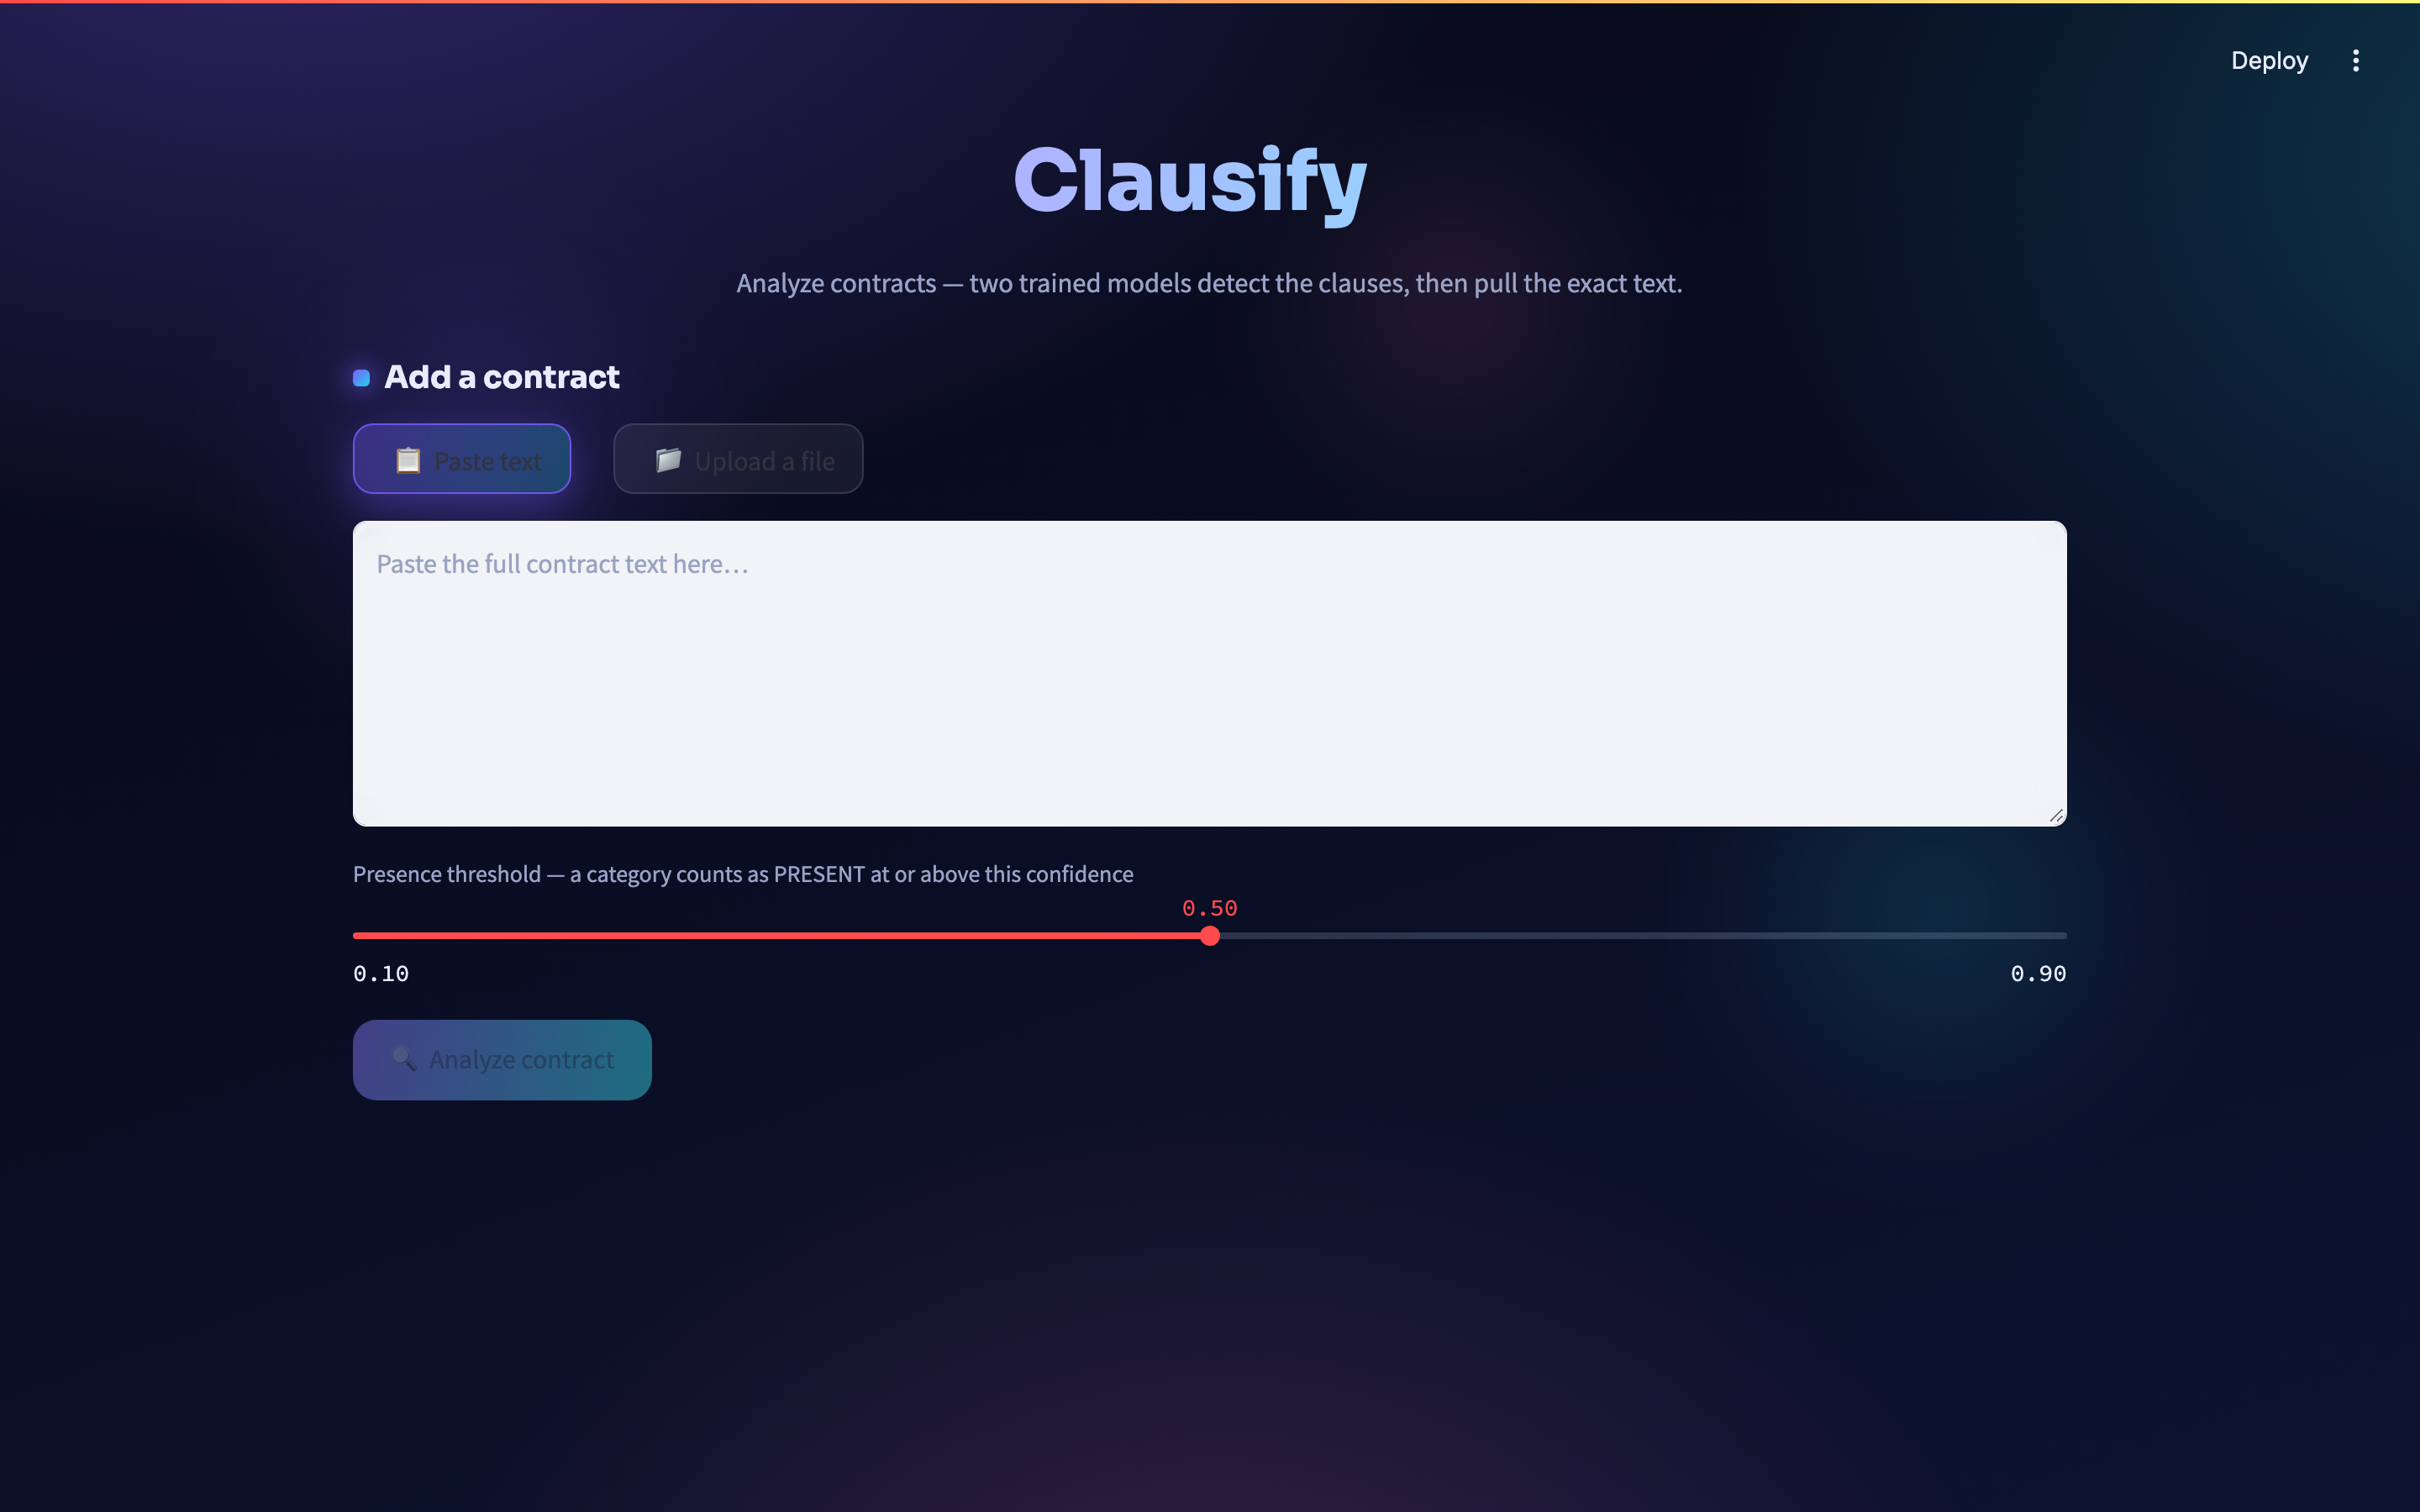
\includegraphics[width=0.95\textwidth]{app_home.png}
\caption{Clausify input screen}
\label{fig:apphome}
\end{figure}

Each clause card shows the category name with a coloured risk badge, the one-line reason why that category is risky (from the risk table in Appendix~\ref{app:taxonomy}), the summarizer's plain-English sentence with a warning when it belongs to another category, the detection score as a bar with both the DistilBERT and TF--IDF scores, and the clause quoted from the user's own contract with the span model's key phrase highlighted (Figure~\ref{fig:appcards}). Below the cards the app adds three more views:
\begin{itemize}[itemsep=2pt]
  \item A highlighted contract: the full text, with every clause found marked in its risk colour and labelled with its category. Each card links to its place in the text.
  \item A missing-protection checklist: protective clauses the models did not find, namely a limit on liability, termination for convenience, governing law, an expiry date, a warranty period, insurance and, when the contract renews itself, a notice period to stop the renewal. Each comes with a sentence on why its absence matters, and the view notes that ``not detected'' can also mean the model missed it.
  \item A downloadable report: a PDF (summary, every clause with its reason, plain-English line, scores and quoted text, and the checklist) and a CSV file with the same rows.
\end{itemize}

\begin{figure}[ht]
\centering
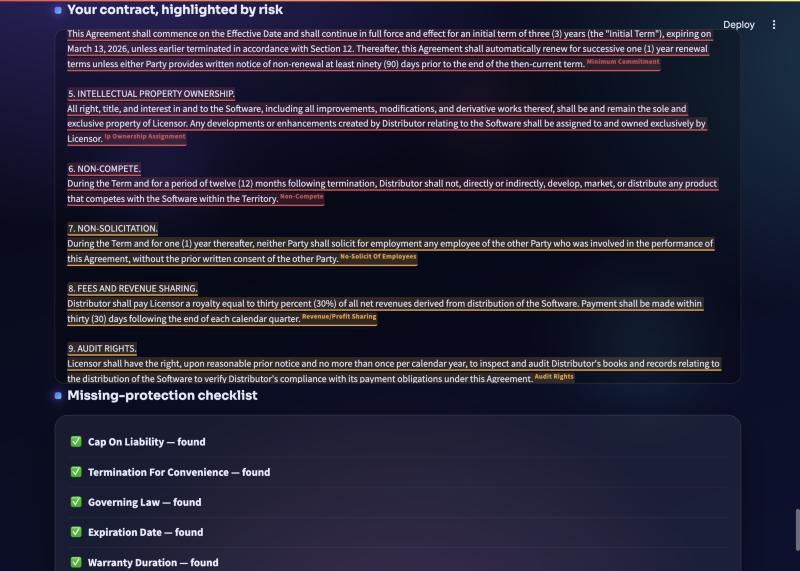
\includegraphics[width=0.95\textwidth]{app_highlight.png}
\caption{Highlighted contract and checklist}
\label{fig:apphighlight}
\end{figure}

Figure~\ref{fig:apphighlight} shows the highlighted view and the checklist on the made-up test contract. The renewal paragraph is labelled \emph{Renewal Term}; the first setup's model labelled it \emph{Minimum Commitment}, which was wrong. The checklist reports the warranty period as not detected although Section~10 of the contract sets one (90 days), and Figure~\ref{fig:appresults} shows a false alarm: the liability clause, which caps liability, is reported as \emph{Uncapped Liability}. The summarizer's warning on that card points to the right category. We kept both mistakes in the figures instead of choosing cleaner examples.

\begin{figure}[ht]
\centering
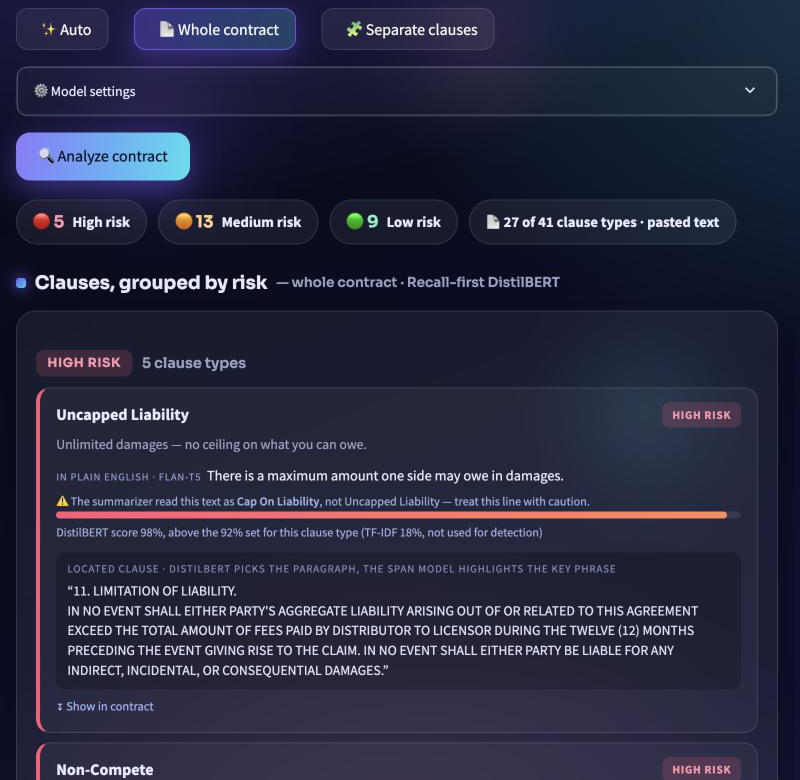
\includegraphics[width=0.95\textwidth]{app_results.png}
\caption{Clausify results view}
\label{fig:appresults}
\end{figure}

\begin{figure}[ht]
\centering
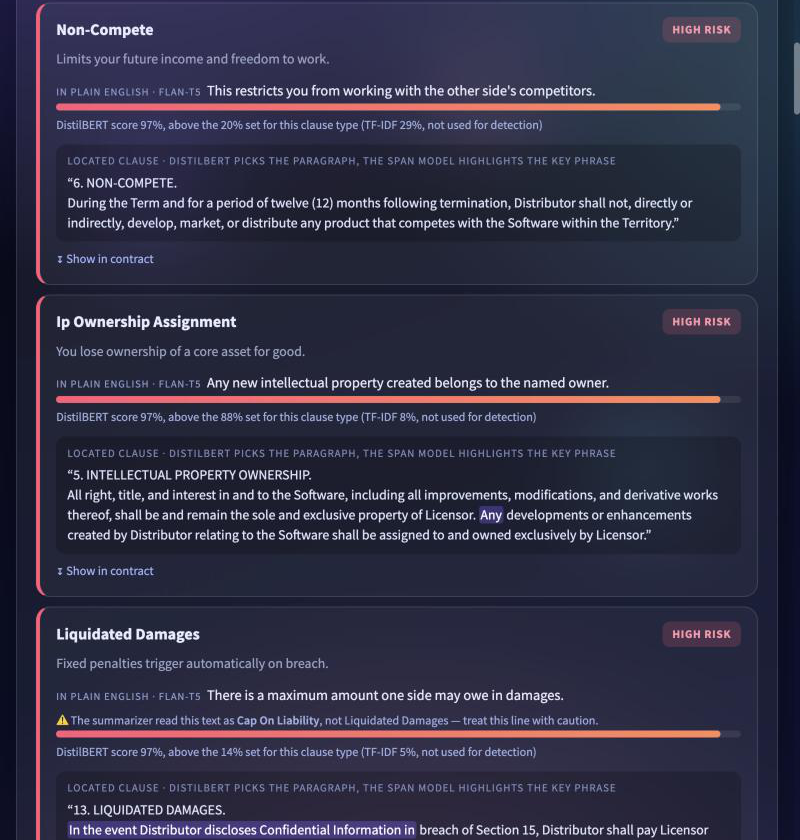
\includegraphics[width=0.95\textwidth]{app_cards.png}
\caption{High-risk clause cards}
\label{fig:appcards}
\end{figure}
\subsubsection{How the Models Run Inside the App}
The app follows the same steps that were used in testing:
\begin{enumerate}[itemsep=2pt]
  \item Windows. The contract is cut into 2{,}000-character windows that move forward 1{,}500 characters at a time, as in training. At most 30 windows are read, so very long documents stay fast.
  \item Model 1, presence. For each of the 41 categories, the exact CUAD question the model was trained on is paired with every window and scored by the re-run DistilBERT, which reads the whole window (512 tokens). The score for the whole contract is the highest window score. A category is reported as present when its score reaches the threshold chosen for it on the validation split, and the best window is remembered.
  \item Finding the clause. Inside that best window, the presence model scores each paragraph against the category question, and the highest-scoring paragraph is quoted on the card. The DistilBERT question-answering model then highlights the key phrase inside it. An earlier version let the span model choose the text from the whole window, and on test inputs it returned the same sentence for almost every category, because the span model prefers text near the position where answers sat during training (Section~\ref{sec:e2e}). It is now used only inside the paragraph the presence model chose.
  \item Optional ensembles. With these settings the re-run TF--IDF model also scores the whole contract. The recall-first ensemble reports a category when the average of the two scores reaches that category's threshold, and the balanced ensemble when both scores reach their own thresholds, exactly as tested in Section~\ref{sec:v2}. The thresholds are stored in \texttt{decision\_v2.json}, which the training code writes and the app reads, so the app cannot drift from the tested setup.
  \item Risk layer. The category found is looked up in the fixed risk table (8 High, 22 Medium, 11 Low) for its level and reason.
  \item Summarizer. FLAN-T5-small receives each quoted clause with the same prompt and settings as in testing and returns one plain-English sentence.
\end{enumerate}

All the models run on the CPU, so the app works on any computer, and a typical contract takes about a minute once the models are loaded (Table~\ref{tab:appbench}). The app loads the trained models saved by the training code (\texttt{presence\_mil}, \texttt{span}, \texttt{summarizer} and the TF--IDF \texttt{baseline.pkl}). When they are not on the computer, as on a cloud server, it downloads the same files once from a public Hugging Face model repository.
\subsubsection{Implementation Notes}
The app is a single-page Streamlit program (\texttt{app.py}) built on two small modules. \texttt{model\_utils.py} loads the models and handles windows, scoring, clause finding, the summarizer and the risk table, and \texttt{features.py} reads uploaded files, builds the highlighted view and creates the reports. Two test contracts come with the app: a real CUAD contract, and a made-up ``Master Software License and Distribution Agreement'' that we wrote to cover many of the 41 categories. On the made-up contract the app finds clauses at all three risk levels and puts the four High-risk clause types that the contract's section headings name (\emph{Exclusivity}, \emph{IP Ownership Assignment}, \emph{Non-Compete} and \emph{Liquidated Damages}) at the top of the report, which are the before-you-sign warnings the design aims for. It also reports one High-risk type the contract does not contain (Section~\ref{sec:v2}).
\subsubsection{Clause-by-Clause Mode}
\label{sec:clausemode}
Users often paste a few clauses instead of a whole contract and expect one card per clause. Whole-contract mode does not work that way. For each of the 41 categories it asks whether the category appears anywhere in the window, so six related clauses pasted together gave fourteen categories, eight of them wrong. The app therefore has a second mode, chosen automatically for a short list of paragraphs or chosen by the user, in which each paragraph is one clause and gets exactly one category and one risk level. When most paragraphs are numbered (``1.'', ``4.2'', ``(a)'', ``Section 5''), only the numbered ones are treated as clauses. The title, opening paragraph and signature lines are listed separately as skipped, so a contract with 18 numbered clauses gives exactly 18 cards, numbered as in the contract.

In this mode, if a clause heading names a category (``\textsc{2. Exclusivity.}''), the heading decides the category directly, and headings that do not clearly name one category are ignored. Otherwise the presence model scores the clause against all 41 category questions. Clause mode keeps the first setup's presence model, because the adjustment below and the accuracy figures reported for it were measured with that model. The raw scores cannot be compared across categories as they are; \emph{Parties}, for example, scores about 0.98 on almost any clause that names the two sides. Each category's score is therefore adjusted by how that category scores on real CUAD clauses of other categories, using 1{,}586 clauses from the training split, and the clause gets the category with the highest adjusted score. A clause whose best adjusted score is below 2 is shown as \emph{unrecognized} instead of being forced into a category.

On 721 clauses from the test split, this adjustment raises the share of clauses given the right category out of 41 from 9.6\% (raw highest score) to 42.3\%. The right category is in the top three 65.3\% of the time, and the right risk level is given 67.0\% of the time. These scores are well below the whole-contract ones, which we expected, since the presence model was trained to scan 2{,}000-character windows and not to label single clauses. The app shows these numbers under every clause-mode result. On the six-clause example above, the version with headings is labelled correctly (five High, one Low). With the headings removed, the model alone gets none of the six risk levels right: it labels five of them Medium and leaves one unrecognized. For inputs like this the clause headings provide the accuracy, and cards decided by the model alone should be checked against the clause text.

\subsubsection{Measured Latency}
\label{sec:appbench}
Chapter~2 explained that we chose a small model partly because the app must respond quickly. Section~\ref{sec:lfbench} measured what the alternative would have cost. Here we measure how fast our app is, running the app's own code on test contracts of different lengths.

\begin{table}[ht]
\centering
\caption{Application latency}
\label{tab:appbench}
\small
\begin{adjustbox}{max width=\textwidth}
\begin{tabular}{lrrrrr}
\toprule
 & & & \multicolumn{2}{c}{\textbf{Time}} & \\
\cmidrule(lr){4-5}
\textbf{Contract} & \textbf{Characters} & \textbf{Windows scored} & \textbf{First setup} & \textbf{Current app} & \textbf{Peak RSS}\\
\midrule
Shortest in test set & 1{,}283 & 1 & 2.7\,s & 3.1\,s & 1.25\,GB\\
25th percentile & 18{,}104 & 12 & 15.0\,s & 30.4\,s & 1.72\,GB\\
Median & 35{,}136 & 24 & 30.1\,s & 58.7\,s & 1.97\,GB\\
75th percentile & 65{,}547 & 30 (capped) & 32.7\,s & 96.6\,s & 2.07\,GB\\
Longest in test set & 289{,}615 & 30 (capped) & 34.8\,s & 102.8\,s & 2.13\,GB\\
\midrule
\multicolumn{6}{l}{\emph{Current app: median 58.7\,s \quad mean 58.3\,s \quad worst case 102.8\,s}}\\
\bottomrule
\end{tabular}
\end{adjustbox}

{\footnotesize\singlespacing \emph{Note.} Measured in October 2026 through the application's own \texttt{analyze()} entry point with its default detection rule, on the same machine with nothing else running. First setup: the 256-token presence model. Current app: the re-run 512-token model of Section~\ref{sec:v2}. CPU only, Apple M4, models already loaded (loading adds 0.6\,s). Peak RSS is the memory of the whole Python process for the current app.\par}
\end{table}

A typical contract takes about a minute (58.7 seconds for the median test contract). That is about twice the first setup's 30.1 seconds, because the presence model now reads twice as much text in every window. It is the price of the accuracy gain in Section~\ref{sec:v2}. Our first guess of 5--15 seconds came from watching the demo on short inputs.

Two design effects show in the numbers. Time grows in proportion to the number of windows, because most of the work is 41 categories $\times$ windows passes through DistilBERT, with each (category, window) pair scored once and nothing reused between categories. The 30-window limit keeps the worst case short. Without it the longest test contract would take more than ten minutes, but with it every contract longer than about 45{,}500 characters is cut at the same point. The limit buys speed with a hidden cost in recall: clauses after the cut cannot be found, and no Chapter~5 number shows this, because those tests read the full document. It is a limit of the app and not of the method, and Section~\ref{sec:demolimits} says so.



\chapter{Result Analysis}
\section{Performance Evaluation}
\textbf{What we measure.} Each step is measured with the score that fits its task. \emph{Finding which clauses are present} is a yes/no decision for each of the 4{,}182 (contract, category) test pairs. We score it with micro-F1 (every decision counts the same), macro-F1 (every category counts the same), and the accuracy, precision, recall and specificity from the confusion matrix. \emph{Finding the clause text} is scored with token-level F1, exact match, and the share of answers that overlap the real clause with F1~$\geq$~0.5. \emph{Summarizing} is scored with ROUGE-L against two different sets of reference sentences. The \emph{whole system} is scored by the share of real clauses that get through every step, and the risk layer by how many clauses it finds at each risk level. Speed is measured as the time and memory the app needs (Table~\ref{tab:appbench}).

\textbf{How we test.} Every model is tested once on the same 102 test contracts, using a separate notebook that loads the saved models from disk. Uncertainty is measured with a bootstrap over contracts, and we check whether the main result changes with the amount of training data, the random seed, the way window scores are combined, the decision threshold and the train/test split.

Everything in this chapter is measured on the 20\% test set: the same 102 unseen contracts for every model. All numbers come from the October 2026 re-training (Chapter~4) unless a run is marked as from August 2026. They were produced by a separate test notebook that loads the trained models from disk, so nothing left over from training can affect them.
\subsection{Presence Classification}
\subsubsection{Model comparison}
Table~\ref{tab:ensemble} and Figure~\ref{fig:ensemble} compare all the presence models on the 4{,}182 (contract, category) test decisions. Two things stand out. First, the window-based transformer \emph{loses on its own} to the simple TF--IDF model that reads the whole document (0.692 vs.\ 0.775). Legal wording is distinctive enough that word evidence from the whole document beats meaning-based evidence from small windows, and taking the maximum window score creates too many false alarms, just as Section~\ref{sec:mil} predicted. Second, the AND-ensemble, which reports a clause only when \emph{both} models agree, removes many of each model's false alarms and comes out on top (0.779). The lead over the simple model is small on 102 test contracts, so we do not rely on it: Section~\ref{sec:bootstrap} measures exactly how small it is and finds that this gap cannot be told apart from zero. The conclusion we stand behind is about method: \emph{simple word-based models are strong at deciding which clauses a contract contains, and the transformer is useful as a filter that removes false alarms, not as a replacement}.

\begin{table}[!htbp]
\centering
\caption{Presence model comparison}
\label{tab:ensemble}
\begin{adjustbox}{max width=\textwidth}
\begin{tabular}{lc}
\toprule
\textbf{Model} & \textbf{micro-F1}\\
\midrule
\textbf{Ensemble AND (both must agree)} & \textbf{0.779}\\
TF--IDF baseline (full document)        & 0.775\\
Ensemble AVG (mean probability)         & 0.718\\
Transformer (max-pool) alone            & 0.692\\
Ensemble OR (either fires)              & 0.692\\
\addlinespace
\multicolumn{2}{l}{\emph{August 2026 control run, Section~\ref{sec:budget}:}}\\
Transformer trained on all 53{,}662 windows & 0.694\\
Ensemble AND on that transformer            & 0.782\\
\bottomrule
\end{tabular}
\end{adjustbox}

{\footnotesize\singlespacing \emph{Note.} micro-F1 over all 4{,}182 test decisions. The transformer (0.6924) is just ahead of OR (0.6916).\par}
\end{table}

\begin{figure}[!htbp]
\centering
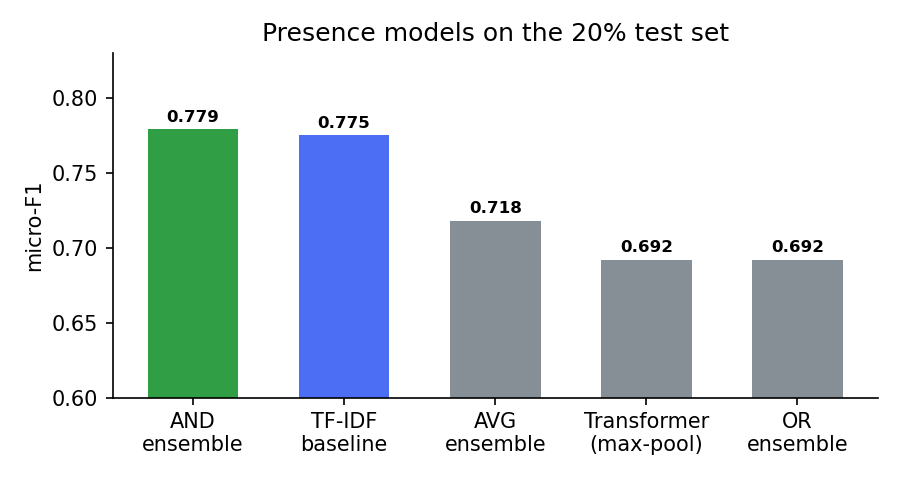
\includegraphics[width=0.75\textwidth]{ensemble_comparison.png}
\caption{Presence model micro-F1}
\label{fig:ensemble}
\end{figure}
\subsubsection{Confusion-matrix analysis}
Our test plan required a full confusion-matrix analysis of the final model. Table~\ref{tab:cm} gives the matrix for the AND-ensemble over all test decisions, Figure~\ref{fig:cm} shows the same matrix as a heatmap, and Table~\ref{tab:metrics} lists every score taken from it.

\begin{table}[!htbp]
\centering
\caption{AND-ensemble confusion matrix}
\label{tab:cm}
\begin{adjustbox}{max width=\textwidth}
\begin{tabular}{lcc}
\toprule
 & \textbf{Predicted Absent} & \textbf{Predicted Present}\\
\midrule
\textbf{Actually Absent}  & TN = 2{,}525 & FP = 309\\
\textbf{Actually Present} & FN = 291     & TP = 1{,}057\\
\bottomrule
\end{tabular}
\end{adjustbox}
\end{table}

\begin{table}[!htbp]
\centering
\caption{Confusion-matrix metrics}
\label{tab:metrics}
\begin{adjustbox}{max width=\textwidth}
\begin{tabular}{llc}
\toprule
\textbf{Metric} & \textbf{Formula} & \textbf{Value}\\
\midrule
Accuracy    & $(TP+TN)/\text{all}$          & 85.65\%\\
Precision   & $TP/(TP+FP)$                  & 77.38\%\\
Recall (Sensitivity) & $TP/(TP+FN)$         & 78.41\%\\
Specificity & $TN/(TN+FP)$                  & 89.10\%\\
F1 score    & $2PR/(P+R)$                   & 0.7789\\
\bottomrule
\end{tabular}
\end{adjustbox}
\end{table}

\begin{figure}[!htbp]
\centering
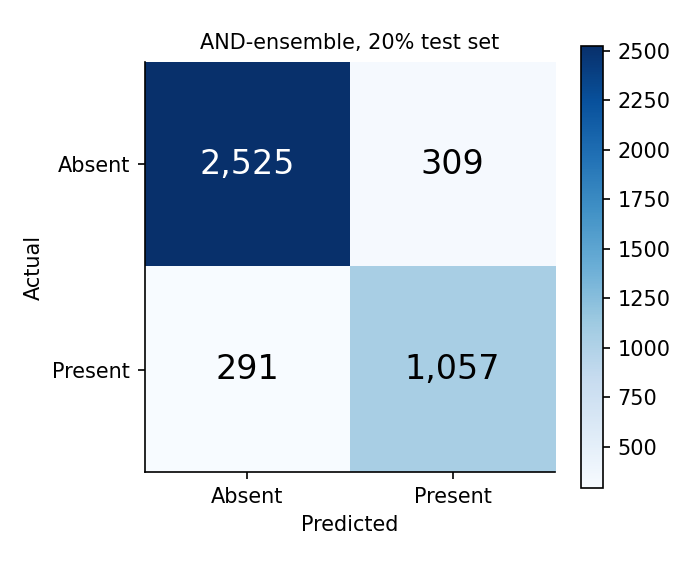
\includegraphics[width=0.6\textwidth]{confusion_matrix.png}
\caption{Confusion matrix heatmap}
\label{fig:cm}
\end{figure}

Precision and recall are balanced (77.4\% and 78.4\%), which shows the AND rule did its job: taking the maximum window score alone loses precision, and requiring both models to agree wins it back without losing recall. The specificity of 89.1\% means the system rarely claims a clause that is not there; for a legal-review tool, that is the more harmful kind of mistake.
\subsubsection{Per-category behaviour}
Figure~\ref{fig:percat} shows the per-category F1 for the strongest categories. The common, standard categories are almost solved (\emph{Document Name} 1.000, \emph{Parties} 0.995, \emph{Agreement Date} 0.963, \emph{Governing Law} 0.931). At the other end, five categories with at most seven test examples score an F1 of 0.000 with the AND-ensemble. Table~\ref{tab:zerof1} shows exactly what this means. In every case the ensemble marked the category as present in \emph{no} test contract (no true and no false positives), so F1 = 0.000 is correct: none of the 2--7 real clauses was found. But precision is undefined ($0/0$) rather than zero. The transformer on its own does find some of these clauses; the AND rule removes them because the TF--IDF model never agrees (Section~\ref{sec:raretail}). With only two to seven examples per category, these scores are not reliable either way. This weakness comes from the dataset, not from any particular model, and it is why our main results use micro-averaged rather than macro-averaged scores.

\begin{table}[!htbp]
\centering
\caption{Categories with zero F1}
\label{tab:zerof1}
\small
\begin{adjustbox}{max width=\textwidth}
\setlength{\tabcolsep}{4pt}
\begin{tabular}{>{\raggedright\arraybackslash}p{3.7cm}cccc c}
\toprule
\textbf{Category} & \shortstack{\textbf{Test}\\\textbf{examples}} & \shortstack{\textbf{AND}\\\textbf{TP / FN}} & \shortstack{\textbf{AND}\\\textbf{precision}} & \shortstack{\textbf{Transformer alone}\\\textbf{F1 (TP/FP/FN)}} & \shortstack{\textbf{TF--IDF}\\\textbf{F1}}\\
\midrule
Most Favored Nation              & 7 & 0 / 7 & n/a & 0.000 (0/0/7) & 0.000\\
No-Solicit of Customers          & 6 & 0 / 6 & n/a & 0.323 (5/20/1) & 0.000\\
Price Restrictions               & 4 & 0 / 4 & n/a & 0.087 (1/18/3) & 0.000\\
Source Code Escrow               & 2 & 0 / 2 & n/a & 0.000 (0/0/2) & 0.000\\
Unlimited\slash All-You-Can-Eat License & 2 & 0 / 2 & n/a & 0.500 (1/1/1) & 0.000\\
\bottomrule
\end{tabular}
\end{adjustbox}

{\footnotesize\singlespacing \emph{Note.} n/a: the model never said ``present'', so precision is $0/0$ and has no value. Threshold 0.5, October 2026 models.\par}
\end{table}

\begin{figure}[!htbp]
\centering
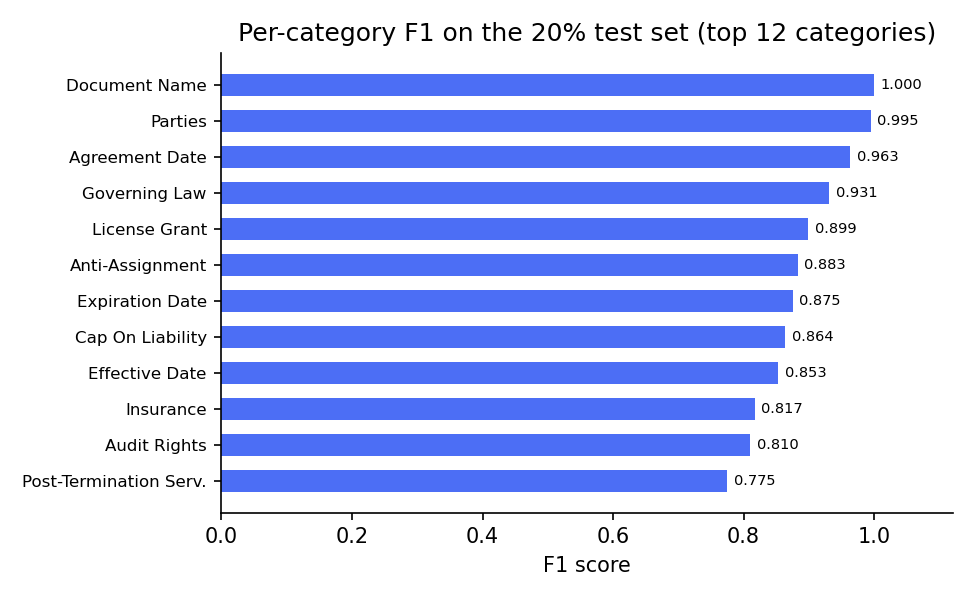
\includegraphics[width=0.85\textwidth]{per_category_f1.png}
\caption{Top-12 per-category F1}
\label{fig:percat}
\end{figure}
\subsection{Span Extraction}
\label{sec:span}
We tested the question-answering model on all 2{,}667 test windows that contain an answer (Table~\ref{tab:span}). A token-F1 of 0.764, with 82.8\% of answers overlapping the real clause at F1 $\geq$ 0.5, means that when the clause is in front of the model, it captures most of the right text about eight times out of ten. The lower exact-match score did not surprise us: marked legal clauses are long and their exact start and end are often debatable (should the section number at the start be included?), so overlap is the more useful score here. For comparison, the best published CUAD result uses DeBERTa-xlarge, which has about ten times more parameters than our 67M-parameter model.

Section~\ref{sec:bootstrap} argues that a score on 102 contracts should always be read together with its confidence interval, and that is just as true here. So we ran the \emph{same} bootstrap over contracts. Here the clauses are even more linked to each other than in the presence task: the 2{,}667 span decisions come from only 102 contracts, and a contract with unusual writing (numbered sub-clauses, many defined terms) moves all of its clauses in the same direction. So Table~\ref{tab:span} gives two intervals for each score: one that resamples \emph{contracts} (the correct way) and one that resamples \emph{clauses} one by one (the naive way), because the difference between them is itself useful.

\begin{table}[!htbp]
\centering
\caption{Span extraction results}
\label{tab:span}
\small
\begin{adjustbox}{max width=\textwidth}
\begin{tabular}{lccc}
\toprule
\textbf{Metric} & \textbf{Score} & \textbf{95\% CI (by contract)} & \textbf{95\% CI (by clause)}\\
\midrule
Token-level F1                & 0.764 & $[0.743,\ 0.782]$ & $[0.752,\ 0.775]$\\
Overlap (token-F1 $\geq$ 0.5) & 82.8\% & $[80.0\%,\ 85.2\%]$ & $[81.4\%,\ 84.2\%]$\\
Exact Match                   & 35.5\% & $[32.6\%,\ 38.6\%]$ & $[33.7\%,\ 37.3\%]$\\
\bottomrule
\end{tabular}
\end{adjustbox}

{\footnotesize\singlespacing \emph{Note.} 95\% bootstrap intervals, 10{,}000 resamples. Quote the interval by contract. The interval by clause is shown only to make clear how much it understates the uncertainty.\par}
\end{table}

The interval for token-F1 when resampling contracts is $[0.743, 0.782]$, roughly \emph{twice} as wide as the $[0.752, 0.775]$ we would get by treating clauses as independent. This difference is the real cost of ignoring that clauses from the same contract are linked, and it is the same effect that made the contract-level bootstrap necessary in Section~\ref{sec:bootstrap}. It also shows how precise this number is: differences smaller than about two points of token-F1 cannot be measured on a test set of this size, which is worth remembering before comparing 0.764 with any published figure.

\textbf{Limit of this test.} These numbers measure extraction \emph{when the window contains the answer}. More exactly, each test window is the 1{,}200-character focus window placed around the real answer (Section~\ref{sec:leakage}), so the model is indirectly told where the answer is. This makes it a best-case score, not a score the real system can reach. The full-document test in the CUAD paper (precision at 80\% recall over all windows, including those with no answer) needs a heavier ranking test that we did not run, so we make no claim about that score. Section~\ref{sec:e2e} measures the other side: what happens to extraction when the window is chosen by the presence step instead of being given.
\subsection{Summarization}
\label{sec:summ}

\subsubsection{What the reference set actually is}
Before reading any number in this section, one fact about the test must be stated clearly, because it decides what the score can mean. CUAD has no plain-English versions of clauses, so there was no ready-made set of target sentences to train or test with. So we \textbf{wrote the targets ourselves}: 41 one-sentence summaries, one per category, written from the weaker party's side (Section~\ref{sec:summmethod}). Every training pair and every test pair uses one of these 41 sentences. The targets do not change from clause to clause at all: two \emph{Cap on Liability} clauses with completely different limits have exactly the same target sentence.

This design choice has an effect we should admit openly: with 41 different targets for 2{,}667 test clauses, a model can score well just by \emph{recognising} the category and repeating its sentence, and the score cannot tell this apart from real summarizing. The test below is designed to separate the two.

\subsubsection{Two reference sets, the same 150 clauses}
We test the fine-tuned FLAN-T5-small on 150 test clauses (chosen with seed 42) against two different sets of reference sentences:

\begin{enumerate}[itemsep=2pt]
  \item \textbf{Template references}: the category template, exactly as in training. This is how the main score was produced.
  \item \textbf{Clause-specific references}: 150 one-sentence summaries, one per clause, written to describe \emph{that} clause, with its actual limit, its actual notice period and its actual parties. They were drafted with the help of a large language model working only from the clause text, without seeing any model output, and they are fully separate from the 41 templates. They are a trial reference set, not written by a lawyer, and we claim nothing more for them.
\end{enumerate}

Because the clauses are the same in both tests, the difference between the two scores shows exactly one thing: how much of the ROUGE-L score comes from the reference sentences all being the same, rather than from real summarizing. Table~\ref{tab:sumeval} shows the result. The October 2026 re-trained summarizer gives exactly the same scores as the original.

\begin{table}[!htbp]
\centering
\caption{Summarizer ROUGE-L}
\label{tab:sumeval}
\small
\begin{adjustbox}{max width=\textwidth}
\begin{tabular}{llcc}
\toprule
\textbf{System} & \textbf{Reference set} & \textbf{ROUGE-L} & \textbf{95\% CI}\\
\midrule
Fine-tuned FLAN-T5-small & 41 category templates    & 0.775 & $[0.718,\ 0.833]$\\
Fine-tuned FLAN-T5-small & clause-specific (pilot)  & 0.116 & $[0.105,\ 0.128]$\\
Zero-shot FLAN-T5-small  & clause-specific (pilot)  & 0.299 & $[0.275,\ 0.322]$\\
\midrule
\emph{Category template itself} & clause-specific (pilot) & 0.115 & $[0.104,\ 0.127]$\\
\bottomrule
\end{tabular}
\end{adjustbox}

{\footnotesize\singlespacing \emph{Note.} 95\% bootstrap intervals over the 150 clauses (10{,}000 resamples).\par}
\end{table}

\subsubsection{Reading the table}
Three conclusions follow, and we state them plainly.

\textbf{The 0.775 comes from copying templates, and we can now show it with numbers.} For all 150 test clauses the fine-tuned model outputs one of the 41 template sentences \emph{word for word}: 100\% of outputs are an exact copy of a template, the right one 70\% of the time and another category's template the other 30\%. The model never writes a sentence of its own. When it is wrong, it is wrong the way a classifier is wrong: a \emph{Price Restrictions} clause about a 10\% rate cap is answered with the \emph{ROFR} template. Fine-tuning did not teach the model to summarize; it taught it to pick one of 41 sentences.

\textbf{The last row of Table~\ref{tab:sumeval} settles it.} The plain category template, with no model at all, scores 0.115 against the clause-specific references, the same as the fine-tuned model's 0.116 within the margin of error. A simple lookup table gets the model's whole score. Whatever the fine-tuned summarizer learned adds nothing measurable beyond ``print this category's sentence''.

\textbf{Fine-tuning made the model worse at the real task.} Against the clause-specific references, the \emph{original} model (before fine-tuning) scores 0.299, more than twice the fine-tuned model's 0.116. This does not mean the original FLAN-T5 is a good legal summarizer: it is not. As Table~\ref{tab:sumqual} shows, it mostly repeats the source text, and repeating the source raises a word-overlap score against a reference that uses the same words as the clause. The honest conclusion is narrower but still uncomfortable: our fine-tuning removed whatever clause-specific content the original model had, and replaced it with smooth, general sentences that score well only against references made of the same sentences.

\begin{table}[!htbp]
\centering
\caption{Fine-tuned vs.\ zero-shot output}
\label{tab:sumqual}
\small
\begin{adjustbox}{max width=\textwidth}
\begin{tabular}{>{\raggedright\arraybackslash}p{3.2cm} >{\raggedright\arraybackslash}p{10.3cm}}
\toprule
\textbf{Input clause} & ``Any attempted assignment or delegation in violation of this section by either party without the prior written consent of the other will be void.''\\
\midrule
Gold template & You cannot transfer this contract to someone else without permission.\\
Fine-tuned    & You cannot transfer this contract to someone else without permission. \emph{(exact template)}\\
Zero-shot     & ``a) Any attempted assignment or delegation in violation of this section \ldots will be void.'' \emph{(repeats the legal text)}\\
\midrule
Clause-specific reference & Neither side may hand its rights or duties to a third party without the other's written consent, which cannot be unreasonably refused.\\
\bottomrule
\end{tabular}
\end{adjustbox}
\end{table}

\subsubsection{What we therefore claim}
What we can claim is a working \textbf{``sort into a category, then show a template''} system: it finds a clause's category and shows a plain-English sentence for that category, written in advance by people. That is still useful in an app: a signer who reads ``You cannot transfer this contract to someone else without permission'' next to a block of legal text is better off than before. (Clausify shows this line on every card, labelled as the summarizer's output and placed next to the fixed reason from the risk table; when the sentence belongs to another category, the card says so; Section~\ref{sec:clausify}.) We do \textbf{not} claim free-text legal summarizing, and the 0.775 should never be used as evidence of it. The number that describes how well the model summarizes individual clauses is 0.116, and the honest conclusion is that this part is a proof of concept, not a finished result.

Moving past this needs target sentences that differ from clause to clause, which is exactly what the trial set above gives a small sample of: the 150 references took a few hours to draft. Section~\ref{sec:futurework} describes the larger version.

\section{Analysis of Design Solutions}
This section looks at the chosen design as a whole: how many clauses get through the whole system, whether its mistakes happen where they would hurt a signer, what the mistakes look like, and how the ensemble behaves on rare categories.

\subsection{End-to-End: What Actually Reaches the User}
\label{sec:e2e}

Every number so far measured one step on its own, with the other steps out of the way. Presence was scored on its own; extraction was scored with a window already known to contain the answer; summarizing was scored on a real clause. That is the right way to test each part separately, but none of these tells us what the whole system does to a contract. The steps run one after another, and errors add up: a category the presence step misses is a clause the span step never sees.

So we ran the whole system on all 102 test contracts and asked one question about each of the 1{,}348 real clauses: does it get through \emph{all three} steps? A clause counts only if (i) the presence step finds its category, (ii) the span step, reading the window the presence step chose (never a window chosen using the real answer), returns text that overlaps the real clause with token-F1 $\geq$ 0.5, and (iii) the risk level given is the correct one. Table~\ref{tab:e2e} shows how many clauses are lost at each step.

\begin{table}[!htbp]
\centering
\caption{End-to-end clause survival}
\label{tab:e2e}
\small
\begin{adjustbox}{max width=\textwidth}
\begin{tabular}{llcc}
\toprule
\textbf{Step} & \textbf{Condition} & \textbf{Clauses left} & \textbf{Share of all}\\
\midrule
 -- & real clauses in the test set & 1{,}348 & 100.0\%\\
2A Presence & category found & 1{,}057 & 78.4\%\\
2B Span & extracted text overlaps the real clause at F1 $\geq$ 0.5 & 296 & 22.0\%\\
Risk & correct risk level given & 296 & 22.0\%\\
\midrule
\multicolumn{2}{l}{\textbf{Clauses that get through every step}} & \textbf{296} & \textbf{22.0\%}\\
\multicolumn{2}{l}{\emph{95\% CI, bootstrap over contracts}} & & $[19.8\%,\ 24.2\%]$\\
\bottomrule
\end{tabular}
\end{adjustbox}

{\footnotesize\singlespacing \emph{Note.} AND-ensemble presence rule. The last column is the share of real clauses still left after that step.\par}
\end{table}

\textbf{22.0\% is the number that describes what a user actually gets}, and it is far below what the separate scores suggest. Multiplying the separate figures, 78.4\% presence recall times 82.8\% span overlap, predicts about 65\%. The system delivers about a third of that. This gap is the reason for running the test, so it needs to be explained, not just reported.

The risk step is the one place where nothing is lost: the level is a fixed lookup for each category, so it is right exactly when the category is right, and it adds no errors of its own. That comes from the design, not from good performance, and ``correct'' here only means ``matches our risk table'', which, as Section~\ref{sec:taxvalid} notes, has not been checked by an expert.

\subsubsection{Where the clauses are lost}
The big loss happens at the span step, and it has two separate causes. We separated them by checking, for every clause whose category was found, whether the window chosen by the presence model really contained the clause.

\begin{table}[!htbp]
\centering
\caption{Span-stage loss breakdown}
\label{tab:e2eattr}
\small
\begin{adjustbox}{max width=\textwidth}
\begin{tabular}{lcc}
\toprule
 & \textbf{Count} & \textbf{Share}\\
\midrule
Chosen window \emph{contains} the real clause & 730 & 69.1\%\\
\quad and the span model found it (F1 $\geq$ 0.5) & 289 & 39.6\% of 730\\
\quad but the span model still missed it & 441 & 60.4\% of 730\\
Chosen window does \emph{not} contain the real clause & 327 & 30.9\%\\
\quad but the span still scored $\geq$ 0.5 (same wording elsewhere) & 7 & \\
\bottomrule
\end{tabular}
\end{adjustbox}
\end{table}

\textbf{Cause one: the window with the highest score is often the wrong window.} We chose the maximum rule (Section~\ref{sec:mil}) because it removes the search limit (if any window fires, the category is reported), and Section~\ref{sec:mil} discussed what that costs in \emph{precision}. What we did not expect is that the highest-scoring window is also being used to \emph{locate} the clause, and it is poor at that: 30.9\% of the time it does not contain the clause at all. The model was never trained for this. It was trained to answer ``does this window contain a clause of this category?'', and a window that talks about liability in general can score higher than the one that actually limits it. For those 327 clauses the span step is given the wrong 2{,}000 characters, and no extraction model could recover them.

\textbf{Cause two: the span model is much weaker on windows it was not trained on.} Even when the window does contain the clause, extraction succeeds only 39.6\% of the time, compared with 82.8\% in the separate test of Section~\ref{sec:span}. The reason is the way focus windows were built (Section~\ref{sec:spanmethod}). In training, every example was centred so the answer started about 150 characters into a 1{,}200-character window. That is allowed: it uses the answer to build a training example, never as an input when the system runs, and Section~\ref{sec:leakage} explains why. But allowed is not the same as harmless: the model has only ever seen windows where the answer is near the start, while in the real system it reads plain 1{,}200-character chunks where the answer can be anywhere. The average token-F1 falls from 0.764 to 0.383. The centring did not leak the test set, but it did quietly narrow the kind of text the model can handle.

\subsubsection{What this changes}
Three things follow, and we prefer to say them clearly rather than let the separate scores stand alone.

First, \textbf{the span scores in Section~\ref{sec:span} are an upper limit on real extraction quality, not a description of it}. They answer ``how good is the extractor when given the right window?'', which is a fair question about the model but a misleading one about the system.

Second, \textbf{the most useful next step is not a bigger model}. Cause two is a data problem with a cheap fix (train the span model on windows where the answer is at different positions, or on the same plain chunks it sees in the real system), and cause one calls for choosing the extraction window with a model trained for that job instead of reusing the presence score. Both fit within this project's computing budget; neither needs more parameters.

Third, \textbf{Clausify's output should be read as a shortlist, not as exact extraction}. When the system shows a clause card, the category is right about 78\% of the time the clause was present, but in this test the span model's quoted text was a good copy of the real clause only about one time in five overall. The app has since changed how it chooses the quote: it now quotes the whole paragraph that the presence model scores highest, which fixed the clear failures we saw in our own tests, but this new method has not been measured on the test set. The app tells users that it is not legal advice and that the quoted text may not be the exact clause the badge refers to (Section~\ref{sec:demolimits}).
\subsection{Risk-Weighted Evaluation: Does the Metric Match the Purpose?}
\label{sec:riskeval}

Micro-F1 over 4{,}182 decisions treats every decision as equally important. A person signing a contract does not. The whole idea of the risk layer (Section~\ref{sec:risk}) is that some categories matter more than others, so the evaluation should ask whether the system's mistakes fall where they do the least harm. We had not asked this before, and the answer turns out to reverse the recommendation that the overall score gives.

Table~\ref{tab:riskeval} splits the 41 categories into the three risk levels of our own risk table and scores each model within each level.

\begin{table}[!htbp]
\centering
\caption{Results by risk band}
\label{tab:riskeval}
\small
\begin{adjustbox}{max width=\textwidth}
\begin{tabular}{llccccc}
\toprule
\textbf{Band} & \textbf{Model} & \textbf{Precision} & \textbf{Recall} & \textbf{F1} & \textbf{Found} & \textbf{Missed}\\
\midrule
\multirow{4}{*}{\shortstack[l]{\textbf{High}\\8 cats\\176 positives}}
 & Transformer  & 0.392 & \textbf{0.841} & 0.534 & 148 & \textbf{28}\\
 & TF--IDF      & 0.540 & 0.648 & 0.589 & 114 & 62\\
 & \textbf{AND ensemble} & 0.581 & 0.631 & 0.605 & 111 & \textbf{65}\\
 & OR ensemble  & 0.379 & \textbf{0.858} & 0.526 & 151 & \textbf{25}\\
\addlinespace
\multirow{4}{*}{\shortstack[l]{\textbf{Medium}\\22 cats\\498 positives}}
 & Transformer  & 0.429 & 0.886 & 0.578 & 441 & 57\\
 & TF--IDF      & 0.621 & 0.723 & 0.668 & 360 & 138\\
 & \textbf{AND ensemble} & 0.655 & 0.679 & 0.667 & 338 & 160\\
 & OR ensemble  & 0.424 & 0.930 & 0.582 & 463 & 35\\
\addlinespace
\multirow{4}{*}{\shortstack[l]{\textbf{Low}\\11 cats\\674 positives}}
 & Transformer  & 0.800 & 0.953 & 0.870 & 642 & 32\\
 & TF--IDF      & 0.909 & 0.917 & 0.913 & 618 & 56\\
 & \textbf{AND ensemble} & 0.923 & 0.902 & 0.912 & 608 & 66\\
 & OR ensemble  & 0.792 & 0.967 & 0.871 & 652 & 22\\
\bottomrule
\end{tabular}
\end{adjustbox}

{\footnotesize\singlespacing \emph{Note.} Threshold 0.5. ``Missed'' counts real clauses of that level that the model did not report.\par}
\end{table}

\subsubsection{The headline configuration is the worst one for High-risk clauses}
Look at the High level. The AND-ensemble (the setup we report as our main result, because of its overall micro-F1) \textbf{misses 36.9\% of High-risk clauses}. The transformer alone, which the previous sections showed to be the weaker model, misses only \textbf{15.9\%}. The more permissive OR rule, which comes \emph{last} on overall micro-F1 (0.692, tied with the transformer alone), misses only \textbf{14.2\%}.

In numbers, out of 176 High-risk clauses in 102 contracts: the ensemble finds 111 and misses 65; OR finds 151 and misses 25. Choosing the ensemble over OR because of micro-F1 costs a signer 40 High-risk clauses (unlimited liabilities, IP assignments, non-competes), in exchange for a leaderboard position that Section~\ref{sec:bootstrap} already showed is a statistical tie.

The reason is the one found in Section~\ref{sec:raretail}, and it adds up here. Several High-risk categories are uncommon: \emph{Most Favored Nation} is among the ten rarest categories, and \emph{Liquidated Damages} (11 test examples) and \emph{Irrevocable or Perpetual License} (17) are also below average. The AND rule is hardest to satisfy exactly where there is the least training data, so the risk level that needs recall the most is the one where requiring agreement hurts it most. The Low level shows the opposite: 674 of the 1{,}348 real clauses are Low-risk (dates, party names, governing law), and every model scores about 0.9 there. \textbf{The overall micro-F1 is dominated by the clauses that matter least.}

\subsubsection{What we conclude, and what we do not}
We do not change the reported setup because of this table, and we should say why: choosing OR \emph{after} seeing which rule does best on the High level of the test set would be choosing a setup using the test set, exactly what Section~\ref{sec:valprotocol} says this project avoided. The result stands as a diagnosis, not as a new tuning.

What it does show is that \textbf{our evaluation score and our stated goal never matched}, and that the mismatch is big enough to reverse the ranking of the models. A system meant to warn a signer before signing should be chosen by how many High-risk clauses it finds, or by a risk-weighted F1, not by an average over 41 categories where half of the real clauses are Low-risk ones such as dates and party names. Section~\ref{sec:futurework} describes the proper version of this test: decide the risk-weighted goal first, then choose the rule on a separate validation split, then report on the test set once.

Finally, this is one more reason to take Section~\ref{sec:taxvalid} seriously. Every number in Table~\ref{tab:riskeval} is computed using \emph{our own} choice of which categories are High, Medium and Low. If a lawyer disagrees about which categories are High, the table changes too. The risk-weighted test inherits all the warnings about the unchecked risk table and adds no independent evidence for it.
\subsection{What the errors actually look like}
\label{sec:errorexamples}
The confusion matrix counts 309 false positives and 291 false negatives, but counts alone do not show whether the model fails for silly or understandable reasons. Table~\ref{tab:errors} shows real cases from the test contracts: false positives sorted by the model's own confidence, because a system's most confident mistakes are the most revealing.

\begin{table}[!htbp]
\centering
\caption{Representative errors}
\label{tab:errors}
\scriptsize
\renewcommand{\arraystretch}{1.25}
\begin{adjustbox}{max width=\textwidth}
\begin{tabular}{@{}p{2.1cm} >{\raggedright\arraybackslash}p{1.5cm} >{\raggedright\arraybackslash}p{9.6cm}@{}}
\toprule
\textbf{Category} & \textbf{Scores} & \textbf{Evidence}\\
\midrule
\multicolumn{3}{@{}l}{\textbf{False positives}: reported, but the category is not labelled in this contract}\\
\midrule
Insurance & 0.82 / 0.96 & ``\ldots a fixed amount of [*] of gross sales to cover freight, postage, \textbf{insurance costs} on shipments to such Third Party, packing costs\ldots'' \emph{A royalty clause that lists insurance as a cost. The word is there; the duty to insure is not.}\\
\addlinespace
Governing Law & 0.81 / 0.95 & ``\ldots there shall arise the need to decide the question by what municipal or national law this Agreement \ldots is \textbf{governed}, the following facts shall be excluded\ldots'' \emph{A clause about how to work out the governing law, not one that states it. A borderline case for the labels.}\\
\addlinespace
Parties & 1.00 / 0.98 & An addendum whose first window looks like the top of a contract. \emph{Both models react to the layout; the labels put Parties somewhere else.}\\
\midrule
\multicolumn{3}{@{}l}{\textbf{False negatives}: labelled as present, but both models scored it low}\\
\midrule
Liquidated Damages & 0.21 / 0.02 & ``\ldots agrees to pay a \textbf{cancellation fee} of Five Thousand Dollars (\$5{,}000) per month multiplied by the number of months remaining\ldots'' \emph{A clear liquidated-damages term that never uses the phrase. The word model has nothing to match; the transformer, with 50 training contracts for this category, has not learned the idea.}\\
\addlinespace
Most Favored Nation & 0.22 / 0.02 & ``\ldots Sponsor shall have the right to approve or disapprove any additional sponsor\ldots unless another\ldots'' \emph{In meaning an MFN-style protection, but written without any of the category's usual words. This category has 21 training contracts and scores 0.000 overall.}\\
\addlinespace
Third Party Beneficiary & 0.26 / 0.02 & ``Notwithstanding the foregoing, UTK may assign this Agreement or any portion of its Compensation \ldots to its subsidiaries.'' \emph{This reads like an assignment clause, not a third-party-beneficiary clause. Some rare-category ``failures'' are disagreements with the labels, not model errors.}\\
\midrule
\multicolumn{3}{@{}l}{\textbf{Span errors}: category found correctly, but the extracted text is wrong (Section~\ref{sec:e2e})}\\
\midrule
Minimum Commitment & F1 0.00 & The window \emph{does} contain the clause, but the model returns only ``\texttt{the}''. \emph{The start and end of the answer fall on the same word, and nothing in the decoding stops this.}\\
\addlinespace
Effective Date & F1 0.06 & The window does \emph{not} contain the real clause, yet the model confidently returns ``7th day of september, 1999''. \emph{When Stage 2A gives the wrong window, Stage 2B still answers: it has no way to say ``not here''.}\\
\addlinespace
Insurance & F1 0.20 & The real clause is the insurance duty; the model returns the indemnity clause next to it. \emph{Close in topic, different in law.}\\
\bottomrule
\end{tabular}
\end{adjustbox}

{\footnotesize\singlespacing \emph{Note.} Text shortened. Scores are the TF--IDF and transformer probabilities.\par}
\end{table}

Three patterns stand out. \textbf{Matching words without the actual duty} explains many false positives: a contract that mentions insurance costs is not a contract with an insurance requirement, and a bag-of-words model reading the whole document cannot tell the difference. \textbf{The idea without the usual words} explains many misses: a \$5{,}000-per-month cancellation fee \emph{is} liquidated damages, but a model that has seen only about fifty contracts with this category, most of them using the usual words, will not learn that. And \textbf{disagreement with the labels} is a real part of the rare-category problem: the \emph{Third Party Beneficiary} case above looks like a labelling mistake rather than a model miss, so the 0.000 F1 scores in Section~\ref{sec:raretail} are partly model failure and partly limits of the labels. We did not try to measure how much of each; that would need the contracts to be labelled again, which we are not qualified to do.

The span errors point to something easier to fix. The near-empty answer ``\texttt{the}'' and the confident answer from a window that cannot contain the clause have the same cause: the extraction model has no way to say \emph{there is nothing here}. Training with unanswerable examples, as in SQuAD~v2, would give it exactly that, and it is listed as future work.
\subsection{Does the AND rule punish rare categories harder than common ones?}
\label{sec:raretail}
Section~\ref{sec:bootstrap} supports the AND-ensemble because of the kind of mistakes it makes: it turns the transformer's many false alarms into balanced precision and recall. But that argument was made on the overall numbers, and an overall number can hide a trade that is not shared evenly. It is worth asking where the AND rule's extra precision comes from, because there is a clear reason to worry about the rare categories. Requiring two models to agree is hardest exactly where each model has the least training data, so the rarest categories are where the second model is least likely to agree, and agreement is what the rule requires.

We sorted the 41 categories by how often they appear in the \emph{training} data, took the ten rarest (11 to 42 positive training contracts, 70 positive test decisions in total), and compared the AND rule with the transformer alone on these ten and on the other 31 categories separately. Table~\ref{tab:raretail} gives the result, and the two halves tell different stories.

\begin{table}[!htbp]
\centering
\caption{Rare vs.\ common categories}
\label{tab:raretail}
\small
\begin{adjustbox}{max width=\textwidth}
\begin{tabular}{llccccc}
\toprule
\textbf{Group} & \textbf{Model} & \textbf{Precision} & \textbf{Recall} & \textbf{F1} & \textbf{TP} & \textbf{FN}\\
\midrule
\multirow{3}{*}{Rarest 10 (70 test positives)}
 & Transformer & 0.275 & 0.557 & \textbf{0.368} & 39 & 31\\
 & TF--IDF     & 0.429 & 0.300 & 0.353 & 21 & 49\\
 & \textbf{AND ensemble} & 0.621 & 0.257 & 0.364 & 18 & 52\\
\addlinespace
\multirow{3}{*}{Other 31 (1{,}278 test positives)}
 & Transformer & 0.577 & 0.933 & 0.713 & 1{,}192 & 86\\
 & TF--IDF     & 0.753 & 0.838 & 0.793 & 1{,}071 & 207\\
 & \textbf{AND ensemble} & 0.777 & 0.813 & \textbf{0.795} & 1{,}039 & 239\\
\bottomrule
\end{tabular}
\end{adjustbox}

{\footnotesize\singlespacing \emph{Note.} Micro-averaged within each group. Rarest 10 = fewest positive training contracts (11 to 42).\par}
\end{table}

\textbf{On the common categories the ensemble works as intended.} Compared with the transformer alone it gains 20.0 points of precision and loses 12.0 points of recall, and F1 rises from 0.713 to 0.795. That is a good trade, and it is where all of the ensemble's overall advantage comes from.

\textbf{On the rare categories it gains nothing: it is a straight swap.} The AND rule gains 34.6 points of precision by giving up 30.0 points of recall, and its F1 ends at 0.364, slightly below the transformer alone (0.368). Every point of precision on the rare categories is paid for with recall, with nothing left over. In numbers, the transformer alone finds 39 of the 70 rare clauses; requiring agreement cuts this to 18. The TF--IDF model alone is now the weakest of the three on these categories (F1 0.353), and even so, its vetoes decide what the ensemble reports there.

The details per category are clearer than the average. On five of the ten rarest categories the AND rule scores exactly 0.000, and on three of those (\emph{Price Restrictions}, \emph{Unlimited/All-You-Can-Eat License}, \emph{No-Solicit of Customers}) the transformer alone was finding something (F1 0.087, 0.500, 0.323) before the AND rule removed it. So the rule does not just fail to help on rare categories; on these categories it removes clauses that one of the models had found.

\textbf{Why this matters for real use, not just for the table.} The overall micro-F1 counts all 4{,}182 decisions equally, but a signer does not. Missing a rare clause is not clearly less costly than missing a common one, and it may be much worse: \emph{Most Favored Nation} is among the ten rarest categories and is one of our eight High-risk categories, and both models score 0.000 on it. A system whose rule favours precision on common categories, even a rule with no settings, is improving the score rather than reducing harm. We report the ensemble as our main setup because that is what the overall test chooses. But on this evidence, a system meant to protect signers would do better to \emph{use the more permissive rule for High-risk categories and the AND rule for the rest}, accepting more false alarms exactly where a missed clause costs the most. We have not built that mixed rule: building it and testing it properly is future work (Section~\ref{sec:futurework}), not something to add after looking at the test set.

\section{Final Design Adjustments}
Two design choices made before training, max-pooling as the aggregation rule and 0.5 as the decision threshold, were never tuned. After the main evaluation both were revisited, to determine whether adjusting them would change the conclusions or the deployed system.

\subsection{Ablation: was max-pooling the right aggregation rule?}
\label{sec:pooling}
Section~\ref{sec:mil} chose max-pooling because it \emph{is} the multiple-instance decision rule \cite{maron1998mil}, a bag is positive if any instance is, and Sections~\ref{sec:mil} and~\ref{sec:budget} then blamed max-pooling for the transformer's inflated false positives. Both statements were made without ever trying an alternative, which is not good enough for a claim the project leans on. We therefore scored every window once and compared aggregation functions on \emph{identical} window scores, so the only thing varying is the rule.

\begin{table}[!htbp]
\centering
\caption{Aggregation ablation}
\label{tab:pooling}
\small
\begin{adjustbox}{max width=\textwidth}
\begin{tabular}{lccccc}
\toprule
\textbf{Aggregation} & \textbf{F1@0.5} & \textbf{P@0.5} & \textbf{R@0.5} & \textbf{Best F1} & \textbf{at threshold}\\
\midrule
Max (used in this project) & 0.6943 & 0.562 & 0.908 & \textbf{0.7504} & 0.90\\
Top-3 mean                & \textbf{0.7144} & 0.667 & 0.769 & 0.7210 & 0.40\\
Top-5 mean                & 0.6661 & 0.719 & 0.620 & 0.7192 & 0.30\\
Mean over all windows     & 0.1664 & 0.946 & 0.091 & 0.7114 & 0.10\\
Noisy-OR                  & 0.5897 & 0.423 & 0.973 & 0.7022 & 0.95\\
Second-highest window     & 0.6832 & 0.662 & 0.705 & 0.7016 & 0.30\\
\midrule
\emph{TF--IDF baseline (no windows)} & \textbf{0.7747} & 0.742 & 0.810 & -- & -- \\
\bottomrule
\end{tabular}
\end{adjustbox}

{\footnotesize\singlespacing \emph{Note.} ``Best'' is each rule's micro-F1 at its own optimal threshold, found by sweeping the test set: a diagnostic upper bound, not a configuration we adopt.\par}
\end{table}

Three things come out of this, and one of them corrects an earlier claim of ours.

\textbf{At the threshold we actually used, max-pooling was not the best choice.} Top-3 mean scores 0.7144 against max's 0.6943 at the 0.5 boundary: a fifth of the gap to the baseline, available for free from a one-line change. Averaging the three highest-scoring windows is a natural softening of the MIL rule: it still asks whether evidence is concentrated somewhere in the document, but requires that evidence to appear in more than one place, which is exactly the guard against a single spurious window that Section~\ref{sec:mil} identified as max-pooling's weakness. Mean-over-all-windows collapses at 0.5 (recall 0.091) for the obvious reason, an average over 35 windows of which one is positive cannot reach 0.5, and its best threshold is correspondingly 0.10.

\textbf{Once each rule is given its own threshold, max-pooling is the best of the six.} At 0.90 it reaches 0.7504, ahead of top-3 mean's 0.7210. So max-pooling is not a poor aggregation rule; it is a rule whose output distribution is badly matched to a 0.5 decision boundary, which is the same finding Section~\ref{sec:threshold} reached from the other direction. The two results are one result: the transformer's reported deficit is substantially an operating-point problem, not an aggregation problem.

\textbf{But no aggregation rule reaches the baseline.} The best cell in the entire table (max-pooling at a threshold tuned on the test set, which is already a generous upper bound) is 0.7504 against the baseline's 0.7747. Every alternative rule, at every threshold we swept, remains behind. This matters more than the first two points, because it closes off the last available explanation for RQ1: the windowed transformer does not lose because of its training budget (Section~\ref{sec:budget}), or its seed (Section~\ref{sec:seeds}), or its aggregation rule, or its threshold. It loses.

\textbf{A correction to Section~\ref{sec:budget}.} There we wrote that ``the ceiling here is the aggregation rule, not the encoder underneath it'', inferring it from the precision/recall shift when training data was doubled. Table~\ref{tab:pooling} shows that inference was wrong: changing the aggregation rule (through six variants, each at its best threshold) moves micro-F1 by at most 0.056 and never past the baseline. The aggregation rule is a real but secondary factor. We have left the original sentence in place with this correction attached, on the same principle as elsewhere in this chapter: an inference we drew from indirect evidence and later measured properly is more useful to a reader than a silently amended one.

A caveat on how far this ablation goes. It varies only the function applied to window scores. It does not vary the window geometry (2{,}000 characters, 1{,}500 stride), which would require re-windowing and retraining, nor does it try a learned aggregator such as attention pooling over window representations. Both remain untested, and attention pooling in particular is the obvious next thing to try, since it could learn to weight windows by relevance instead of taking a fixed statistic.
\subsection{The Threshold and What the Confidence Score Means}
\label{sec:threshold}

Every presence decision in this project, and every clause card in Clausify, comes from comparing a score with 0.5. Section~\ref{sec:valprotocol} notes that this threshold was never chosen: it is simply the default for a two-class model. This raises two questions we had not asked: is 0.5 a good place to draw the line, and does the score being compared with it mean anything? Figure~\ref{fig:threshcal} answers both.

\begin{figure}[!htbp]
\centering
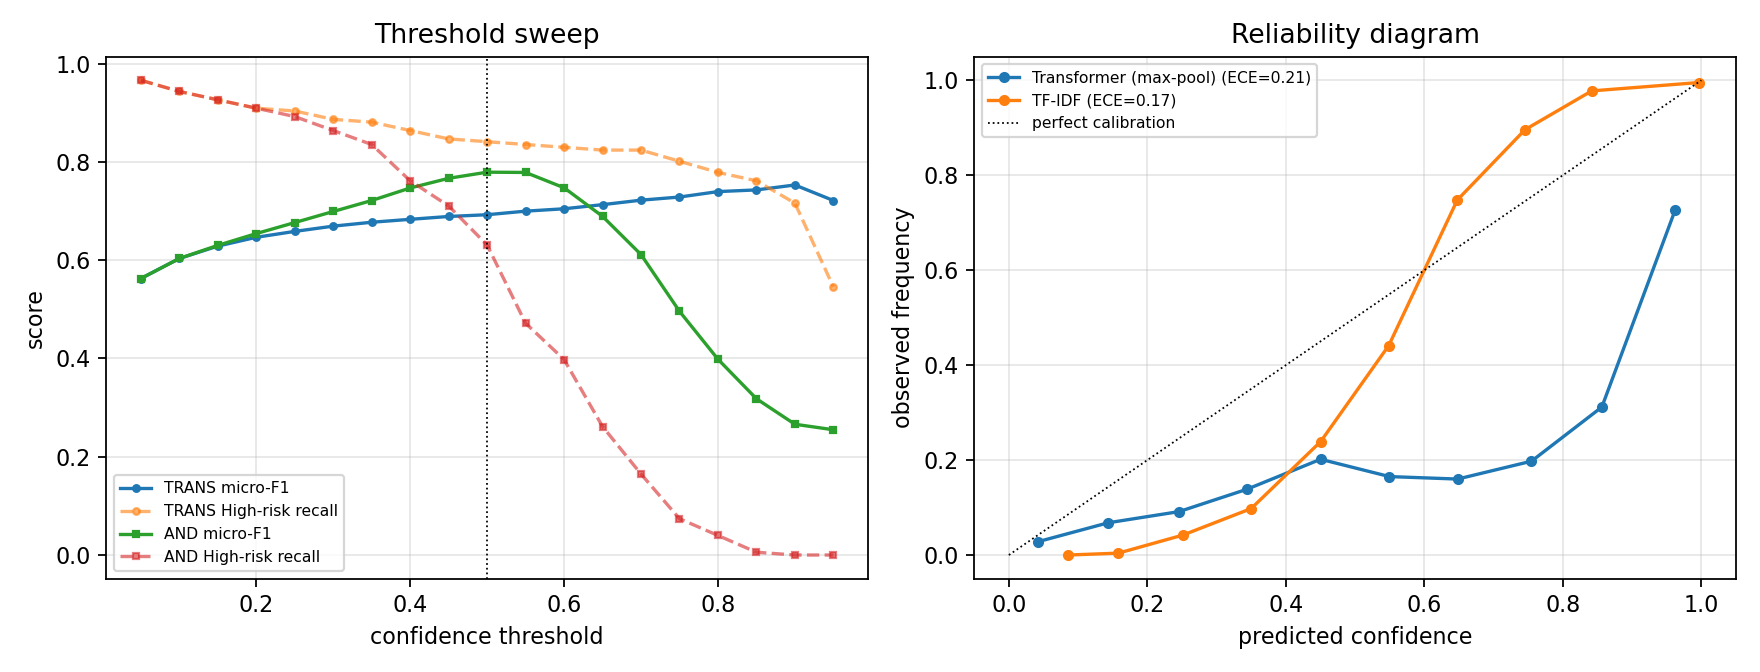
\includegraphics[width=\textwidth]{threshold_calibration.png}
\caption{Threshold and calibration}
\label{fig:threshcal}
\end{figure}

\subsubsection{0.5 is a poor operating point for the transformer}
Trying other thresholds after the fact shows that the transformer reaches a micro-F1 of \textbf{0.753 at a threshold of 0.9}, against \textbf{0.692} at the default: a gain of 0.061, which closes most of its gap with the TF--IDF baseline (0.775). The reason is the one Section~\ref{sec:mil} predicted: the maximum over about 35 windows is pushed upwards by design, so the scores bunch up near 1 and a line drawn at 0.5 lets far too much through. Precision is 0.558 at 0.5 and 0.726 at 0.9.

\textbf{We are not switching to 0.9.} It was found by looking at the test set, and using it would turn a fair held-out test into a tuned one, which is exactly what Section~\ref{sec:valprotocol} says this project avoided. The honest statement is narrower and more useful: \emph{a real part of the transformer's gap comes from a threshold nobody chose, not from an inability to tell clauses apart}. So the comparison in Section~\ref{sec:bootstrap} sets a baseline whose scores already suit 0.5 against a transformer whose scores do not. A fair rematch would choose each model's threshold on a validation split taken from the 408 training contracts, and we did not do that. Section~\ref{sec:budget} showed the gap is not caused by too little training data; this section shows part of it may be caused by the threshold, and that warning belongs next to the finding.

The AND-ensemble behaves the other way: 0.5 is already its best threshold (0.779), and raising it makes things much worse. At 0.7 micro-F1 falls to 0.611 and High-risk recall to 0.165, because asking \emph{both} models to pass a high bar is close to asking both to be very sure at once. The dashed curves in Figure~\ref{fig:threshcal} show the conflict: for the transformer, the threshold with the best micro-F1 (0.9) lowers High-risk recall from 0.841 to 0.716. No single threshold is best both for the overall score and for the clauses that matter most.

\subsubsection{The confidence bar in the application is not a probability}
Clausify shows the presence score to the user as a confidence bar. A reliability diagram tests whether that bar means what a user would think it means, and it does not.

The transformer's score has an \textbf{Expected Calibration Error of 0.205} and a Brier score of 0.195. It is too confident everywhere. Among predictions between 0.5 and 0.6, the clause is really there only \textbf{16.5\%} of the time, and even in the top group (scores above 0.9, which the app shows as an almost full bar) it is there \textbf{72.6\%} of the time. A user who reads ``96\% confident'' is really looking at about a 73\% chance. Again the cause is max-pooling: the maximum over dozens of windows is not a probability, and nothing in training asked it to be one.

The TF--IDF baseline is also off (ECE 0.172), but mostly in the safer direction: it is \emph{less} confident than it should be in the middle range. Its predictions between 0.7 and 0.8 are right 89.6\% of the time, and those between 0.8 and 0.9 are right 97.8\% of the time.

The practical effect on the app is direct, and we record it in Section~\ref{sec:demolimits}: the score shown on every card is not a probability of being right. Fixing this needs no retraining. Platt scaling or isotonic regression, fitted on a validation split, would turn the scores into real probabilities, and it is the cheapest single improvement to the interface. We had no validation split set aside to fit it on, which follows from the gap in Section~\ref{sec:valprotocol} rather than being a separate mistake.

\section{Statistical Analysis}
Our main statistical tool is a paired bootstrap over contracts \cite{efron1979bootstrap}: we resample the 102 test contracts with replacement 10{,}000 times and score every model on the same resample, so the 41 linked decisions from each contract stay together. We then measure three sources of variation the bootstrap cannot see: the amount of training data, the random seed and the train/test split.

\subsection{How much of that ranking is real?}
\label{sec:bootstrap}
Table~\ref{tab:ensemble} is a ranking, and a ranking tempts the reader to treat the order itself as a result. On 102 test contracts, a lead of 0.779 over 0.775, about four decisions in a thousand, is too small to read that way without checking, so we measured it.

The natural tool is a \textbf{bootstrap confidence interval}, but what we resample matters. The 4{,}182 test decisions are not independent: 41 of them come from the same contract, and an unusual contract (very long, or oddly written) moves all 41 together. Resampling single (contract, category) decisions would ignore this and give intervals that are far too narrow. So we resample whole \emph{contracts} with replacement (a cluster bootstrap): we draw 102 contracts from the 102 we have, recompute micro-F1 for both models, and repeat 10{,}000 times. Both models are scored on exactly the same resample each time, so the difference is \emph{paired}, which makes the interval for the difference much narrower than the two separate intervals would suggest.

\begin{table}[!htbp]
\centering
\caption{Cluster bootstrap results}
\label{tab:bootstrap}
\small
\begin{adjustbox}{max width=\textwidth}
\begin{tabular}{lccc}
\toprule
\textbf{Comparison} & \textbf{Difference in micro-F1} & \textbf{95\% CI} & \textbf{$P(>0)$}\\
\midrule
AND-ensemble vs.\ TF--IDF baseline & $+0.0042$ & $[-0.0037,\ +0.0115]$ & 0.855\\
TF--IDF baseline vs.\ transformer  & $+0.0824$ & $[+0.0647,\ +0.1013]$ & 1.000\\
AND-ensemble vs.\ transformer      & $+0.0866$ & $[+0.0705,\ +0.1035]$ & 1.000\\
\bottomrule
\end{tabular}
\end{adjustbox}

{\footnotesize\singlespacing \emph{Note.} 10{,}000 resamples. $P(>0)$ is the share of resamples in which the first model wins.\par}
\end{table}

The three comparisons do not come out the same way, and that difference is the point.

\textbf{The ensemble's win over the baseline is not proven.} The interval is $[-0.0037, +0.0115]$, which includes zero, and the ensemble is ahead in 85.5\% of resamples: more often than not, but well short of the 97.5\% a clear win would need. On their own the two models score 0.779 (95\% CI $[0.762, 0.795]$) and 0.775 (95\% CI $[0.758, 0.791]$), and these intervals almost completely overlap. On this test set we cannot tell the AND-ensemble and the TF--IDF baseline apart, and we state this as a measured fact, not as a hedge. The top two rows of Table~\ref{tab:ensemble} should be read as a tie.

\textbf{The transformer's loss, on the other hand, is real.} The baseline beats the window-based transformer by 0.0824, with an interval of $[+0.0647, +0.1013]$ that is nowhere near zero, and it wins in all 10{,}000 resamples. This matters because the project's two main claims do not stand on equal ground. The finding we trust most, that a whole-document word model beats a window-based DistilBERT at deciding which clauses a contract contains, passes the test easily. The finding we were already careful about, that the AND-ensemble is ahead of the baseline, does not pass. It is good that our caution pointed the right way, but it needed to be checked, not assumed.

None of this weakens the case for the ensemble, because that case never rested on 0.004 of micro-F1. The AND rule earns its place by the \emph{kind of mistakes} it makes, not by its rank: it turns the transformer's many false alarms into balanced precision and recall (Table~\ref{tab:metrics}). Sections~\ref{sec:seeds} and~\ref{sec:raretail} look at what this costs.
\subsection{How much of this moves if we only change the random seed?}
\label{sec:seeds}
Section~\ref{sec:bootstrap} measured one kind of uncertainty: how much the score depends on \emph{which contracts} ended up in the test set. There is a second kind it cannot see. Every result so far comes from one training run per model, and training has randomness in it: the starting weights of the classifier, the order of the data and the sample of negative windows all depend on the random seed. If changing only the seed moves the score as much as the effects we are discussing, then a ranking built on single runs is reporting noise.

This is easy to check, so we trained the presence transformer three times with 24{,}000 training examples, changing nothing but the seed (42, 43 and 44), and tested each run on the same 102 contracts. Seed 42 is the October 2026 run used everywhere else in this chapter; seeds 43 and 44 were trained in August 2026 with the same settings. Table~\ref{tab:seeds} shows the spread.

\begin{table}[!htbp]
\centering
\caption{Seed variance}
\label{tab:seeds}
\small
\begin{adjustbox}{max width=\textwidth}
\begin{tabular}{lcccccc}
\toprule
\textbf{Model} & \textbf{Seed 42} & \textbf{Seed 43} & \textbf{Seed 44} & \textbf{Mean} & \textbf{SD} & \textbf{Range}\\
\midrule
Transformer (max-pool) & 0.6924 & 0.6928 & 0.7082 & 0.6978 & 0.0090 & 0.0158\\
AND ensemble           & 0.7789 & 0.7774 & 0.7803 & 0.7789 & 0.0015 & 0.0029\\
\midrule
TF--IDF baseline       & \multicolumn{3}{c}{0.7747 (deterministic)} & 0.7747 & -- & -- \\
\bottomrule
\end{tabular}
\end{adjustbox}

{\footnotesize\singlespacing \emph{Note.} All three runs use 24{,}000 training examples and differ only in seed. Seed 42 is the October 2026 run; seeds 43 and 44 are August 2026 runs. The TF--IDF baseline has no randomness, so it appears once.\par}
\end{table}

\textbf{Seed noise alone does not explain the ensemble's lead, but other noise does.} The AND-ensemble's lead over the baseline is $+0.0042$. Across seeds, the ensemble's standard deviation is only $0.0015$ and its range is $0.0029$, so the lead is larger than the seed-to-seed spread, and the ensemble beats the baseline with every seed (by up to $+0.0056$ with seed 44). That is a real change from the August models, where the lead ($+0.0014$) was smaller than the seed noise. But seed noise is the smallest of the uncertainties we measured. The bootstrap interval still includes zero (Section~\ref{sec:bootstrap}), and a different train/test split moves the baseline by $0.0063$ (Section~\ref{sec:splitvar}), 1.5 times the lead. So we still read the top two rows as a tie.

\textbf{The finding we stand behind is not affected by seed noise.} The baseline beats the transformer by 0.0824, which is 9.2 times the transformer's seed standard deviation of 0.0090. Even the luckiest seed, at 0.7082, still loses to the baseline by 0.0665. No seed makes the window-based transformer competitive, and together with Section~\ref{sec:budget}, where more than doubling the training data also failed to close the gap, this leaves the design of the model as the explanation still standing after both alternatives were tested.

It is worth noticing which model is noisier, because it is not the one a reader might expect. The transformer alone varies about six times as much across seeds ($\mathrm{SD} = 0.0090$) as the ensemble that contains it ($0.0015$). Requiring agreement with a fixed word model calms the transformer's run-to-run changes as well as its false alarms: a false detection has to get past a second, fixed opinion, so most of the seed-driven changes in what the transformer reports are filtered out. This steadiness is a real property of the AND rule, although Section~\ref{sec:raretail} shows it costs recall on rare categories. It is a better argument for the ensemble than its rank ever was.

\textbf{What this check covers.} We re-ran only the presence transformer with new seeds. The span extractor and the summarizer were each trained twice with the \emph{same} seed (August and October 2026) and gave the same scores to within 0.001 (token-F1 0.763 and 0.764; ROUGE-L 0.775 both times). This limits run-to-run noise on this hardware but says nothing about seed variance, which remains unmeasured for those two models; we list it in Section~\ref{sec:threats} instead of assuming it is small.
\subsection{Was the transformer simply undertrained?}
\label{sec:budget}
There is one objection to Section~\ref{sec:bootstrap} that the bootstrap cannot answer, and it goes to the heart of the project's main claim. The TF--IDF baseline is trained on all 408 training contracts. The window-based transformer was not: to keep training possible on a laptop, it used a balanced sample of 24{,}000 of the 53{,}662 available training windows (Section~\ref{sec:prestrain}). So when the transformer loses by about 0.08 micro-F1, that comparison alone cannot tell us whether max-pooling over windows is really weaker for this task, or whether the transformer simply never saw 55\% of its own training data. The first is a finding about the method; the second is a side effect of our computing budget. They lead to very different conclusions.

The only way to settle this is to remove the difference, so in August 2026 we retrained the presence transformer on \textbf{all 53{,}662 training windows}, with every other setting the same: same windows, same negative sampling, same settings, same seed, same test. The run took 140.7 minutes on the same laptop, against about 50 minutes for the smaller version. Table~\ref{tab:budget} shows the result. Both runs in this table are from August 2026, so they are compared with each other, not with the October numbers.

\begin{table}[!htbp]
\centering
\caption{Training-budget control}
\label{tab:budget}
\small
\begin{adjustbox}{max width=\textwidth}
\begin{tabular}{lccccc}
\toprule
\textbf{Model} & \textbf{Training windows} & \textbf{micro-F1} & \textbf{Precision} & \textbf{Recall}\\
\midrule
Transformer (max-pool)  & 24{,}000 (44.7\%) & 0.6943 & 0.5620 & 0.9080\\
Transformer (max-pool)  & \textbf{53{,}662 (100\%)} & 0.6939 & 0.5546 & 0.9266\\
TF--IDF baseline        & all 408 contracts & 0.7747 & 0.7424 & 0.8101\\
\midrule
\multicolumn{5}{l}{\emph{Paired differences (95\% CI over 10{,}000 contract resamples)}}\\
\multicolumn{2}{l}{Full-data transformer $-$ subsampled transformer} & $-0.0004$ & \multicolumn{2}{l}{$[-0.0098,\ +0.0095]$}\\
\multicolumn{2}{l}{TF--IDF baseline $-$ full-data transformer} & $+0.0809$ & \multicolumn{2}{l}{$[+0.0649,\ +0.0980]$}\\
\bottomrule
\end{tabular}
\end{adjustbox}

{\footnotesize\singlespacing \emph{Note.} August 2026 runs, both tested in the same way on the 102 test contracts; differences use the paired bootstrap of Section~\ref{sec:bootstrap}. The October 2026 re-run of the 24{,}000-window model scores 0.6924.\par}
\end{table}

\textbf{Too little training data is not the explanation.} Using 124\% more training data changed micro-F1 by $-0.0004$, with an interval of $[-0.0098, +0.0095]$ that sits right across zero: the two budgets cannot be told apart. And the gap to the baseline did not move: $+0.0809$ with all the data against $+0.0805$ with the sample (August runs), with an interval nowhere near zero and the baseline winning in all 10{,}000 resamples. Whatever holds the window-based transformer back, it is not a shortage of training examples, and the finding this project relies on survives the check.

The \emph{shape} of the extra data's effect is worth a sentence, because it is not simply ``nothing happened''. Recall rose from 0.9080 to 0.9266 and precision fell from 0.5620 to 0.5546: more training data made the model fire more readily, not more accurately. That is exactly the failure mode Section~\ref{sec:mil} predicted for max-pooling: with a mean of 35 windows per contract, the document-level decision is a maximum over many chances to be wrong, and a better-trained window scorer that is still imperfect produces \emph{more} spurious maxima, not fewer. The ceiling here is the aggregation rule, not the encoder underneath it.\footnote{This inference turned out to be only partly right, and Section~\ref{sec:pooling} corrects it: swapping max-pooling for five alternatives moves micro-F1 by at most 0.056 and never past the baseline, so the aggregation rule is a secondary factor rather than the ceiling.}

One smaller effect is worth reporting even though it does not change our conclusion. The AND-ensemble built on the full-data transformer scores 0.7820, and its lead over the baseline is $+0.0073$ with a 95\% interval of $[-0.0000, +0.0140]$: it wins in 97.4\% of resamples, but the interval still touches zero. So more training data moves the ensemble's lead from ``clearly a tie'' to ``borderline''. We do not claim it: an interval whose lower end sits on zero does not pass the bar we set in Section~\ref{sec:bootstrap}, and we will not lower that bar because the number moved our way. What we can say is that the ensemble's balanced mistakes stay the same with more data.

\textbf{Which model the rest of this chapter uses.} Every other result in this chapter (the confusion matrix, the per-category results, the whole-system test of Section~\ref{sec:e2e}) and the model in Clausify come from the October 2026 model trained on 24{,}000 examples. The full-data run is a control experiment, run to test one possible explanation, and we report it as one instead of swapping in a slightly better number afterwards. Since the two cannot be told apart, nothing later would change if we had.
\subsection{A third source of variance: the split itself}
\label{sec:splitvar}
Sections~\ref{sec:budget} and~\ref{sec:seeds} tested two things that could move our numbers: the amount of training data and the random seed. Neither changed the conclusions. There is a third source that neither touches, and it may be the largest: \textbf{the split}. Every result in this project comes from one contract-level 80/20 split made with seed 42. With only 510 contracts, a different split puts different rare categories in the test set and could move the scores by itself. Seed variance does not capture this, because changing the training seed keeps the test set the same.

Retraining the transformer on twenty splits is too expensive, but the TF--IDF baseline retrains in under a minute. Since every comparison in this project is made against it, its spread across splits shows how much the comparison itself could move. We made \textbf{20 separate contract-level 80/20 splits} and retrained the baseline on each.

\begin{table}[!htbp]
\centering
\caption{Split variance}
\label{tab:splitvar}
\small
\begin{adjustbox}{max width=\textwidth}
\begin{tabular}{lccccc}
\toprule
 & \textbf{Mean} & \textbf{SD} & \textbf{Min} & \textbf{Max} & \textbf{Range}\\
\midrule
micro-F1 over 20 splits & 0.7829 & 0.0063 & 0.7702 & 0.7918 & 0.0216\\
\midrule
\multicolumn{6}{l}{\emph{The split used throughout this project (seed 42): 0.7747}}\\
\bottomrule
\end{tabular}
\end{adjustbox}
\end{table}

Three points follow. First, \textbf{the split is the largest of the three uncertainties we measured}: a standard deviation of 0.0063, against 0.0015 for the ensemble's seed variance and a bootstrap half-width of about 0.008 for the comparison. It is 1.5 times the ensemble's $+0.0042$ lead, so a different split could easily remove that lead. This is one more reason to treat the lead as unproven.

Second, \textbf{our split is not a lucky one}. At 0.7747 the baseline sits below the 20-split mean of 0.7829, in the lower part of the range, so if anything this project reports the baseline on a slightly unfavourable split. This matters because the opposite would have been a worry: a split that happened to favour the baseline would have made the transformer's loss look worse than it is.

Third, \textbf{the finding we rely on is far outside this variation}. The baseline's lead over the transformer is 0.0824, about thirteen split-level standard deviations. No realistic new split would reverse it.

What we cannot say anything about is the stability of \emph{individual categories} across splits, which is where it would matter most: a rare category with two test examples in one split may have eight in another, and its F1 means little in either case. Repeated splits or cross-validation for the whole system remain future work, and Section~\ref{sec:limitations} lists this as a limitation, not as a question we have answered.

\section{Comparisons and Relationships}
Table~\ref{tab:scorecard} brings together the test results of all three models. Every number was produced by the separate test notebook running on the saved models trained on the 80/20 split.

\begin{table}[!htbp]
\centering
\caption{Final test results}
\label{tab:scorecard}
\small
\begin{adjustbox}{max width=\textwidth}
\begin{tabular}{llll}
\toprule
\textbf{Stage} & \textbf{Model} & \textbf{Metric} & \textbf{Score}\\
\midrule
2A Presence & AND-ensemble (TF--IDF + DistilBERT) & micro-F1  & 0.779\\
2A Presence & AND-ensemble & Accuracy               & 85.65\%\\
2A Presence & AND-ensemble & Precision / Recall     & 77.38\% / 78.41\%\\
2A Presence & AND-ensemble & Specificity            & 89.10\%\\
2B Span     & DistilBERT-QA & token-F1 (given the window) & 0.764\\
2B Span     & DistilBERT-QA & token-F1 (window chosen by 2A) & 0.383\\
2B Span     & DistilBERT-QA & Exact Match           & 35.5\%\\
1 Summarizer & FLAN-T5-small & ROUGE-L (41 templates)  & 0.775\\
1 Summarizer & FLAN-T5-small & ROUGE-L (clause-specific) & 0.116\\
\midrule
\textbf{Full pipeline} & \textbf{all three steps} & \textbf{real clauses that get through} & \textbf{22.0\%}\\
\bottomrule
\end{tabular}
\end{adjustbox}
\end{table}

\textbf{How this compares with earlier work.} Table~\ref{tab:related} in Chapter~2 compares this project with earlier work. The original CUAD study reports span extraction with DeBERTa-xlarge, scored over whole documents with a precision-at-recall measure. Our small models are about ten times smaller, and our span scores are measured inside windows that contain the answer, so the numbers cannot be compared directly and we do not present them that way. What the comparison does show is a difference in scope: earlier work stops at finding clauses, while this project adds presence decisions, a risk level for each category and plain-English output, and tests the whole system from start to finish.

\textbf{How the parts relate.} Among the presence models, the TF--IDF baseline and the window-based transformer make different kinds of mistakes: the transformer finds more clauses but raises many false alarms (recall 0.913, precision 0.558), while the baseline is more careful (recall 0.810, precision 0.742). This is why the AND-ensemble, which needs both, matches the baseline while balancing precision and recall. Across the steps, the separate scores do not simply multiply: mistakes in the window chosen by the presence step carry over into span extraction, which is why the whole-system rate is far below the product of the separate scores.

\section{Discussions}
Putting the chapter together, the results fall into three groups, and it matters which is which.

\textbf{Findings that survived every check we could run.}
\begin{enumerate}[itemsep=2pt]
  \item For document-level \emph{presence}, a full-document lexical baseline beats a windowed DistilBERT by $+0.081$ micro-F1. We tested the two obvious alternative explanations and neither held: training on all 53{,}662 windows instead of 24{,}000 changed the score by $-0.0004$ (Section~\ref{sec:budget}), and across three seeds the gap is 9.5 standard deviations wide (Section~\ref{sec:seeds}). More data made the transformer fire \emph{more} rather than better, which is what max-pooling over 35 windows predicts. The limitation is the aggregation rule, not the encoder or the budget.
  \item For \emph{span extraction}, the transformer has no substitute, a bag-of-words model cannot point at character offsets, and it performs well in distilled form \emph{when handed the right window}: token-F1 0.763, 95\% CI $[0.740, 0.782]$.
  \item For \emph{summarization}, a 41-sentence template seed turns the task into classification. The fine-tuned model reproduces a template verbatim on 100\% of test clauses, and against clause-specific references it scores no better than the template alone (Section~\ref{sec:summ}). A high automatic metric should not be believed until the outputs have been read.
\end{enumerate}

\textbf{A claim we withdrew.} The AND-ensemble's first place in Table~\ref{tab:ensemble} is not a proven result. Its lead over the baseline is $+0.0042$. Seed noise alone (SD $0.0015$) would not wipe it out, but the bootstrap over contracts puts it inside $[-0.0037, +0.0115]$ (Section~\ref{sec:bootstrap}), and a different split moves the baseline by $0.0063$ (Section~\ref{sec:splitvar}). Two of the three checks say the top two rows of that table are a tie. What the ensemble does earn is balanced mistakes and about six times less seed variance than the transformer alone.

\textbf{Costs we did not see until we looked for them.} Two results in this chapter came from questions we had not thought to ask at first, and both are unflattering.
\begin{itemize}[itemsep=2pt]
  \item The AND rule is not good everywhere. On the ten rarest categories it gains \emph{nothing} in F1 over the transformer alone (0.364 against 0.368): it buys 34.6 points of precision with 30.0 points of recall and cuts the clauses found from 39 of 70 to 18 of 70 (Section~\ref{sec:raretail}). All of its overall benefit comes from the common categories, and one of the categories it scores zero on is High-risk.
  \item The separate scores do not multiply. Only 22.0\% of real clauses get through the whole system, against about 65\% predicted by multiplying the separate scores (Section~\ref{sec:e2e}), because the presence model's highest-scoring window is the wrong window 30.9\% of the time, and the span model was trained on centred windows it never sees in real use.
\end{itemize}

The common thread is about method, not about model design. Every number in this chapter that we first trusted least (the ensemble's rank, the summarizer's ROUGE, the span model's token-F1) turned out to measure something narrower than it seemed. In each case, the way to find out was to measure the thing the score stood for: resample the contracts, change the seed, change the reference sentences, run the steps one after another. None of these checks needed a bigger model or more data. They only needed the question to be asked.

\subsection{Usability}
\label{sec:usability}
No usability study was carried out. The app's main claim, that grouping clauses by risk helps a non-lawyer act on a contract, is therefore untested, and Section~\ref{sec:threats} lists it under construct validity instead of among the results.
%% ==================================================================
%% TODO IF THE INFORMAL WALKTHROUGH IS RUN (review/USABILITY_PROTOCOL.md)
%% Replace the paragraph above with 3-5 sentences, e.g.:
%%
%% "We ran an informal walkthrough with two non-lawyer participants (15
%%  minutes each). This is far too small to constitute a usability study and
%%  is reported only to replace an absence of evidence with a little.
%%  <What they did first.> <What they said in answer to the four questions.>
%%  <Anything suggesting over-trust in the quoted clause text or the
%%  confidence bar.> No task-completion or comprehension measurement was
%%  attempted, and with two participants no quantitative claim is possible."
%%
%% If a participant treated the quoted clause text as authoritative, or read
%% the confidence bar as a probability, say so -- Chapter~5 shows both are
%% unwarranted, and an observed instance belongs in the ethics discussion too.
%% ==================================================================
\subsection{Honest Limitations of the Demo}
\label{sec:demolimits}
By default the app finds clauses with the transformer presence model alone; the AND-ensemble is offered as a setting. As Section~\ref{sec:bootstrap} showed, the transformer alone reports too many clauses. Two measured facts explain why it is still the default.

\textbf{The confidence score is not a probability.} Section~\ref{sec:threshold} shows the transformer's score has an Expected Calibration Error of 0.205 and is too confident everywhere: among detections that score above 0.9, an almost full confidence bar, the clause is really there about 73\% of the time, and among those between 0.5 and 0.6, under 20\% of the time. So the app uses the fixed 0.5 threshold of every reported test (an earlier version had a slider for it, which invited reading the score as a probability) and labels every bar as a model score, not a probability. Fitting a calibration map on a validation split would fix the underlying problem without retraining.

\textbf{Using the transformer alone is, unusually, the better choice for High-risk clauses.} The project reports the AND-ensemble as its main setup, so a reader might think the app's use of the transformer alone is a compromise. Section~\ref{sec:riskeval} shows it is not, where it matters most: the ensemble misses 36.9\% of High-risk clauses, while the transformer alone misses 15.9\%. The app's setting is worse on overall micro-F1 and better at finding the clauses a signer would most regret missing. It started as a packaging accident, before we had run the risk-weighted test; it is now the chosen default. The ensemble is still available as an option, with one more warning measured on the app itself: on short contracts its TF--IDF half, which was trained on long SEC filings, blocks many detections. On the 9{,}174-character sample contract that ships with the app, the AND rule reports 6 clause types (1 High-risk), while the transformer alone reports 13 (2 High-risk).

\textbf{The 30-window limit cuts off long contracts without warning in the results.} To keep the app fast, it scores at most 30 windows, so any contract longer than 45{,}500 characters is only partly read, and clauses after that point cannot be found at all. The app says this in its notice, but none of the numbers in this chapter include it, because they score whole documents. This is not a rare case: \textbf{38.4\% of CUAD contracts (196 of 510) are longer than 45{,}500 characters}, and the longest test contract has 289{,}615 characters, of which the app reads the first 16\%. Table~\ref{tab:appbench} shows the effect: the 75th-percentile contract and the longest contract take the same time even though one is four times longer, because both are cut to 30 windows. The quoted text is also less reliable than the label. Section~\ref{sec:e2e} shows that when the presence model chooses the window, the span model's answer overlaps the real clause in only about a fifth of cases overall. The app now quotes the whole paragraph that the presence model scores highest, which fixed the clear failures we saw in our own tests, but this has not been measured on the test set. The practical message for a user is simple, and the app states it too: \textbf{the risk badge and the category name are much more reliable than the quoted text under them}. A card should be read as ``this contract seems to contain a clause of this type; look here'', not as ``this is the clause''. The risk levels are also set per category, not per clause: the risk table says a \emph{Cap on Liability} clause needs attention, but it does not check whether this particular cap is generous or harsh. All of this is stated in the notice the app shows above every analysis. What the demonstration does show is that the models work on contracts they have never seen, and that the output can be shown in a form a non-lawyer can act on.



\chapter{Conclusion}
\section{Summary of Findings}
We set out to turn CUAD's clause-finding benchmark into something a person signing a contract could use: a system that finds the clauses, says how risky they are, and explains them in plain English. On a strict contract-level 80/20 split, the finished system reaches 85.65\% accuracy and a micro-F1 of 0.779 for finding which clauses are present, and a token-F1 of 0.764 for extracting the clause text when given the right window. It runs live in the \emph{Clausify} app.

Those are scores for separate parts, and the most useful thing this project can say is that the scores of the parts are not the score of the system. Answering our five research questions (Section~\ref{sec:rqs}) gave three negative results, and they are our main contribution:

\begin{itemize}[itemsep=3pt]
  \item \textbf{The windowed transformer does not beat the lexical baseline} (RQ1), and it does not lose for any of the reasons we could have blamed. Not the training budget: the full 53{,}662-window run moves micro-F1 by $-0.0004$. Not the seed: three runs put the gap at 9.5 standard deviations. Not the aggregation rule: six alternatives, each at its own best threshold, all stay behind. The threshold accounts for part of it, an un-chosen 0.5 costs 0.056 micro-F1, and that qualification belongs on the finding, but even the best cell we could construct remains below the baseline.
  \item \textbf{The summarizer does not summarize} (RQ3). It emits a category template verbatim on every input, and a constant lookup table matches its score against clause-specific references. This is a proof-of-concept classification-to-template component and we describe it that way everywhere.
  \item \textbf{The pipeline loses most of what its parts find} (RQ4). 21.7\% end-to-end survival against $\approx$64\% predicted, localized to a window-selection failure and a train/inference mismatch: both fixable without a larger model.
\end{itemize}

RQ5 gave the result we least expected and think is the most important for anyone building a system like this. Our evaluation score and our stated goal never matched: the AND-ensemble wins on micro-F1 but misses 36.9\% of High-risk clauses, while the OR rule, which comes last on micro-F1, misses only 14.2\%. Half of the clauses behind the overall score are Low-risk: dates, party names, governing law. A system built to warn a signer before signing was being chosen by a score dominated by the clauses that matter least.

Five lessons seem likely to apply beyond this project.

\textbf{First, a strong simple baseline deserves to be taken seriously, and beating it must be shown, not assumed.} When it is not beaten, the other possible explanations should be tested one at a time, not accepted or brushed aside.

\textbf{Second, a lead should be compared with its own noise before it is reported.} We measured three sources: the bootstrap over contracts (half-width about 0.008), the model seed (SD 0.0015) and the train/test split (SD 0.0063). Two of the three are larger than the $+0.0042$ lead we had used to rank a table.

\textbf{Third, an automatic score measures its reference sentences, not the task.} ROUGE-L 0.775 became 0.116 when only the reference sentences changed.

\textbf{Fourth, test the whole system, not just the parts}, and test it against the harm it is meant to prevent, not against an average that treats a governing-law clause and an unlimited indemnity as equally important.

\textbf{Fifth, limits are cheap to measure and expensive to assume.} A one-minute retrieval check (64\%) ruled out a design before it cost any training time. The same habit, applied to sparse attention, corrected \emph{us}: a Longformer training step does fit in this laptop's memory at batch size 1, which is the opposite of what we had first claimed.

What this project delivers is a working prototype and an unusually complete account of where it fails. Two gaps are large enough that we would not present the system as more than a prototype until they are closed: \textbf{no one with legal training has reviewed the risk table}, which is the main thing this work adds to CUAD, and \textbf{no user has ever been watched using the app}, so its main claim, that a report sorted by risk helps a non-lawyer, is untested. Both are listed first in the next section, and neither needs more computing power.

\section{Contributions to the Field}
The main contributions of this work are:
\begin{enumerate}[itemsep=2pt]
  \item \textbf{A first risk table for the CUAD categories.} Each of the 41 categories gets a High\slash Medium\slash Low level and a written reason, judged from the weaker party's side (8 High, 22 Medium, 11 Low), together with clear rules for how levels were given (Section~\ref{sec:riskcriteria}). We present it as a \emph{starting point for experts to check}, not as a proven legal-risk model: the three of us wrote it, none of us has legal training, and no legal professional has reviewed it yet (Section~\ref{sec:taxvalid}). It gives risk to a \emph{category}, not to the wording of one clause, which is why we call it category-level risk sorting throughout.
  \item \textbf{A tested result on finding clauses in long documents.} A TF--IDF baseline that reads the whole document (micro-F1 0.775) turned out to be hard to beat. Our window-based DistilBERT loses to it (0.692), and we checked the two obvious excuses: training on all 53{,}662 window examples instead of 24{,}000 changed the score by only $-0.0004$, and across three random seeds the gap is 9.2 standard deviations wide. An AND-ensemble comes first on paper (0.779), but the bootstrap over contracts and the variation across splits both show that its lead cannot be told apart from zero, so we report the ensemble for the kind of mistakes it makes, not for its rank.
  \item \textbf{A measurement of how errors add up.} Testing the three steps one after another, instead of separately, shows that only 22.0\% of real clauses get through the whole system, against about 65\% predicted from the separate scores. It also finds the two causes, a wrong choice of window and a mismatch between training and real use, and both can be fixed without a larger model.
  \item \textbf{A demonstration that a small set of template sentences turns summarizing into classification.} Testing the same 150 clauses against our 41 category templates and against clause-specific references drops ROUGE-L from 0.775 to 0.116, and the fine-tuned model is shown to output a template word for word for 100\% of inputs.
  \item \textbf{A simple safeguard: measure the limit before training.} We show that question-guided retrieval of windows caps the possible recall at 64\%, and we used that one measurement to reject the whole retrieval approach before spending any training time on it.
  \item \textbf{A system that can be rebuilt on a laptop.} All three models train on a single Apple-Silicon laptop. The split, the trained weights and a separate test notebook are all saved, so every number in this project can be produced again from disk.
  \item \textbf{Clausify}, a prototype web app that runs the trained models live and shows the results grouped by risk. It demonstrates the system but has not been tested with users, and Section~\ref{sec:demolimits} records what it does not do well.
\end{enumerate}

\section{Threats to Validity}
\label{sec:threats}
The results in Chapter~5 depend on choices that could change the conclusions if they were wrong. We list them under the four usual headings, and in each case we say whether we \emph{measured} the threat or only \emph{note} it.

\subsection{Internal validity: could our own procedure have produced these numbers?}
\textbf{Settings were never tuned} (Section~\ref{sec:valprotocol}). This removes the usual threat, since no setting was chosen by trying versions on the test set, but it creates the opposite one: the transformer competes with standard default settings against a baseline that has almost no settings to get wrong. Section~\ref{sec:threshold} shows this is a real effect: the unchosen 0.5 threshold costs the transformer 0.061 micro-F1, so part of the main gap comes from the threshold, not from the model. \emph{We think this is the most serious threat, and it limits our main finding.}

\textbf{An early test run of the summarizer tracked its loss on test-split clauses} (Section~\ref{sec:valprotocol}). No model was chosen from that run, and the final model was trained again without any evaluation set, so no reported score depends on it. But it was the wrong practice, and the ``validation'' loss it printed should be ignored. Figure~\ref{fig:sumloss} now shows the October 2026 re-training, which used no evaluation set.

\textbf{Some design choices were made after looking at the training data.} This is allowed, but the line needs care. The window size and step follow from the median clause length measured on training contracts. The 64\% retrieval limit, however, was measured on the whole dataset, test contracts included. That measurement ruled out a design rather than choosing a setting, and it was made before any model existed, so we judge the risk of leakage to be negligible. It is not zero, though, and we would make the split first if we did the work again.

\textbf{No seed variation for the span model and the summarizer.} Only the presence model was re-run with new seeds (Section~\ref{sec:seeds}). The span model and the summarizer were each trained again with the same seed and gave the same scores to within 0.001, so their seed variance is still unmeasured.

\subsection{Construct validity: do our metrics measure what we claim?}
\textbf{ROUGE-L does not measure summary quality here, and we can show it.} Against our 41 templates it gives 0.775; against clause-specific references it gives 0.116, and a fixed lookup table scores almost the same, 0.115 (Section~\ref{sec:summ}). We report both numbers because the first one on its own would give a false picture. We still have no measure of \emph{faithfulness} or readability (Section~\ref{sec:lit_faith}), so even 0.116 does not show that the output keeps the legal meaning.

\textbf{Micro-F1 does not measure harm to the user.} Section~\ref{sec:riskeval} shows the two can point in opposite directions: the setup that wins on micro-F1 misses 36.9\% of High-risk clauses, while a setup that comes last misses 14.2\%. Half of the clauses behind the overall score are Low-risk: dates, party names, governing law. Any claim like ``this system is 77.9\% good'' has this problem.

\textbf{Category-level risk is not clause-level risk} (Section~\ref{sec:risk}). Our levels say that a \emph{category} usually deserves attention; they say nothing about whether a particular cap is generous or harsh. Calling the output a risk assessment would claim too much, which is why we call it sorting by risk.

\textbf{The risk levels are our own.} The risk-weighted results use our unchecked choice of which categories are High, Medium and Low (Section~\ref{sec:taxvalid}); if a lawyer moves categories between levels, those numbers change too.

\textbf{Token-F1 against one marked span assumes the clause has clear edges.} Section~\ref{sec:span} notes that the edges of legal clauses are often debatable, and Section~\ref{sec:errorexamples} shows at least one ``false negative'' that looks like a disagreement with the labels rather than a model mistake.

\subsection{External validity, where do these results transfer?}
Every number comes from CUAD: \textbf{510 US business contracts taken from SEC filings, in English}. We have not tested a single contract from outside that dataset. So we have no evidence about: other legal traditions or countries, including \textbf{Bangladeshi contracts}, which are the setting that motivated this work; consumer or employment contracts, which are built differently and have a different weaker party; contracts not in English; contracts much shorter or much longer than CUAD's; and recent machine-written contracts. The risk table has one more threat of this kind: whether a non-compete can be enforced depends on the country or state, so a level that is right in one place may be wrong in another. Because CUAD comes from SEC filings, it also leans towards large-company contracts where both sides have lawyers, which is close to the opposite of the small businesses and individuals the system is meant for.

\subsection{Statistical conclusion validity: are the intervals trustworthy?}
\textbf{We measured three sources of variation}, and they differ in size: the bootstrap over contracts gives an interval half-width of about 0.008 (Section~\ref{sec:bootstrap}); the model-seed SD of the ensemble is 0.0015 over three runs (Section~\ref{sec:seeds}); and the split SD is 0.0063 over twenty splits (Section~\ref{sec:splitvar}). The bootstrap and the split variation are both larger than the ensemble's $+0.0042$ lead, which is why we call it a tie. The split variation is the largest, and we could measure it only for the baseline.

\textbf{Three seeds is a small sample} for estimating a standard deviation; the uncertainty around 0.0015 is itself large.

\textbf{Scores for single rare categories are not meaningful.} Five categories have at most seven test examples. Their F1 values are reported for completeness, not as estimates, and no claim in this project depends on any one of them.

\textbf{One split, one dataset.} The bootstrap resamples contracts within our test set; it cannot show how results would change on another dataset, and no interval in this project should be read as covering that.

\section{Limitations}
\label{sec:limitations}
Section~\ref{sec:threats} looked at the threats to each kind of validity. This section lists the limits of the system itself: what it does not do, as opposed to what could weaken the measurements. Each limit is described where it comes up in the text; these are pointers.

\textbf{No usability study} (Section~\ref{sec:usability}). Nobody outside the three of us has used Clausify. The project argues that a report sorted by risk is more useful to a non-lawyer than a plain list of clauses, but offers no evidence for it: no measure of task completion, understanding, trust or over-reliance. Since Section~\ref{sec:threshold} shows the confidence bar is too confident and Section~\ref{sec:summ} shows the plain-English sentence is the same for every clause of a category, over-reliance is exactly what a usability study would need to look for.

\textbf{Model size.} We used smaller models (DistilBERT, FLAN-T5-small) to fit a laptop's computing budget, so our scores are lower than the same method would reach with larger models on CUDA hardware.

\textbf{Training with one seed and one data budget, partly checked.} Section~\ref{sec:budget} reports what happened when the presence transformer was trained on all 53{,}662 window examples instead of a sample of 24{,}000, and Section~\ref{sec:seeds} reports the spread across three training seeds. The other two models, the span model and the summarizer, have each been trained twice with the same seed (matching to within 0.001) but never with a new seed, and on a sample of the data (8{,}000 of 11{,}156 and 4{,}000 of 11{,}156). We have not measured their seed variance at all, and their scores should be read with that in mind.

\textbf{The rarest categories are close to impossible to learn with this much data}, and Section~\ref{sec:raretail} shows the AND-ensemble makes this worse, not better: on the ten rarest categories the AND rule gains no F1 over the transformer alone, buying precision only with recall, and it scores zero on three categories that the transformer alone was partly finding. Since one of the rare categories is High-risk in our table, this limits the real system, not just the ranking.

\textbf{What the span test covers.} Section~\ref{sec:span} measures extraction inside windows that contain the answer, not the heavier full-document precision-at-recall test. Section~\ref{sec:e2e} closes part of that gap by measuring what gets through the real system, but it is not the CUAD paper's method, and we do not present the two as comparable.

\textbf{The summarizer does not summarize.} Section~\ref{sec:summ} shows this with numbers, not just as a warning: the fine-tuned model outputs one of 41 pre-written templates word for word for every input, and against clause-specific references it scores no better than the template alone with no model at all. It is a ``find the category, show its template'' component and should be described as one.

\textbf{The risk table has not been checked by anyone outside the team.} It was written by three computer science students, and no legal professional has reviewed it yet (Section~\ref{sec:taxvalid}). It is also set per category, not per clause: it flags how risky a category usually is, not how harsh the exact wording in front of the user is.

\textbf{One dataset, one country.} Every number in this project comes from CUAD: 510 US business contracts taken from SEC filings. We have not tested the system on a single contract from outside that dataset, so we have no evidence about how it handles other ways of writing contracts, and none at all about the Bangladeshi setting that motivated the work.

\section{Recommendations for Future Work}
\label{sec:futurework}
\begin{itemize}[itemsep=2pt]
  \item \textbf{Get the risk table reviewed.} The first thing we would do with another week: give \texttt{review/risk\_taxonomy\_review\_sheet.csv} to two or three law students or lawyers, run \texttt{review/agreement.py}, and report Cohen's or Fleiss' $\kappa$ and the categories they disagree on, whatever the result. It takes each person about half an hour, and it is the cheapest way for this project to gain trust.
  \item \textbf{Watch people use Clausify.} Five to ten people, each reviewing a contract with and without the app, measuring the time taken, the clauses correctly found and, most importantly, whether users trust the output too much. The project claims that a report sorted by risk helps a non-lawyer; nothing in it tests that claim yet.
  \item \textbf{Choose the setup by the goal that matters.} Define a risk-weighted goal (High-risk recall, or an F1 that counts High-risk clauses more), take a validation split from the 408 training contracts, choose the ensemble rule and each model's threshold on it, and report once on the test set. Section~\ref{sec:riskeval} suggests OR would win; choosing it from the evidence we already have would mean choosing on the test set.
  \item \textbf{Calibrate the confidence score.} Platt scaling or isotonic regression on a validation split would make the app's confidence bar mean what a user thinks it means (ECE is 0.205 now). No retraining is needed.
  \item \textbf{Let the span model say ``not here''.} Training with unanswerable examples, as in SQuAD~v2, would stop it from answering confidently from windows that cannot contain the clause, which is one of the two causes of the 22.0\% whole-system rate (Section~\ref{sec:e2e}).
  \item \textbf{Train the span model on the windows it will really see.} Placing the answer at different positions during training, instead of always 150 characters in, deals with the other cause.
  \item \textbf{Test summaries for faithfulness, not word overlap.} Use BERTScore, a check that the summary follows from the clause, a readability score, and a small human rating of whether the legal meaning is kept (Section~\ref{sec:lit_faith}).
  \item \textbf{Learned pooling over windows.} The test in Section~\ref{sec:pooling} tried only fixed rules for combining window scores; a learned rule that weighs windows by relevance (attention pooling) is the untested option most likely to help.
  \item \textbf{Cross-validation instead of one split.} The split is the largest uncertainty we measured (Section~\ref{sec:splitvar}), and we could only measure it for the baseline.
  \item \textbf{A summarizer that really summarizes.} Grow the 41 templates into a set of targets that differ from clause to clause, and fine-tune again. The 150-clause trial set in Section~\ref{sec:summ} is a working first version of both the labelling method and the test that would show success; scaling it to a few thousand clauses is the real path from picking templates to simplifying clauses.
  \item \textbf{Risk-aware ensemble rules.} Section~\ref{sec:raretail} suggests, but does not test, using the permissive OR rule for High-risk categories and the AND rule for the rest, so that recall is protected exactly where a missed clause costs the signer most. This needs its own held-out test: choosing the rule after seeing the test set would make the result worthless.
  \item \textbf{Meaning-based retrieval.} Our 64\% retrieval limit (Section~\ref{sec:ceiling}) was measured only with TF--IDF matching. A sentence-encoder retriever matches on meaning instead of shared words and might raise that limit enough to make a ``retrieve, then read'' design competitive; the measurement is cheap and we should have run it.
  \item \textbf{A trained sparse-attention baseline.} Section~\ref{sec:lit_long} argues against Longformer partly from arithmetic and partly from cost, and Section~\ref{sec:lfbench} measures the cost, but nobody has actually trained one on this task. On CUDA hardware, a Longformer baseline is the fair comparison that our argument currently replaces with reasoning.
  \item \textbf{Larger models.} Re-run the same system with DeBERTa-v3-base or large and FLAN-T5-base on CUDA hardware to close the gap to the published CUAD results.
  \item \textbf{Full-document span test.} Build the ranked whole-document test so that we can report precision at 80\% recall and compare directly with the CUAD paper.
  \item \textbf{Finding conflicts between clauses.} Bring the rule engine designed in an earlier phase of the project (for example, \emph{Exclusivity} against \emph{Most Favored Nation}) into the app.
  \item \textbf{Risk for each clause.} Move from risk per category to risk per clause by reading the extracted text itself: the amount of a cap, the length of a non-compete.
  \item \textbf{Contracts from outside CUAD.} Even three local English-language business contracts, run through the system and checked by hand, would tell us more about how it generalizes than any further tuning on CUAD, and it is the first step towards the Bangladeshi use this work was aimed at.
\end{itemize}



\phantomsection
\printbibliography[heading=bibintoc,title={Bibliography}] % Where the bibliography will be printed

% ********************************** Appendices ********************************
\appendix
\chapter{Full Risk Taxonomy}
\label{app:taxonomy}

The full risk table for all 41 categories (8 High, 22 Medium, 11 Low), judged from the weaker party's side, with the one-line reason that the Clausify app shows to users.

\begin{longtable}{>{\raggedright\arraybackslash}p{4.6cm} c >{\raggedright\arraybackslash}p{7.6cm}}
\caption{Full risk taxonomy}\\
\toprule
\textbf{Category} & \textbf{Risk} & \textbf{Reason}\\
\midrule
\endfirsthead
\toprule
\textbf{Category} & \textbf{Risk} & \textbf{Reason}\\
\midrule
\endhead
Non-Compete & \textcolor{riskhigh}{High} & Limits your future income and freedom to work.\\
Uncapped Liability & \textcolor{riskhigh}{High} & Unlimited damages: no ceiling on what you can owe.\\
IP Ownership Assignment & \textcolor{riskhigh}{High} & You lose ownership of a core asset for good.\\
Exclusivity & \textcolor{riskhigh}{High} & Locks you to a single source or buyer.\\
Most Favored Nation & \textcolor{riskhigh}{High} & You must always give the other side your best terms.\\
Liquidated Damages & \textcolor{riskhigh}{High} & Fixed penalties trigger automatically on breach.\\
Irrevocable or Perpetual License & \textcolor{riskhigh}{High} & A grant you can never take back.\\
Minimum Commitment & \textcolor{riskhigh}{High} & You are forced to buy or deliver a minimum amount.\\
\midrule
Renewal Term & \textcolor{riskmed}{Medium} & Auto-renewal can extend the contract unexpectedly.\\
Notice Period to Terminate Renewal & \textcolor{riskmed}{Medium} & Miss the window and you are locked in for another term.\\
Competitive Restriction Exception & \textcolor{riskmed}{Medium} & Carve-outs to competitive limits: read carefully.\\
No-Solicit of Customers & \textcolor{riskmed}{Medium} & Restricts approaching the other side's customers.\\
No-Solicit of Employees & \textcolor{riskmed}{Medium} & Restricts hiring the other side's staff.\\
Non-Disparagement & \textcolor{riskmed}{Medium} & Limits what you can publicly say.\\
Termination for Convenience & \textcolor{riskmed}{Medium} & The other side can walk away with notice.\\
ROFR / ROFO / ROFN & \textcolor{riskmed}{Medium} & First-refusal rights can constrain your options.\\
Change of Control & \textcolor{riskmed}{Medium} & A sale or merger may trigger termination.\\
Anti-Assignment & \textcolor{riskmed}{Medium} & You cannot transfer the contract without consent.\\
Revenue/Profit Sharing & \textcolor{riskmed}{Medium} & You must share a slice of revenue or profit.\\
Price Restrictions & \textcolor{riskmed}{Medium} & Limits what prices you may set or change.\\
Volume Restriction & \textcolor{riskmed}{Medium} & Caps how much you can sell or distribute.\\
Joint IP Ownership & \textcolor{riskmed}{Medium} & IP is co-owned: control is shared, not sole.\\
Non-Transferable License & \textcolor{riskmed}{Medium} & The licence cannot be passed on.\\
Affiliate License (Licensor) & \textcolor{riskmed}{Medium} & Licensor's affiliates are pulled into the grant.\\
Unlimited / All-You-Can-Eat License & \textcolor{riskmed}{Medium} & Broad, unlimited licence scope: check who benefits.\\
Source Code Escrow & \textcolor{riskmed}{Medium} & Source is held by a third party under conditions.\\
Post-Termination Services & \textcolor{riskmed}{Medium} & Obligations continue after the contract ends.\\
Audit Rights & \textcolor{riskmed}{Medium} & The other side can inspect your records.\\
Cap on Liability & \textcolor{riskmed}{Medium} & Caps recovery: may under-compensate real losses.\\
Covenant Not to Sue & \textcolor{riskmed}{Medium} & You waive the right to sue over listed matters.\\
\midrule
Document Name & \textcolor{risklow}{Low} & Identifies the agreement: informational.\\
Parties & \textcolor{risklow}{Low} & Names who is signing: informational.\\
Agreement Date & \textcolor{risklow}{Low} & The signing date: informational.\\
Effective Date & \textcolor{risklow}{Low} & When terms start: informational.\\
Expiration Date & \textcolor{risklow}{Low} & When the contract ends: informational.\\
Governing Law & \textcolor{risklow}{Low} & Which jurisdiction's law applies: neutral.\\
License Grant & \textcolor{risklow}{Low} & You receive usage rights: generally favorable.\\
Warranty Duration & \textcolor{risklow}{Low} & States how long the warranty protects you.\\
Insurance & \textcolor{risklow}{Low} & Required coverage: a protection.\\
Affiliate License (Licensee) & \textcolor{risklow}{Low} & Extends rights to your affiliates: favorable.\\
Third Party Beneficiary & \textcolor{risklow}{Low} & Names an outside beneficiary: informational.\\
\bottomrule
\end{longtable}

\chapter{Reproducibility Checklist}
\label{app:repro}

Everything below describes the environment in which every number in this project was produced. The purpose is that a reader with the repository and this appendix can regenerate any table without asking us a question.

\section*{Environment}
\begin{adjustbox}{max width=\textwidth}
\begin{tabular}{>{\raggedright\arraybackslash}p{4.5cm} >{\raggedright\arraybackslash}p{9cm}}
\toprule
Python & 3.13.5\\
Operating system & macOS 26.5.2, arm64\\
Hardware & Apple M4, 10 cores (4 performance / 6 efficiency), 16\,GB unified memory\\
Accelerator & Metal Performance Shaders (MPS); no CUDA at any point\\
\midrule
\texttt{torch} & 2.8.0\\
\texttt{transformers} & 5.12.1\\
\texttt{datasets} & 5.0.0\\
\texttt{scikit-learn} & 1.6.1\\
\texttt{numpy} & 2.1.3\\
\texttt{pandas} & 2.2.3\\
\texttt{rouge\_score} & installed (ROUGE-L is additionally implemented inline; see below)\\
\texttt{matplotlib} & figures only\\
\bottomrule
\end{tabular}
\end{adjustbox}

\section*{Data}
\begin{adjustbox}{max width=\textwidth}
\begin{tabular}{>{\raggedright\arraybackslash}p{4.5cm} >{\raggedright\arraybackslash}p{9cm}}
\toprule
Dataset & CUAD v1, Hugging Face \texttt{theatticusproject/cuad}\\
Files used & \texttt{CUAD\_v1/CUAD\_v1.json} (contexts, character offsets); \texttt{CUAD\_v1/master\_clauses.csv} (exploratory analysis only)\\
Contracts & 510; 41 categories; 20{,}910 (contract, category) rows\\
Note & The repository's default \texttt{load\_dataset()} configuration exposes only the raw PDFs and cannot be trained on (Section~\ref{sec:datasource}).\\
\bottomrule
\end{tabular}
\end{adjustbox}

\section*{Seeds and splits}
\begin{itemize}[itemsep=2pt]
  \item Global seed 42 for the split, all three trainings, and every bootstrap.
  \item The split is \emph{drawn once} from \texttt{numpy.random.default\_rng(42).permutation}, saved to \texttt{artifacts/split.json}, and loaded from disk by every subsequent script, so no script re-derives it.
  \item Additional presence-model seeds 43 and 44 (Section~\ref{sec:seeds}); dataset-split seeds 0--19 for Section~\ref{sec:splitvar}.
  \item Bootstrap: 10{,}000 resamples, \texttt{default\_rng(42)}, resampling unit = contract.
\end{itemize}

\section*{Artifact fingerprints}
The first 16 characters of the SHA-256 hash of each file (October 2026 models), so a reader can check that they have the same files:

\begin{adjustbox}{max width=\textwidth}
\begin{tabular}{ll}
\toprule
\texttt{CUAD\_v1.json} & \texttt{ed0b77d85bdf4014}\\
\texttt{artifacts/split.json} & \texttt{177e2ef48dfab9cd}\\
\texttt{artifacts/baseline.pkl} & \texttt{903e527500409af2}\\
\texttt{outputs/presence\_mil/final/model.safetensors} & \texttt{a5482a0302ae2c7c}\\
\texttt{outputs/span/final/model.safetensors} & \texttt{380a233a3c03e052}\\
\texttt{outputs/summarizer/final/model.safetensors} & \texttt{9fcb6bdf777d033c}\\
\bottomrule
\end{tabular}
\end{adjustbox}

\section*{Commands, and which table each regenerates}
The four \texttt{stage} scripts are run from the \texttt{notebooks/} folder, exactly as listed in \texttt{retrain/README.md}; every other command works from the project folder. Rows marked ``August'' are the August 2026 control runs.

{\small
\begin{longtable}{>{\raggedright\arraybackslash}p{7.6cm} >{\raggedright\arraybackslash}p{6.4cm}}
\toprule
\textbf{Command} & \textbf{Regenerates}\\
\midrule
\endhead
\texttt{python3 ../retrain/smoke\_test.py} & Checks that the four saved models load and run\\
\texttt{python3 ../retrain/stage2a\_presence\_train.py} & Split, TF--IDF baseline and presence transformer ($\approx$50 min)\\
\texttt{python3 ../retrain/stage2a\_presence\_test.py} & Tables~\ref{tab:ensemble}--\ref{tab:zerof1}, Figures~\ref{fig:ensemble}--\ref{fig:percat} ($\approx$50 min)\\
\texttt{python3 ../retrain/stage2b\_span\_train.py}, then \texttt{\_test.py} & Span model and its scores in Table~\ref{tab:span} ($\approx$25 + 2 min)\\
\texttt{python3 ../retrain/stage1\_summarizer\_train.py}, then \texttt{\_test.py} & Summarizer and its template score in Table~\ref{tab:sumeval} ($\approx$13 + 3 min)\\
\texttt{python3 retrain/analysis\_oct2026/\allowbreak make\_probs.py} & Saves the presence scores in the form the analysis scripts below read (run once after the presence test)\\
\texttt{python3 retrain/analysis\_oct2026/\allowbreak span\_ci.py} & Intervals in Table~\ref{tab:span}\\
\texttt{python3 retrain/analysis\_oct2026/\allowbreak summ\_pilot.py} & Tables~\ref{tab:sumeval} and~\ref{tab:sumqual}\\
\texttt{python3 retrain/analysis\_oct2026/\allowbreak e2e.py} & Tables~\ref{tab:e2e} and~\ref{tab:e2eattr}\\
\texttt{python3 retrain/analysis\_oct2026/\allowbreak risk\_threshold\_calib.py} & Table~\ref{tab:riskeval}, Figure~\ref{fig:threshcal}\\
\texttt{python3 retrain/analysis\_oct2026/\allowbreak error\_examples.py} & Table~\ref{tab:errors}\\
\texttt{python3 retrain/analysis\_oct2026/\allowbreak rare\_tail.py} & Table~\ref{tab:raretail}\\
\texttt{python3 retrain/analysis\_oct2026/\allowbreak pooling\_ablation.py} & Table~\ref{tab:pooling} ($\approx$55 min)\\
\texttt{python3 retrain/analysis\_oct2026/\allowbreak bootstrap\_ci.py} & Table~\ref{tab:bootstrap}\\
\texttt{python3 analysis/presence\_run.py -{}-tag s43 -{}-seed 43} & Seeds 43 and 44 in Table~\ref{tab:seeds} (August; repeat for 44)\\
\texttt{python3 analysis/presence\_run.py -{}-tag full53k -{}-max-train 0} & Table~\ref{tab:budget} (August; $\approx$140 min)\\
\texttt{python3 analysis/compare\_runs.py} & Differences in Table~\ref{tab:budget} (August)\\
\texttt{python3 analysis/split\_variance.py} & Table~\ref{tab:splitvar}\\
\texttt{python3 analysis/lf\_one.py longformer 4096 1 train} & Table~\ref{tab:lfbench} (one row per run)\\
\texttt{python3 analysis/app\_bench.py} & Table~\ref{tab:appbench}\\
\texttt{python3 retrain/verify\_report.py} & Checks the reported numbers in this report against the result files; prints \texttt{0 mismatched} when they agree\\
\texttt{python3 review/agreement.py <sheets>} & Reviewer agreement and Cohen's/Fleiss' $\kappa$ once the risk-table review sheets are returned\\
\texttt{tectonic project\_report/main.tex} & This report\\
\bottomrule
\end{longtable}
}

\section*{Known determinism caveats}
\begin{itemize}[itemsep=2pt]
  \item MPS training is not bit-reproducible, even run to run on the same machine and library versions. The October 2026 re-training of every model with identical code and seed reproduced the August scores to within about 0.003 (presence micro-F1 0.6943 $\rightarrow$ 0.6924 for the transformer; span token-F1 0.763 $\rightarrow$ 0.764), not exactly.
  \item ROUGE-L in \texttt{summ\_pilot.py} is computed by an inline longest-common-subsequence implementation (matching \texttt{test.ipynb}) rather than by the \texttt{rouge\_score} package, so the two are not interchangeable.
  \item The retrieval-ceiling measurement of Section~\ref{sec:ceiling} was computed over all 510 contracts, test contracts included (Section~\ref{sec:threats}).
\end{itemize}

\chapter{Repository and Artifact Layout}
\label{app:repo}

{\scriptsize
\begin{verbatim}
clausify-p3/  (github.com/afnanmz168/clausify-p3)   -- research deliverable
|- project_report/                    -- this report (LaTeX, CSE400 template)
|  |- main.tex / main.pdf
|  |- chapters/ core/ appendix/ bibliography/ images/
|- paper/                             -- IEEE-format paper (LaTeX + figures)
|- IEEE_Paper_Clausify.pdf
|- data/
|  |- train_80.csv                    -- 80% split (16,728 rows, 408 contracts)
|  |- test_20.csv                     -- 20% split (4,182 rows, 102 contracts)
|- notebooks/
|  |- train.ipynb                     -- training notebook (EDA -> 3 models)
|  |- test.ipynb                      -- STANDALONE evaluation notebook
|  |- build_artifacts.py              -- retrains & saves all artifacts
|  |- artifacts/                      -- split.json, baseline.pkl
|  |- outputs/                        -- presence, span, summarizer checkpoints
|- retrain/                           -- October 2026 re-training & re-testing
|  |- README.md                       -- exact terminal commands
|  |- stage2a_* stage2b_* stage1_*    -- train/test scripts, logs, results
|  |- smoke_test.py, make_figures.py
|  |- analysis_oct2026/               -- analyses re-run on the new models
|  |- verify_report.py                -- checks report numbers against results
|- analysis/
|  |- bootstrap_ci.py                 -- cluster bootstrap, presence models
|  |- span_ci.py                      -- cluster bootstrap, span extraction
|  |- rare_tail.py                    -- rare-category AND-rule breakdown
|  |- e2e.py                          -- end-to-end pipeline evaluation
|  |- summ_pilot.py                   -- two-reference-set summarizer pilot
|  |- presence_run.py                 -- presence training at any data budget
|  |- longformer_bench.py             -- sparse-attention cost benchmark
|  |- diverse_refs.json               -- 150 clause-specific pilot references
|- review/
|  |- risk_taxonomy_review_sheet.csv  -- face-validity review instrument
|  |- agreement.py                    -- reviewer agreement (kappa)
|- demo_clause.txt                    -- 18-clause demonstration contract

clausify-p3-app/  (github.com/afnanmz168/clausify-p3-app)
|- app.py                             -- Streamlit UI
|- model_utils.py                     -- inference: all four models, clause mode
|- features.py                        -- file upload, highlighting, reports
|- calibrate_clause_mode.py           -- clause-mode calibration (+ .json)
|- cat_questions.json                 -- 41 category->question strings
|- sample_contract.txt / test_contract.txt
|- tests/test_app.py                  -- 38 end-to-end checks
\end{verbatim}
}


\end{document}
